\documentclass[phd]{uncgdissertation}
% default is 12pt, phd, doublespaced.
% Masters students should use the ma on as shown below.
% \documentclass[ma]{uncgdissertation}

%%------------------------------------------------------------------%%
%%------------------------- Import Packages ------------------------%%
%%------------------------------------------------------------------%%
%% This is where you can put other packages that you may need. 
%% Note that several packages including amsmath, amsthm, amsfonts,
%% hyperref have already been loaded.  
\usepackage{undertilde}
\usepackage{float}
\usepackage{enumerate}


%%------------------------------------------------------------------%% 
%%--------------------------- Content ------------------------------%%
%%------------------------------------------------------------------%%
%% Members of committee
%% Masters students are required to have chair plus two
%% PhD students require chair plus three.
%% The class can handle up to chair plus five.
\chair{Haimeng Zhang}      % Guidelines say don't use Dr.
\member{Sat Gupta}    % Guidelines say don't use Dr.
\member{Scott Richter}    % Guidelines say don't use Dr.
\member{Xiaoli Gao}    % Guidelines say don't use Dr.
\member{Shan Suthaharan}    % Guidelines say don't use Dr.

%% Your name goes here.
\student{Christopher D.}{Vanlangenberg} 
%% Some other options

%% Thesis Title
%%    +  Capitalize first letter of important words. 
%%    +  Use inverted pyramid shape if title spans more than one line.
%%  Note: You can force break the title onto multiple lines using
%%  \break instead of \\. 
\title{Data Generation and Esimation for Axially Symmertic Processes on the Sphere }

%% Degree year.  
\degreeyear{2016}

%%------------------------------------------------------------------%% 
%%----------------------- Personal Macros --------------------------%%
%%------------------------------------------------------------------%%
%% A central location to add your favorite macros.  A few examples are
%% given below.  See tips for samples.

\newtheorem{thm}{Theorem}[section]
\newtheorem{defn}{Definition}[section]
\newtheorem{prop}{Proposition}[section]

\newcommand{\eqn}[1]{{\begin{equation}}{#1}{\end{equation}}}

\newcommand{\beq}{\begin{equation}}
\newcommand{\eeq}{\end{equation}}

\newcommand{\blue}[1]{\textcolor{blue}{\emph{#1}}}
\newcommand{\red}[1]{\textcolor{red}{\emph{#1}}}

\newcommand{\xn}{x_1,\ldots, x_n}
\newcommand{\Xn}{X_1,\ldots, X_n}

\newcommand{\R}{\mathbb{R}}
\newcommand{\C}{\mathbb{C}}
\newcommand{\pd}{positive definite }

\newcommand{\code}[1]{{\small\texttt{#1}}}
\newcommand{\pkg}[1]{{\normalfont\textsf{#1}}}
\newcommand{\var}[1] {{\normalfont\textbf{#1}}}

\newcommand{\Cm}{$C_m(\phi_P, \phi_Q)\ $}


%% In order to get singlespacing, uncomment the line below.
%\renewcommand{\doublespacing}{\singlespacing}

%%------------------------------------------------------------------%%

\begin{document}  % required
\frontmatter      % required

%%------------------------------------------------------------------%%
%% -------------------------- Abstract -----------------------------%%
%%------------------------------------------------------------------%%
\begin{abstract}
\textcolor{red}{Review and update later}

\noindent Global-scale processes and phenomena are of utmost importance in the geophysical sciences. Data from global networks and satellite sensors have been used to monitor a wide array of processes and variables, such as temperature, precipitation, etc. In this dissertation, we are planning to achieve explicitly the following objectives,

\begin{enumerate}

\item Develop both non-parametric and parametric approaches to model global data dependency.

\item Generate global data based on given covariance structure.

\item Develop kriging methods for global prediction.

\item Explore one or more of the popularly discussed global data sets in literature such as MSU (Microwave Sounding Units) data, the tropospheric temperature data from National Oceanic and Atmospheric and TOMS (Total Ozone Mapping Spectrometer) data, total column ozone from the Laboratory for Atmospheres at NASA's Goddard Space Flight Center Administration satellite-based Microwave Sounding Unit.

\end{enumerate}

\noindent Global scale data have been widely studied in literature. A common assumption on describing global dependency is the second order stationarity. However, with the scale of the Earth, this assumption is in fact unrealistic. In recent years, researchers have focused on studying the so-called axially symmetric processes on the sphere, whose spatial dependency often exhibit homogeneity on each latitude, but not across the latitudes due to the geophysical nature of the Earth. In this research, we have obtained some results on the method of non-parametric estimation procedure, in particular, the method of moments, in the estimation of spatial dependency. Our initial result shows that the spatial dependency of axially symmetric processes exhibits both anti-symmetric and symmetric characteristics across latitudes. We will also discuss detailed methods on generating global data and finally we will outline our methodologies on kriging techniques to make global prediction.

\end{abstract}

%%------------------------------------------------------------------%%
%%---------------------------- Title page --------------------------%%
%%------------------------------------------------------------------%%
%% The title page is required. 
\maketitlepage  

%%------------------------------------------------------------------%%
%% ------------------------ Copyright page -------------------------%%
%%------------------------------------------------------------------%%
%% This page is required if you opt for a copyright.  Otherwise, don't
%% include it.
\makecopyrightpage

%%------------------------------------------------------------------%%
%%---------------------------- Dedication --------------------------%%
%%------------------------------------------------------------------%%
%% The dedication is often short.  Longer statements are usually in
%% the acknowledgements.  The dedication is optional.

\begin{dedication}
In memory of my fater, Donald Anthony Vanlangenberg
\end{dedication}

%%------------------------------------------------------------------%%
%%------------------------ Approval page  --------------------------%%
%%------------------------------------------------------------------%%
%% The approval page is required.  If all of your infomation is entered
%% correctly in the contents section, this should come out correctly.
\makeapprovalpage

%%------------------------------------------------------------------%%
%%-------------------------- Acknowledgements ----------------------%%
%%------------------------------------------------------------------%%
%% The acknowledgements are optional but highly recommended.  See tips
%% for details. 
\begin{acknowledgements}
\textcolor{red}{Complete later...............!}
\end{acknowledgements}

%%------------------------------------------------------------------%%
%%----------------------------- Preface ----------------------------%%
%%------------------------------------------------------------------%%
%% The preface is optional.
%\begin{preface}
%Your (optional) preface goes here.  See tips for description.
%\end{preface}

%%------------------------------------------------------------------%%
%%---------------------- Table of Contents -------------------------%%
%%------------------------------------------------------------------%%
%% The table of contents is required.  
\tableofcontents % required 


%%------------------------------------------------------------------%%
%%---------------------- List of Tables ----------------------------%%
%%------------------------------------------------------------------%%
% recommended if you have tables.  
\listoftables   


%%------------------------------------------------------------------%%
%%---------------------- List of Figures ---------------------------%%
%%------------------------------------------------------------------%%
% recommended if you have figures
\listoffigures   


%%------------------------------------------------------------------%%
%% This signifies that you are done with the frontmatter and ready to
%% proceed to the main part.  The rest of your document goes below.
\mainmatter % required

%%------------------------------------------------------------------%%
\chapter{Introduction}
%%-------------------------Introduction---------------------------------------%%

In this chapter we have given a brief introduction to some of the basic concepts in spatial statistics which are necessary to follow other chapters in this dissertation. Moreover, we have discuss about stationarity, isotropy, intrinsic stationarity, covarince function and it properties, variogram, continuity and differentiability, spectral representations, Bochner's theorem, spectral densities, circulant matrices and it's properties with special cases.\\~\\


%%------------------------------------------------------------------%%
\section{Spatial random field} 
%%------------------------------------------------------------------%%

A real-valued spatial process in $d$ dimensions or a spatial random field can be denoted as $\{Z(x): x \in D \subset \mathbb{R}^d\}$ where $x$ is the location of process $Z(x)$ and $x$ varies over the set $D$ which is fixed and discrete. The distribution of the random vector $ Z(\utilde{X})=(Z(x_1),\ldots, Z(x_n) )$ is given by the associated finite-dimensional joint distributions

\beq
F\{Z(x_1),\ldots, Z(x_n)\} = P\{ Z(x_1)\le h_1,\ldots, Z(x_n)\le h_n \} 
\eeq

A random process is a collection of random variables $X \in \{X(s): s\in D\}$, defined in a common probability space. In general, if
\begin{itemize}
	\item $s \in N$: $X(s)$ is a random sequence which is used in time series.
	\item $s \in R^1$: $X(s)$ is a random process which is also referred as a stochastic process.
	\item $s \in R^d$: $X(s)$ is a random filed or a spatial process if $d > 1$
	\item $s \in S^2$: $X(s)$ is a random process on the sphere.
	\item $s \in R^d\times R$: $X(s)$ is a spatio-temporal process which involves location and time.
\end{itemize}

\blue{? comment : more words}

%-------------------------------------% 
\subsection{Stationarity and Isotropy}
%-------------------------------------%

A spatial random field is strict stationarity, for all finite $n,\ \xn \in \mathbb{R}^d$, $h_1, \ldots, h_n\in\mathbb{R} \mbox{ and } x\in \mathbb{R}^d$, if the random field is invariant under translation. that is,

\beq
P\{Z(x_1+x)\le h_1, \ldots, Z(x_n+x)\le h_n\} = P\{ Z(x_1)\le h_1,\ldots, Z(x_n)\le h_n\}
\eeq

Strict stationarity is a too strong condition as it involves the distribution of the random field but many spatial methods are based moments. Therefore, it is sufficient to use weak assumptions and we could say a random process $Z(x)$ is weakly stationary if, 
\begin{eqnarray}
	E(Z(x))   & = & \mu \nonumber \\ 
	E^2(Z(x)  & < & \infty \nonumber \\  
	C(h)      & = & Cov(Z(x),Z(x+h))
\end{eqnarray}

if $Z(x)$ has a finite second moment with constant mean and $C(h)$ the covarince (also referred as auto-covariance) function depends on the spatial distance only. Further strictly stationary random fields with finite second moment is also weakly stationary, but weak stationarity does not imply strict stationarity. However, in the case of Gaussian random fields that weakly stationary are also strict stationarity because the first two moments ($\mu, \sigma$) will explain the distribution. \\

Suppose $Z(x)$ is weakly stationary on $\R^d$ with autocavariance function $C(h)$ then it has the following properties,

\begin{enumerate}[(i)]
	\item $C(0) \ge 0$
	\item $C(h) = C(-h)$
	\item $|C(h)| \le  C(0)$
	\item If $C_1, C_2, C_n$ are valid covariance functions then following $C(x)$ functions are also valid covarince functions
	      
	      \begin{enumerate}
	      	\item $C(x) = a_1C_1+a_2C_2$, $\forall a_1,a_2\ge 0$
	      	\item $C(x) = C_1(x)C_2(x)$
	      	\item $\underset{n\to\infty} {lim}\ C_n(x)=C(x),\ \forall x\in \R^d$ 
	      \end{enumerate}
	      
\end{enumerate}

A covariance function $C(\cdot)$ on $\mathbb{R}^d$ is non-negative definite  if and only if 

\beq \label{cov_pd}
\sum_{i,j=1}^{N} a_i a_j C(x_i - x_j) \ge 0,
\eeq
for any integer $N$, any constants $a_1, a_2, \ldots, a_N$, and any locations $x_1, x_2, \ldots, x_N \in \mathbb{R}^d$. Positive definiteness is a necessary and sufficient condition to have a valid covariance function. 

		%-------------------------------------% 
		\begin{thm}[Mercer's theorem (simplified version)] \label{mercer}  \hfill \\
			%-------------------------------------% 
			
			A kernal $K:[a,b]\times [a,b] \to \R$ be a symmetric continuous function that is non-negative definite,
			
			\[
				\sum_{i=1}^{n}\sum_{j=1}^{n} a_i a_j K(s, t) \ge 0 \quad \mbox{and} \quad K(s,t) = K(t,s)
			\]
			
			for all $(s,t)\in [a,b]$ and $a_i>0$. Let $T_K:L_2 \to L_2$ be an intergral operator defined by
			
			\[
				[T_Kf](\cdot) = \int_{a}^{b} K(\cdot,s)f(s)ds
			\]
			
			is positive, for all $f\in L_2$
			
			\[
				\int_{a}^{b} K(s, t)f(s)f(t)dsdt \ge 0.
			\]
			
			The corresponding orthonormal eigen functions $\psi_i\in L_2$ and non negative eigen values $\lambda_i \ge 0$ of the operator $T_K$ is defined as
			
			\[
				T_K(\psi_i(\cdot)) = \int K(\cdot, s)\psi(s)ds = \lambda_i\psi_i(\cdot), \quad \int \psi_i(\cdot)\psi_j(\cdot) = \delta_{ij}
			\]
			
			
			then the kernal $K(\cdot)$ is a uniformly convergent series in terms of eigen functions and associated eigen values of $T_K$ as follows,
			
			\[
				K(s,t) = \sum_{j=1}^{\infty} \lambda_i \psi_i(s)\psi_i(t) 
			\]
			
		\end{thm}

A weakly stationary process with a covarince function $C(||h||)$ which is free from direction is called isotropy. The random field, $Z(x)$, on $\mathbb{R}^d$ is strictly isotropy if the joint distributions are invariant under all rigid motions. {\em i.e.,} for any orthogonal $d\times d$ matrix $H$ and any $x\in \R^d$

\beq
P\{Z(Hx_1+x)\le h_1, \ldots, Z(Hx_n+x)\le h_n\} = P\{ Z(x_1)\le h_1,\ldots, Z(x_n)\le h_n\}
\eeq

Isotropy assumes that it is not required to distinguish one direction from another for the random field $Z(x)$.\\


If the variance between two locations solely depends on the distance between the two locations then the process is said to be intrinsically stationary. Semivariogram is an alternative to the covariance function proposed by Matheron. For an intrinsically stationary random field $Z(x)$,

\begin{align}
	E[Z(s)]   & = \mu , \nonumber                \\
	\gamma(h) & = \frac{1}{2} Var(Z(s+h) -Z(x)), 
\end{align}

Where $\gamma$ is the semivariogram and $\gamma(h) = C(0) - C(h)$ for a weakly stationary process with covariance function $C(h)$. Intrinsic stationary is defined in terms of variogram and it is more general than weak stationary which is defined in terms of covariance. Clearly, when $C(h)$ is known we can get $\gamma(h)$ but not $C(h)$ when $\gamma(h)$ is known. For example consider a linear semi variogram function,

\[
	\gamma(h) = \left \{ \begin{array}{cc}
	a^2+\sigma^2h & h>0 \\
	0 & otherwise \\
	\end{array}
	\right.
\]

when $\underset{h \to \infty} {lim} \gamma(h) \to \infty$ thus this is not weak stationary and $C(h)$ does not exist. \\


Similar to covariance the variogram is conditionally negative definite if only if

\beq
\sum_{i,j=1}^{N} a_i a_j 2\gamma(x_i - x_j) \le 0,
\eeq

for any integer $N$, any constants $a_1, a_2, \ldots, a_N$ with $\sum a_i = 0$, and any locations $x_1, x_2, \ldots, x_N \in \mathbb{R}^d$.

\blue{spectral representation of variogram}

%-------------------------------------% 
\subsection{Mean square continuity \& differentiability}
%-------------------------------------% 

There is no simple relationship between $C(h)$ and the smoothness of $Z(x)$. For a sequence of random variables $X_1, X_2,\ldots$ and a random variable $X$ defined on a common probability space. Define,$X_n\overset{L^2}\to X$ if, $E(X^2)<\infty$ and $E(X_n - X)^2\to 0$ as $n \rightarrow \infty$. We can say, $\{X_n\}$ converges in $L^2$ if there exists such a $X$.\\

Suppose $Z(x)$ is a random field on $\R^d$, Then $Z(x)$ is mean square continuous at $x$ if, $$\lim_{h\to 0} E(Z(x+h)-Z(x))^2 =0$$
If $Z(x)$ is weak stationary and $C(\cdot)$ is the covariance function then $E(Z(x+h)-Z(x))^2=2(C(0)-C(h))$. Therefore $Z(x)$ is mean square continuous iff $C(\cdot)$ is continuous at the origin.


%%------------------------------------------------------------------%%
\subsection{Circularly-symmetry Gaussian random vectors}
%%------------------------------------------------------------------%%

Sometimes it is convenient to use complex valued random functions, rather than real valued random functions. \\

We say, $Z(x)=U(x) + i V(x)$ is a complex random field if $U(x),V(x)$ are real random fields. If $U(x),V(x)$ are weakly stationary so does $Z(x)$.The covariance function can be defined as,
\begin{eqnarray*}
	C(h) = cov(Z(x+h), \overline{Z(x)}), \quad C(-x)=\overline{C(x)},
\end{eqnarray*}
for any complex constants $c_1,\ldots, c_n,$ and any locations $x_1, x_2, \ldots, x_n$,

\beq \sum_{i,j=1}^n c_i\bar{c_j}C(x_i-x_j)\ge 0\eeq

In general, a normal family has two parameters, location parameter $\mu$ and scale parameter $\Sigma$. But when we are dealing with complex normal family there is one additional parameter, the relation matrix also referred as pseudo-covariance matrix. In the case of real normal family the pseudo-covariance matrix is equivalent to covariance matrix.

According to \cite{Gallager2008}, a complex random variable $Z = Z^{Re} + iZ^{Im}$ is Gaussian, if $Z^{Re}, Z^{Im}$ both are real and jointly Gaussian. Then $Z$ is circularly-symmetric if both $ Z$ and $e^{i\phi} Z$ has the same probability distribution for all real $\phi$.  Since $E[e^{i\phi}Z] = e^{i\phi}E[Z]$, any circularly-symmetric complex random vector must have $E[Z]=0$, in other words its mean must be zero.

Let the covariance matrix $K_Z$ and the pseudo-covariance matrix $M_Z$ of a zero mean $2n$ complex random vector $\utilde{Z} = (Z_1, Z_2, \ldots, Z_n)^T$, where $Z_j = (Z_j^{Re}, Z_j^{Im})^T$ and $j=1,2,\ldots, n$ can be defined as follows,

\beq \label{complex_cov}
K_{\utilde{Z}} = E[\utilde{Z}\utilde{Z}^*] 
\eeq

\beq \label{complex_pcov}
M_{\utilde{Z}} = E[\utilde{Z}\utilde{Z}^T]
\eeq

where $\utilde{Z}^*$ is the conjugate transpose of $\utilde{Z}$.\\

For example, consider a vector $\utilde{Z}=(Z_1, Z_2)^T$ where $Z_1=Z_1^{Re }+i Z_1^{Im}$ and $Z_2=Z_1^*$ ($Z_2^{Re}=Z_1^{Re }, Z_2^{Im}=-Z_1^{Im}$). The four real and imaginary parts of $\utilde{Z}$ are jointly Gaussian (each $N(0,1/2)$),  so $\utilde{Z}$ is complex Gaussian.\\

Now, the covariance and pseudo-covariance matrices are different defined by \ref{complex_cov} and \ref{complex_pcov} respectively given by\\

$M_Z = E \begin{bmatrix}
Z_1^2 & Z_1Z_1^*\\
Z_1Z_1^* & Z_1^2
\end{bmatrix} = 
\begin{bmatrix}
0 & 1\\
1 & 0
\end{bmatrix}$

similarly, $K_Z= E \begin{bmatrix}
Z_1Z_1^*  & Z_1^2\\
Z_1^2     & Z_1Z_1^*
\end{bmatrix} = 
\begin{bmatrix}
1 & 0\\
0 & 1
\end{bmatrix}
  $\\~\\

It is easy to notice that $E[Z_1^2] = E[z_1^{Re}z_1^{Re}-z_1^{Im}z_1^{Im}] = 1/2 -1/2 = 0$ and if $Z_1$ is real (obviously also $Z_2$) then covarince and pseudo-covariance matrices are the same $i.e.$ $M_Z \equiv K_Z$   \\~\\



The covariance matrix of real $2n$ random vector $\utilde{Z}=(\utilde{Z}^{Re}, \utilde{Z}^{Im})^T$ is determined by both $K_{\utilde{Z}}$ and $M_{\utilde{Z}}$ as follows,

\begin{eqnarray}
	E[\utilde{Z}^{Re}\utilde{Z}^{Re}] &=& \frac{1}{2}Re(K_{\utilde{Z}} + M_{\utilde{Z}}), \nonumber\\
	E[\utilde{Z}^{Im}\utilde{Z}^{Im}] &=& \frac{1}{2}Re(K_{\utilde{Z}} - M_{\utilde{Z}}), \nonumber\\
	E[\utilde{Z}^{Re}\utilde{Z}^{Im}] &=& \frac{1}{2}Im(-K_{\utilde{Z}} + M_{\utilde{Z}}), \nonumber\\
	E[\utilde{Z}^{Im}\utilde{Z}^{Re}] &=& \frac{1}{2}Im(K_{\utilde{Z}} + M_{\utilde{Z}}) \label{comlex_cov}
\end{eqnarray}

We can get the covariance of $\utilde{Z}=(\utilde{Z}^{Re}, \utilde{Z}^{Im})^T$ as follows,

\begin{eqnarray*}
	Cov(\utilde{Z}) &=& E(\utilde{Z}\utilde{Z}^T) \\
	&=& \left( \begin{array}{ll}
	E[\utilde{Z}^{Re}\utilde{Z}^{Re}] &  E[\utilde{Z}^{Re}\utilde{Z}^{Im}] \\
	E[\utilde{Z}^{Im}\utilde{Z}^{Re}] &  E[\utilde{Z}^{Im}\utilde{Z}^{Im}]
	\end{array}
	\right) \\
\end{eqnarray*}

\begin{thm}[Gallager, 2008] \label{circular_theory} \hfill \\
	Let $\utilde{Z}$ be a zero mean Gaussian random vector then $M_{\utilde{Z}}=0$ if and only if $\utilde{Z}$ is circularly-symmetric.
\end{thm}


%-------------------------------------% 
\subsection{Spectral representation of a random field}
%-------------------------------------% 

Suppose $\omega_1,\ldots, \omega_n \in \mathbb{R}^d$ and let $Z_1, \ldots, Z_n$ be mean zero complex random variables with  $E(Z_i\bar{Z_j})=0, i\ne j\ and\ E|Z_i|^2=f_i$. Then the random sum
\beq Z(x) = \sum_{k=1}^n Z_k e^{i\omega_k^Tx}.\eeq
Then $Z(x)$ given above is a weakly stationary complex random field in $\mathbb{R}^d$ with covariance function $C(x) = \sum_{k=1}^n f_k e^{i\omega_k^Tx}$\\

Further, if we think about the integral as a limit in $L^2$ of the above random sum, then the covariance function can be represented as,
\beq C(x) = \int_{\mathbb{R}^d} e^{i\omega^Tx} F(d\omega)\eeq
where $F$ is the so-called spectral distribution. There is a more general result from Bochner.

%-------------------------------------% 
\begin{thm}[Bochner's Theorem]\hfill \\
%-------------------------------------% 
	
	A complex valued covariance function $C(\cdot)$ on $\mathbb{R}$ for a weakly stationary mean square continuous complex-valued random field on $\mathbb{R}^d$ iff it can be represented as above, where $F$ is a positive measure.
\end{thm}

If $F$ has a density with respect to Lebesgue measure (spectral density) denoted by $f$, ($i.e.$ if such $f$ exists) we can use the inversion formula to obtain $f$
\beq 
f(\omega) = \frac{1}{(2\pi)^d}  \int_{\mathbb{R}^d} e^{-i\omega^Tx} C(x) dx 
\eeq

%-------------------------------------% 
\subsection{Spectral densities}
%-------------------------------------% 

\begin{enumerate}[(i)]
	\item Rational Functions that are even,  non-negative and integrable the corresponding covariance functions can be expressed in terms of elementary functions. For example if $f(\omega) =\phi (\alpha^2+\omega^2)^{-1}$, then $C(h) = \pi\phi\alpha^{-1}e^{-\alpha|h|}$ (obtained by contour integration).
	      
	\item Gaussian are the most commonly used covariance function for a smooth process on $\mathbb{R}$ where the covariance function is given by $C(h)=ce^{-\alpha h^2}$ and the corresponding spectral density is $ f(\omega) = \frac{1}{2\sqrt{\pi\alpha}}c e^{\frac{-\omega^2}{4\alpha}}$.
	      
	\item $Mat\acute{e}rn$ class has more practical use and more frequently used in spatial statistics. The spectral density of the form $f(\omega) =\frac{1}{\phi(\alpha^2+\omega^2)^{\nu+1/2}}$ where $\phi,\nu,\alpha>0$ and the corresponding covariance function given by,
	      
	      \beq
	      C(h) = \frac{\pi^{1/2}\phi}{2^{\nu-1}\Gamma(\nu+1/2)\alpha^{2\nu}} (\alpha|h|)^{\nu} Y_{\nu} (\alpha|t|)
	      \eeq
	      
	      where $Y_{\nu}$ is the modified Bessel function, the larger the $\nu$ smoother the $Y$. Further, $Y$ will be $m$ times square differentiable iff $\ \nu>m$. When $\nu$ is in the form of $m+1/2$ with $m$ a non negative integer. The spectral density is rational and the covariance function is in the form of $e^{-\alpha|h|}\cdot$ polynomial$(|h|)$ for example, when $\nu=\frac{1}{2}$ $C(h)$ corresponds to exponential model and $\nu=\frac{3}{2}$ is transformation of exponential family of order 2.     \\
	      
	      \begin{eqnarray*}
	      	\nu = 1/2 &:& C(h) = \pi\phi\alpha^{-1}e^{-\alpha|h|}\\
	      	\nu = 3/2 &:& C(h) = \frac{1}{2}\pi\phi\alpha^{-3}e^{-\alpha|h|}(1+\alpha|h|)\\
	      \end{eqnarray*}
	      
\end{enumerate}




%%------------------------------------------------------------------%%
\section{Circulant matrix}
%%------------------------------------------------------------------%%

A square matrix $A_{n\times n}$ is a circulant matrix if the elements of each row (except first row) has the previous row shifted by one place to the right.

\begin{eqnarray}
	A = circ[a_o, a_1,\cdots,a_{n-1}] &=& \left[
		\begin{array}{lllll}
			a_0     & a_1     & a_2    & \cdots & a_{n-1} \\
			a_{n-1} & a_0     & a_1    & \cdots & a_{n-2} \\
			a_{n-2} & a_{n-1} & a_0    & \cdots & a_{n-3} \\
			\vdots  & \vdots  & \vdots & \ddots & \vdots  \\
			a_1     & a_2     & a_3    & \cdots & a_0     
		\end{array}
	\right].
\end{eqnarray}

The eigenvalues of $A$ are given by
\begin{eqnarray*}
	\lambda_l & = & \sum_{k=0}^{n-1} a_k e^{i2lk\pi/n} \\
	& = & \sum_{k=0}^{n-1}a_k \rho_l^k, \quad \quad l = 0, 1, 2, \cdots, n-1,
\end{eqnarray*}

where $\rho_l = e^{i2\pi l/n}$ represents the $l$th root of 1, and the corresponding (unitary) eigenvector is given by
\[
	\psi_l = \frac{1}{\sqrt{n}}(1, \rho_l, \rho_l^2, \cdots, \rho_l^{n-1})^T.
\]

If matrix $A$ is real symmetric then its eigen values are real; for even $n=2h$ the eigen values $\lambda_j = \lambda_{n-j}$ or there are either two eigen values or none with odd multiplicity, for odd $n=2h-1$ the eigen value $\lambda_0$ equal to any $\lambda_j$ for $1\le j \le h-1$ or $\lambda_0$ occurs with odd multiplicity. A square matrix $B$ is Hermitian, if and only if $B^* = B$ where $B^*$ is the complex conjugate. If $B$ is real then $B^* = B^T$. According to \cite{Tee2005} Hermitian matrices has a full set of orthogonal eigen vectors with corresponding real eigen values.    



%-------------------------------------% 
\subsection{Block circulant matrices}
%-------------------------------------% 

The idea of a block circulant matrix was first proposed by \cite{Muir1920}. A matrix $B_{np\times np}$ is a block-circulant matrix if it has the following form,


\begin{eqnarray}
	B = bcirc[a_o, a_1,\cdots,a_{n-1}] &=& \left[
		\begin{array}{lllll}
			a_0     & a_1     & a_2    & \cdots & a_{n-1} \\
			a_{n-1} & a_0     & a_1    & \cdots & a_{n-2} \\
			a_{n-2} & a_{n-1} & a_0    & \cdots & a_{n-3} \\
			\vdots  & \vdots  & \vdots & \ddots & \vdots  \\
			a_1     & a_2     & a_3    & \cdots & a_0     
		\end{array}
	\right].
\end{eqnarray}

where $a_j$ are ($p \times p$) sub matrices of complex or real valued elements. \cite{DeMazancourt1983} proposed some methodologies to find the inverse of $B$. Let $M$ be a block-permutation matrix

\begin{eqnarray*}
	M = \left[
		\begin{array}{lllll}
			0       & I_p     & 0      & \cdots & 0 \\
			0       & 0       & I_p    & \cdots & 0 \\
			\vdots  & \vdots  & \vdots & \ddots & \vdots  \\
			0       & 0       & 0      & \cdots & I_p \\
			I_p     & 0     & 0    & \cdots & 0     
		\end{array}
	\right].
\end{eqnarray*}

where $I_p$ is $p\times p$ identity matrix and $B$ can be defined as follows,

\[ 
B = \sum_{k=0}^{n-1} a_k M^k.
\]

Define $M^0$ as ($np\times np$) identity matrix and the eigen values of $M$ given by $\rho_l$, the eigen matrix of $M$ can be given by $Q_{np\times np}=\{ \utilde{\psi_0}, \utilde{\psi_1},\ldots, \utilde{\psi_{n-1}} \}$. From \cite{Trapp1973} it can be shown that $Q^{-1} = Q^*/n$ where $Q^*$ is the conjugate transpose of $Q$ now we can write,

\[
M = QDQ^{-1} = \frac{QDQ^*}{n}
\]

where $D$ is a diagonal matrix and the diagonal elements $d_i \quad i=0,1, n-1$ are the discrete Fourier transform of the blocks $a_j$,

\[
d_i = \sum_{k=0}^{n-1} a_k e^{i2lk\pi/n}
\]

That is the inverse of matrix $B$ takes the following form,

\begin{eqnarray*}
	B^{-1} = Q\cdot\left(
		\begin{array}{llll}
			d_0^{-1}  & 0              & \cdots & 0 \\
			0         & d_1^{-1}       & \cdots & 0 \\
			\vdots    & \vdots         & \ddots & \vdots  \\
			0         & 0              & \cdots & d_n{-1}     
		\end{array}
	\right)\cdot Q^{-1}.
\end{eqnarray*}

The eigen matrix $Q$ is solely depending on the dimension of $B$ and the eigen values of $B$ ($\rho_l$'s) or in other words $B$ is not depending on the blocks ($a_j$'s) $i.e.$ for any block diagonal matrix $D_{np \times np}$, $QDQ^{-1}$ is a block circulant matrix and immediately follows that the inverse of the matrix B is also a block circulant matrix.\\

When $a_{j_{1\times 1}}$, $B=A$, $d_i^{-1}=\lambda^{-1}$, and the eigen matrix has a dimension of $n\times n$ then

\[
A^{-1} = Q \Lambda^{-1} Q^T \quad \mbox{where $\Lambda = \{\lambda_0, \ldots, \lambda_{n-1} \}$}
\]


When $A$ is real symmetric $Q$ is real also symmetric and $Q^{-1}=Q^T$.\\


\blue{should we add the following special cases?}\\

Case 1 : When $a_j$'s are symmetric (\blue{by Tee, add citation})

Case 2 : When $a_j$'s are circulant





%\bibliography{biblography}
%\end{document}


%%------------------------------------------------------------------%%
\chapter{Literature Review (due August 28)}
%%%%%%%%%%%%%%%%%%%%%%%%%%%%%%%%%%%
% Literature review
%%%%%%%%%%%%%%%%%%%%%%%%%%%%%%%%%%%

%\documentclass[12pt, amstex, letterpaper] {report} %{article}


\usepackage[margin=1in]{geometry}
\topmargin -0.5in \textwidth 6.5in \textheight 9in
\footskip .5in
\headheight 0.3in


\usepackage{Sweave}

\DefineVerbatimEnvironment{Sinput}{Verbatim} {xleftmargin=0em,frame=single}
\DefineVerbatimEnvironment{Soutput}{Verbatim} {xleftmargin=0em,frame=single}

\usepackage{amssymb, mathrsfs, amsmath, amsfonts}
\usepackage{enumerate, comment}
\usepackage{hyperref, natbib,apalike, float} %cite
\usepackage{color, multirow, setspace, fancyhdr,graphicx}
\usepackage{undertilde}
\usepackage[bottom]{footmisc}
\usepackage{graphicx}
\usepackage{framed}
\usepackage{subcaption}
\usepackage{amsthm}

%\doublespacing
\pagestyle{empty}
\pagestyle{fancy}
\lhead{ }
%\rhead{May 2016}
\fancyfoot{ }
\rfoot{Dissertation $|$ \thepage}
\lfoot{Chris Vanlangenberg}
\date{}

\includecomment{comment}

\newtheorem{theorem}{Theorem}[section]
\newtheorem{defn}{Definition}[section]
\newtheorem{prop}{Proposition}
\newcommand{\pro}[1]{\begin{prop}{#1}\end{prop}}

%\newtheorem{proof}{proof}
\newtheorem{rmk}{Remark}
\newcommand{\rmark}[1]{\begin{rmk}{#1}\end{rmk}}

\numberwithin{equation}{section}
\renewcommand{\footrulewidth}{0.1pt}
\renewcommand{\headrulewidth}{0.1pt}


\newcommand{\eqn}[1]{\begin{equation}{#1}\end{equation}}

\newcommand{\beq}{\begin{equation}}
\newcommand{\eeq}{\end{equation}}
%\renewcommand\refname{Literature}
\newcommand{\blue}[1]{\textcolor{blue}{\emph{#1}}}
\newcommand{\red}[1]{\textcolor{red}{\emph{#1}}}
\newcommand{\twoc}[2]{{\textcolor{blue}{#1}} and {\textcolor{red}{#2}}}


\newcommand{\xn}{x_1,\ldots, x_n}
\newcommand{\Xn}{X_1,\ldots, X_n}
\newcommand\floor[1]{\lfloor{#1}\rfloor}
\newcommand\ceil[1]{\lceil{#1}\rceil}

\newcommand{\X}{\mathcal{X}}
\newcommand{\Sp}{\mathbb{S}}
\newcommand{\R}{\mathbb{R}}
\newcommand{\C}{\mathbb{C}}
\newcommand{\pd}{positive definite }



\newcommand{\code}[1]{{\small\texttt{#1}}}
\newcommand{\pkg}[1]{{\normalfont\textsf{#1}}}
\newcommand{\var}[1] {{\normalfont\textbf{#1}}}
\newcommand{\Cm}{$C_m(\phi_P, \phi_Q)\ $}

\newcommand{\jun}{\cite{JunStein2008}}
%
%\begin{document}
%\bibliographystyle{apalike}

%%%%%%%% this is the data section
% \documentclass[12pt, amstex, letterpaper] {report} %{article}


\usepackage[margin=1in]{geometry}
\topmargin -0.5in \textwidth 6.5in \textheight 9in
\footskip .5in
\headheight 0.3in


\usepackage{Sweave}

\DefineVerbatimEnvironment{Sinput}{Verbatim} {xleftmargin=0em,frame=single}
\DefineVerbatimEnvironment{Soutput}{Verbatim} {xleftmargin=0em,frame=single}

\usepackage{amssymb, mathrsfs, amsmath, amsfonts}
\usepackage{enumerate, comment}
\usepackage{hyperref, natbib,apalike, float} %cite
\usepackage{color, multirow, setspace, fancyhdr,graphicx}
\usepackage{undertilde}
\usepackage[bottom]{footmisc}
\usepackage{graphicx}
\usepackage{framed}
\usepackage{subcaption}
\usepackage{amsthm}

%\doublespacing
\pagestyle{empty}
\pagestyle{fancy}
\lhead{ }
%\rhead{May 2016}
\fancyfoot{ }
\rfoot{Dissertation $|$ \thepage}
\lfoot{Chris Vanlangenberg}
\date{}

\includecomment{comment}

\newtheorem{theorem}{Theorem}[section]
\newtheorem{defn}{Definition}[section]
\newtheorem{prop}{Proposition}
\newcommand{\pro}[1]{\begin{prop}{#1}\end{prop}}

%\newtheorem{proof}{proof}
\newtheorem{rmk}{Remark}
\newcommand{\rmark}[1]{\begin{rmk}{#1}\end{rmk}}

\numberwithin{equation}{section}
\renewcommand{\footrulewidth}{0.1pt}
\renewcommand{\headrulewidth}{0.1pt}


\newcommand{\eqn}[1]{\begin{equation}{#1}\end{equation}}

\newcommand{\beq}{\begin{equation}}
\newcommand{\eeq}{\end{equation}}
%\renewcommand\refname{Literature}
\newcommand{\blue}[1]{\textcolor{blue}{\emph{#1}}}
\newcommand{\red}[1]{\textcolor{red}{\emph{#1}}}
\newcommand{\twoc}[2]{{\textcolor{blue}{#1}} and {\textcolor{red}{#2}}}


\newcommand{\xn}{x_1,\ldots, x_n}
\newcommand{\Xn}{X_1,\ldots, X_n}
\newcommand\floor[1]{\lfloor{#1}\rfloor}
\newcommand\ceil[1]{\lceil{#1}\rceil}

\newcommand{\X}{\mathcal{X}}
\newcommand{\Sp}{\mathbb{S}}
\newcommand{\R}{\mathbb{R}}
\newcommand{\C}{\mathbb{C}}
\newcommand{\pd}{positive definite }



\newcommand{\code}[1]{{\small\texttt{#1}}}
\newcommand{\pkg}[1]{{\normalfont\textsf{#1}}}
\newcommand{\var}[1] {{\normalfont\textbf{#1}}}
\newcommand{\Cm}{$C_m(\phi_P, \phi_Q)\ $}

\newcommand{\jun}{\cite{JunStein2008}}
% \begin{document}
% \section{Simulations}

\section{Spatial Data}

What does it mean by spatial data? In general, spatial data or in other words geospatial data is information about a physical object or a measurement that can be represented by numerical values in a geographic coordinate system. Spatial data appeared to be in the form of maps in 1686 and spatial modeling did not start until 1907 (\cite{Cressie1993}). There are many questions that geoscientists and engineers are interested about spatial data. Many questions naturally arise such as how to model a spatial process and then use these models to make predictions about unobserved locations. There are many challenges when modeling spatial data; every point (location observed) is a random variable and only one observation/measurement is available. However, the number of unknowns to estimate are quite large compared to the available data, which is definitely a high-dimensional problem. As an example, if data were observed at 10 locations, one is estimating the variance-covariance matrix to characterize the spatial dependency for future predictions. Then there will have 55 unknown entities in the variance-covariance matrix to be estimated. We will dicuss about some basic properties of geo-spatial data by exploring some popular data sets in the literature. \\

% \begin{figure}[H]
% \label{MSU_data_latitude}
% \centering
% 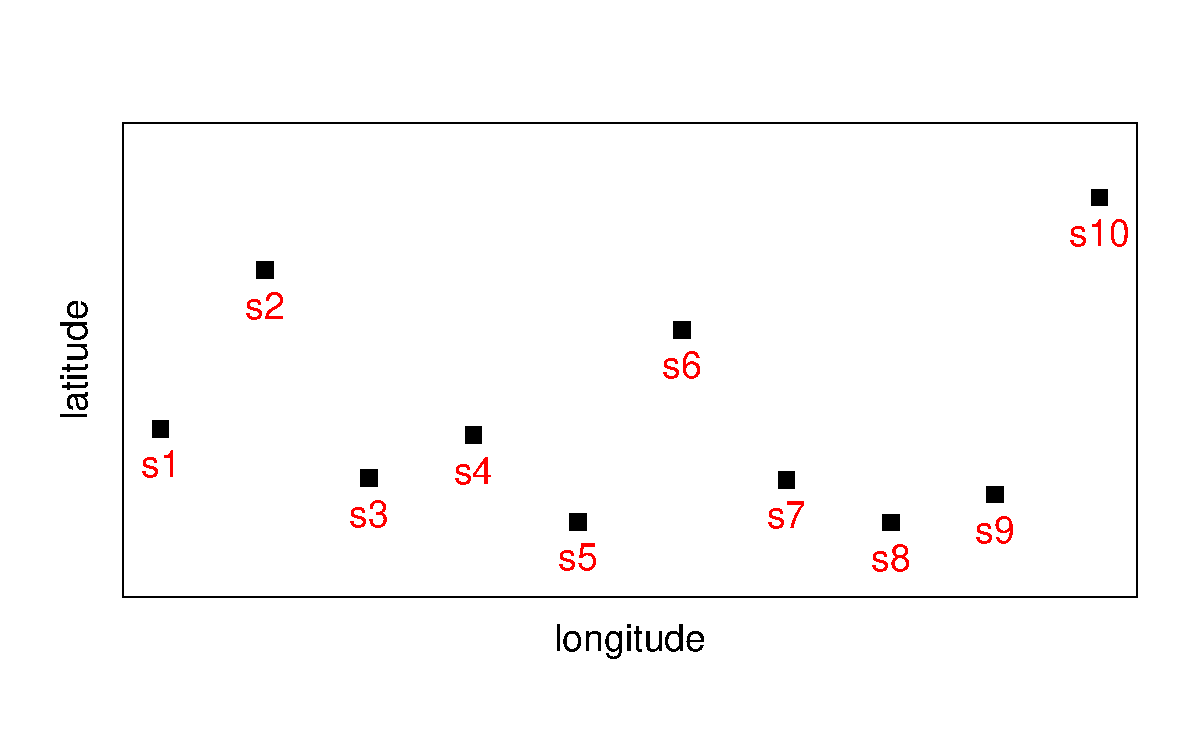
\includegraphics [width=0.8\textwidth, keepaspectratio]{graphs/location.pdf}
% \caption{Some arbitary saptial data at 10 random locations}
% \end{figure}


%\subsection{MSU data}

Since 1978 Microwave Sounding Units (MSU) measure radiation emitted by the earth's atmosphere from NOAA polar orbiting satellites. The different channels of the MSU measure different frequencies of radiation proportional to the temperature of broad vertical layers of the atmosphere. Tropospheric and lower stratospheric temperature data are collected by NOAA's TIROS-N polar-orbiting satellites and adjusted for time-dependent biases by the Global Hydrology and Climate Center at the University of Alabama in Huntsville (UAH)\footnote{\url{https://www.ncdc.noaa.gov/temp-and-precip/msu/overview}}. More information about how the data is been processed can be found in \cite{ChristySpencerBraswell2000}. Satellites do not measure temperature directly but measure radiances in various wavelength bands and then mathematically inverted to obtain the actual temperature. 

% Channel 2 mainly measures tropospheric temperatures, while Channel 4 measures temperatures in the lower stratosphere. The analysis of the satellite temperature record represented here begins in 1979.

\begin{figure}[H]
\label{MSU_data}
\centering
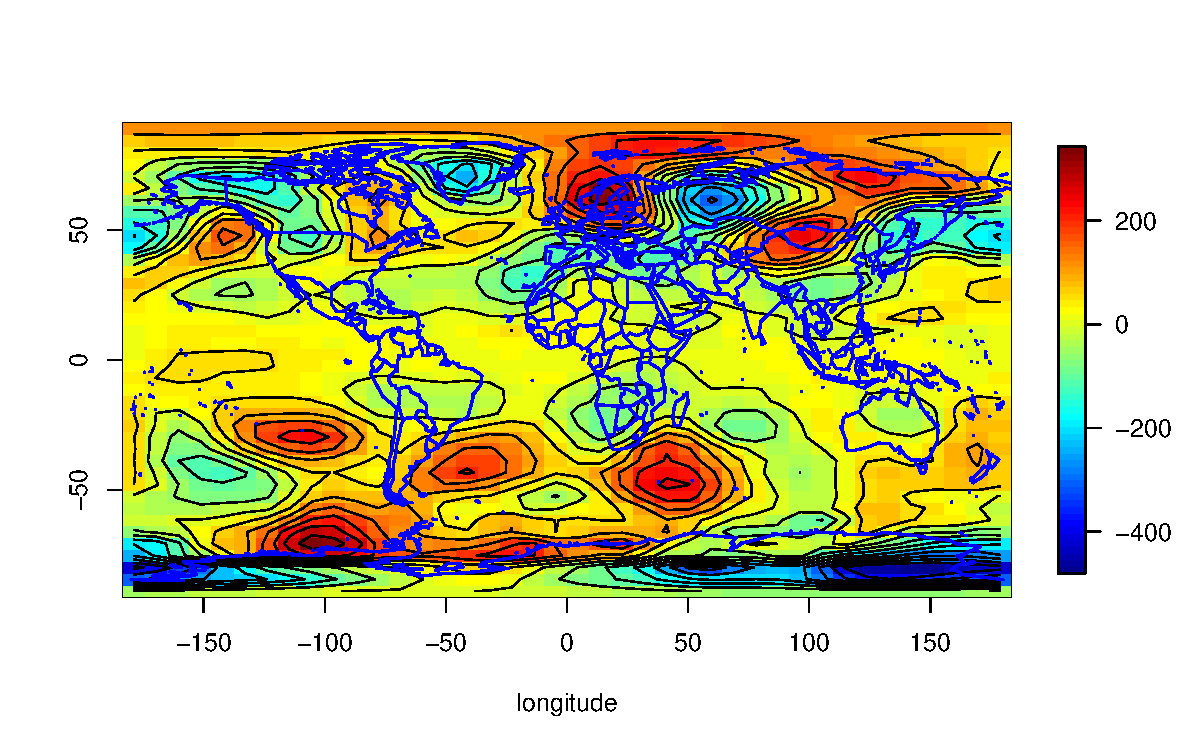
\includegraphics [width=0.8\textwidth, keepaspectratio]{graphs/MSU_data.pdf}
\caption{MSU data observed (without removing any spatial trends) in August 2002 : resolution $2.5^\circ \mbox{ latitude} \times 2.5^\circ \mbox{ longitude}$ (10368 gridded points).}
\end{figure}
\vfill
% The MSU data were observed at $2.5^\circ \mbox{latitude} \times 2.5^\circ \mbox{longitude}$ with total number of data observations of size 10368.


% \begin{figure}[H]
% \label{MSU_data_contour}
% \centering
% 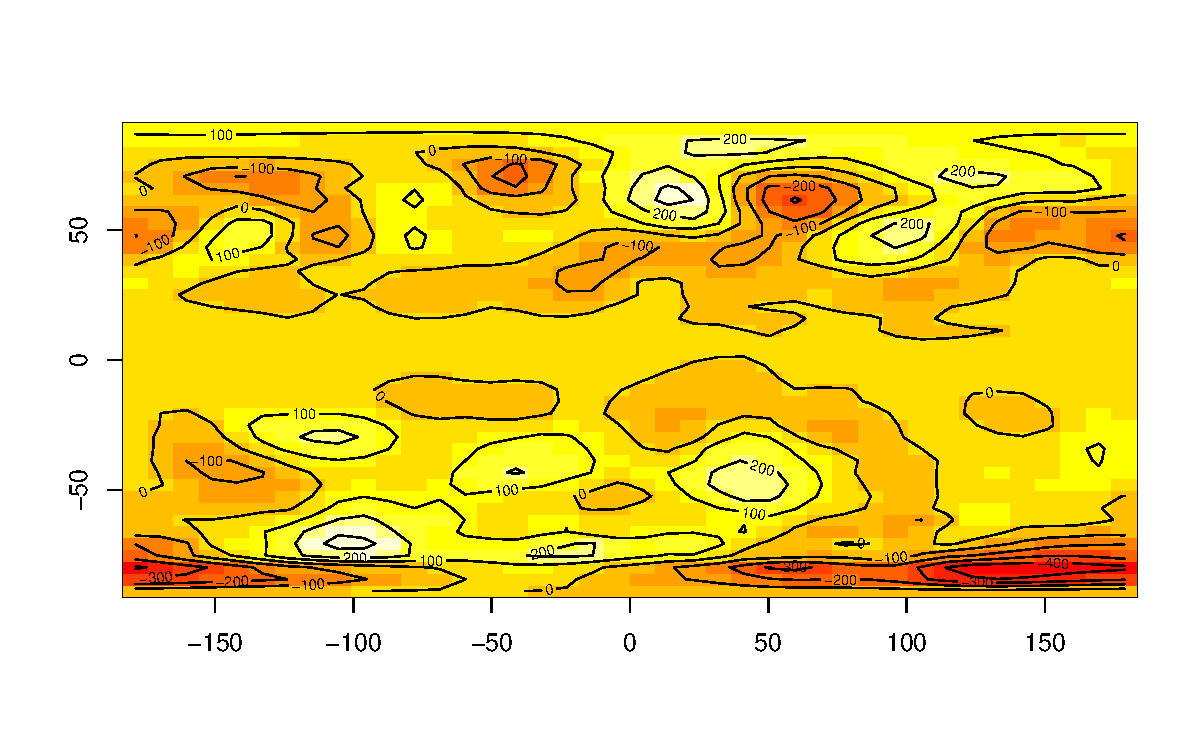
\includegraphics [height=4in, keepaspectratio]{MSU_data_contour.pdf}
% \caption{August 2002, MSU data contour plot : resolution $2.5^0 latitude \times 2.5^0 longitude$}
% \end{figure}

\begin{figure}[H]
	\begin{subfigure}{.5\textwidth}
		\centering
		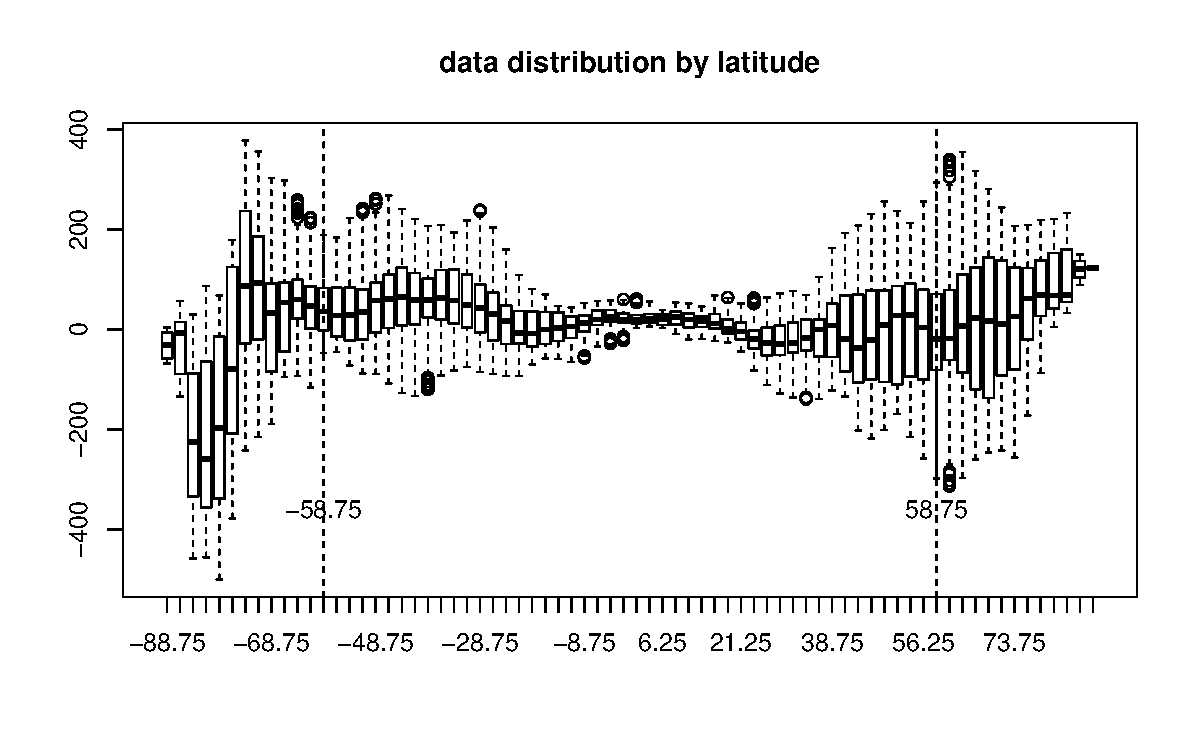
\includegraphics[width=1\linewidth]{graphs//MSU_data_latitude}
		\caption{distribution at each latitude}
		\label{MSU_data_latitude}
	\end{subfigure}
	\begin{subfigure}{.5\textwidth}
		\centering
		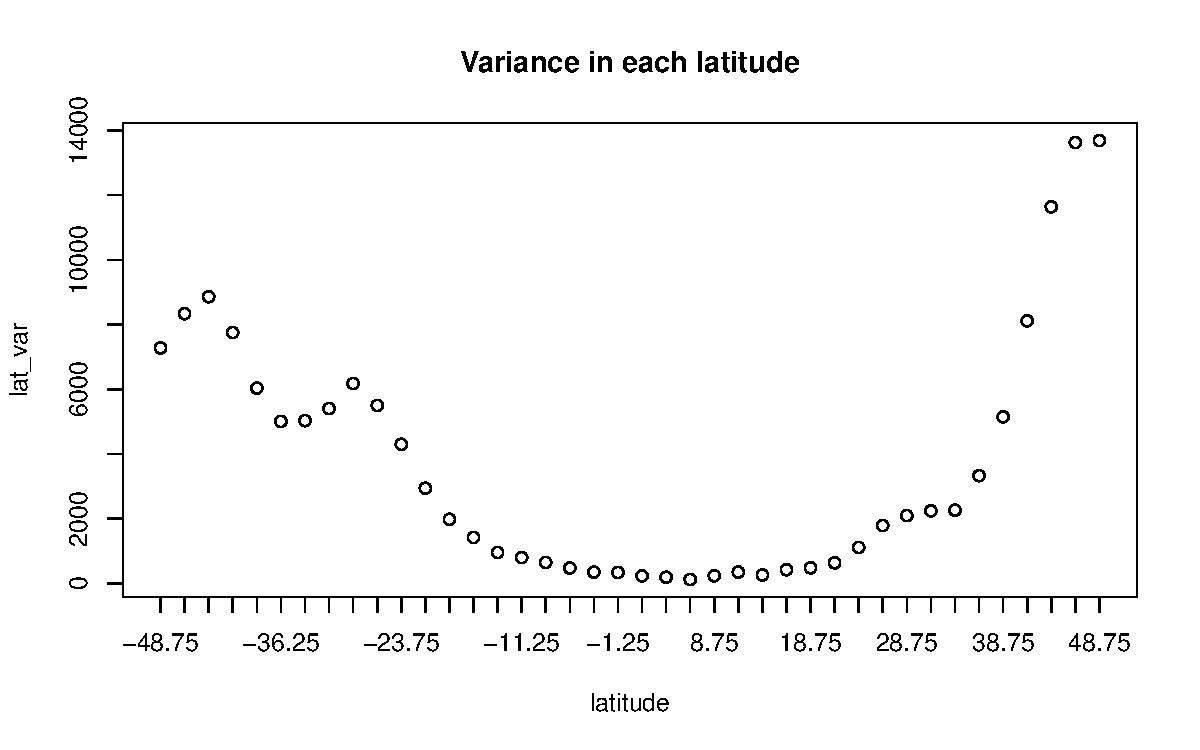
\includegraphics[width=1\linewidth]{graphs/MSU_data_var_lat}
		\caption{variance at each latitude}
		\label{MSU_data_var_lat}
	\end{subfigure}
	\caption[MSU data distribution at each latitude (data between $60^\circ S$ and $60^\circ N$ were considered)]{MSU data distribution at each latitude (data between $60^\circ S$ and $60^\circ N$ were considered)}
	\label{compare_varigram_sim_2}
\end{figure}


Level 3 Total Ozone Mapping Spectrometer (TOMS) data \footnote{\url{http://disc.sci.gsfc.nasa.gov/data/datapool/TOMS}} is another popluar global data set discussed literature which has more than 20000 sapatial points (gridded points) (\cite{Stein2007}, \cite{CressieJohannesson2008}, \cite{JunStein2008}). There were some missing values in this data set. \cite{Stein2007} used the average of 8 neighboring locations to replace the missing values. They used spherical harmonics with associated Legendre polynomials of up to 78 covariates to remove the spatial trends to study axially symmetry (discussed in chapter 4) of the global data. 

% Extracted from \cite{Stein2007} ``The Nimbus-7 satellite carried a Total Ozone Mapping Spectrometer (TOMS) instrument that measured total column ozone daily from November 1, 1978 to May 6, 1993. This satellite followed a Sun-synchronous polar orbit with an orbital frequency of 13.825 orbits a day (cycle time about 104 minutes). As the satellite orbited, a scanning mirror repeatedly scanned across a track about 3000 km wide, each track yielding 35 total column ozone measurements. This version of the data is known as Level 2 and is . "

\begin{figure}[H]
\label{TOMS_data}
\centering
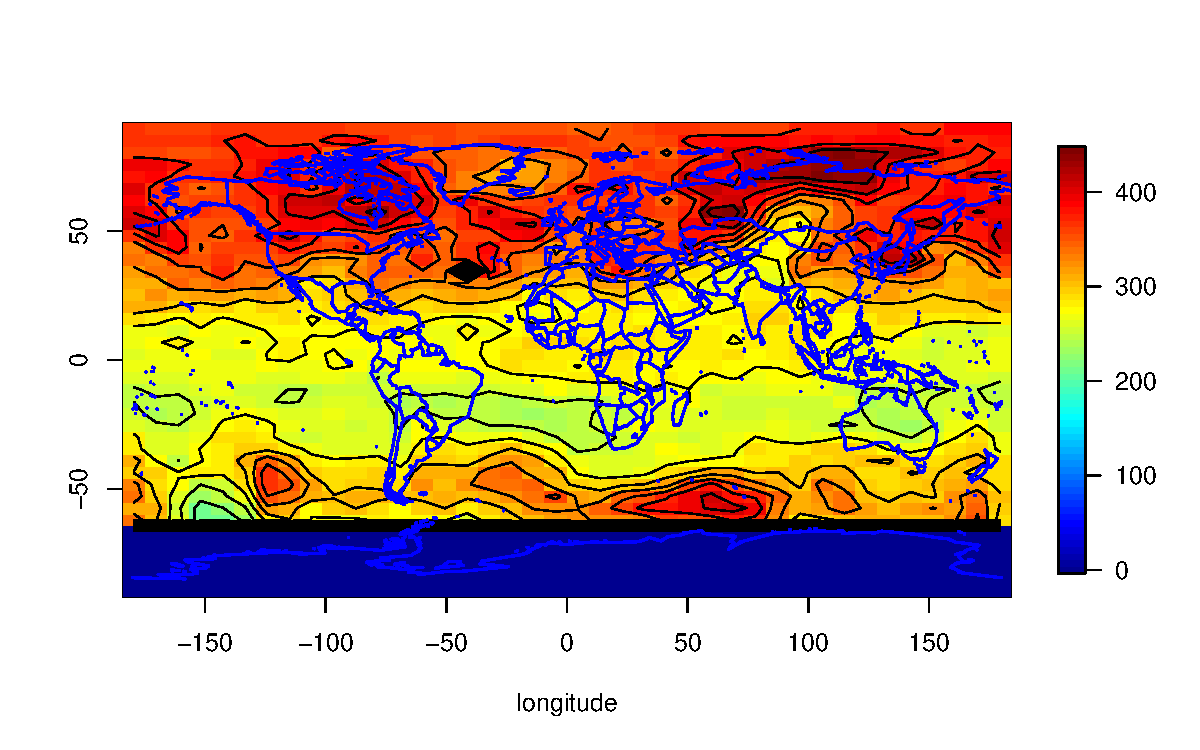
\includegraphics [width=0.8\textwidth, keepaspectratio]{graphs/TOMS_data.pdf}
\caption{TOMS data: resolution $1^\circ \mbox{latitude } \times 1.25^\circ \mbox{ longitude}$ in May, 1-6 1990. The instrument used backscattered sunlight, therefore measurements were not available south of $73^\circ S$ during this week.}
\end{figure}


\begin{figure}[H]
	\begin{subfigure}{.5\textwidth}
		\centering
		\includegraphics[width=1\linewidth]{graphs//TOMS_data_latitude}
		\caption{distribution at each latitude}
		\label{TOMS_data_latitude}
	\end{subfigure}
	\begin{subfigure}{.5\textwidth}
		\centering
		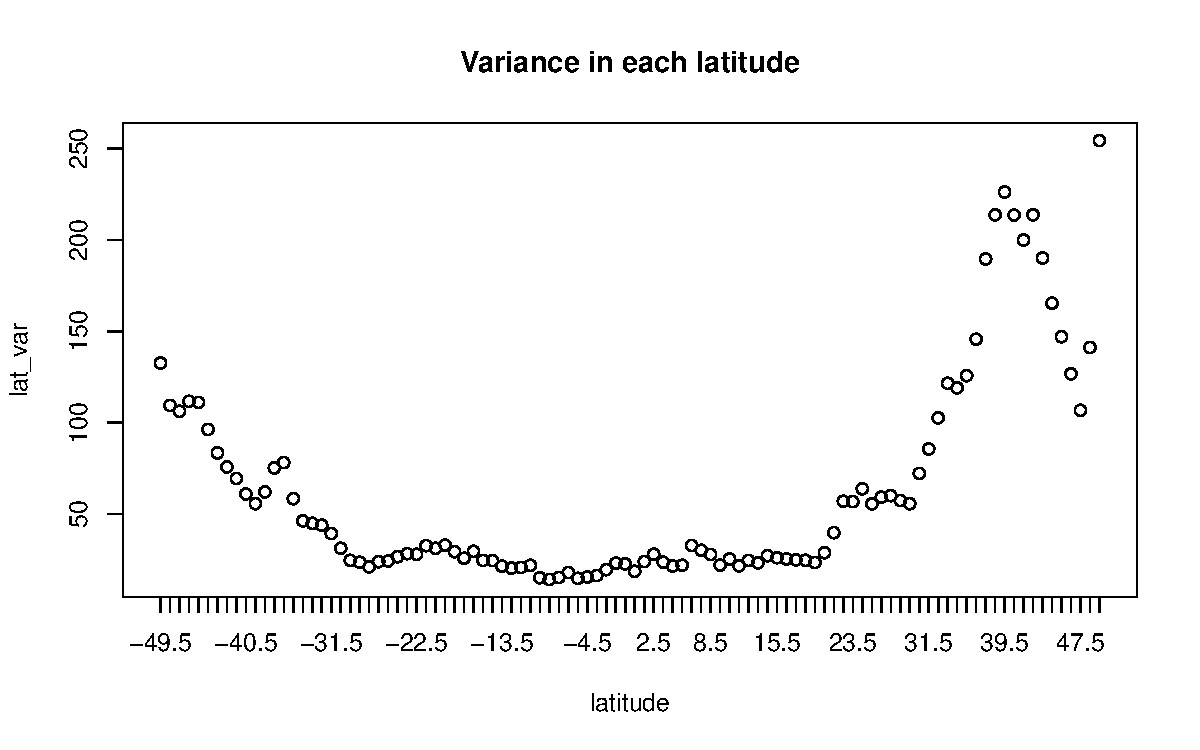
\includegraphics[width=1\linewidth]{graphs/TOMS_data_var_lat}
		\caption{variance at each latitude}
		\label{TOMS_data_var_lat}
	\end{subfigure}
	\caption[TOMS data distribution at each latitude (data between $50^\circ S$ and $50^\circ N$ were considered)]{TOMS data distribution at each latitude (data between $50^\circ S$ and $50^\circ N$ were considered)}
	\label{compare_varigram_sim_2}
\end{figure}


Both MSU and TOMS data demonstrate strong variation when it is closer to Earth's poles. This shows how complex is collecting Geo-spatial data, furthermore, it is very expensive and time consuming. Next we discuss about the challenges when modeling spatial data.  
\\

% \begin{figure}[H]
% \centering
% \includegraphics [width=0.8\textwidth, keepaspectratio]{graphs/TOMS_data_latitude.pdf}
% \caption{TOMS data: data distribution at each latitude (data between $50^\circ S$ and $50^\circ N$ were considered)}
% \label{TOMS_data_latitude}
% \end{figure}
% 
% \begin{figure}[H]
% \centering
% 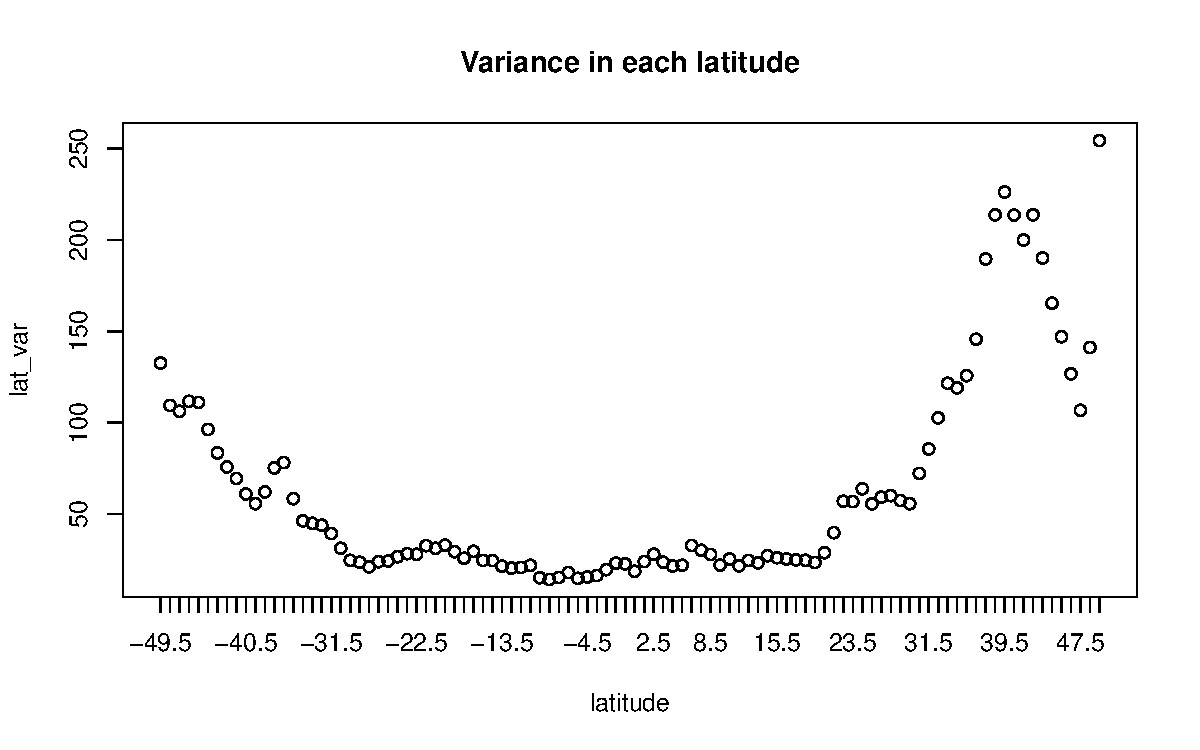
\includegraphics [width=0.8\textwidth, keepaspectratio]{graphs/TOMS_data_var_lat.pdf}
% \caption{TOMS data: between $50^\circ S$ and $50^\circ N$, the variance at each latitude (variance is almost zero near the equator)}
% \label{TOMS_data_var_lat}
% \end{figure}

% \subsection{Challenges}

\section{Literature}

There have been extensive statistical research on methodologies and techniques developed under the Euclidean space $R^d$. These approaches that are valid in $R^d$ have been applied to analyze global-scale data in recent years, due to global networks and satellite sensors that have been used to monitor a wide array of global-scale processes and variables. Some commonly used covariance models that are valid on $R^3$, 

\begin{table}[H]
\label{parameters}
\centering
\begin{tabular}{l|l|l}
\hline 
Family & C(h)  & Parameters \\ \hline \hline
$Mat\acute{e}rn$ &  $\frac{\sigma^2}{2^{\nu-1}\Gamma(\nu)} (\frac{h}{\phi})^{\nu} Y_{\nu}(\frac{h}{\phi})$  & $\nu, \sigma^2, \phi$  \\ 

Spherical & $\sigma^2(1-\frac{3h}{2\phi}+\frac{1}{2}(\frac{h}{\phi})^3)I_{0\le h\le \phi}$ & $\phi, \sigma^2$ \\

Exponential & $\sigma^2exp\{-(h/\phi)\}$ & $\phi, \sigma^2$  \\

Gaussian & $\sigma^2exp \{-(h/\phi)^2\}$ & $\phi, \sigma^2$  \\

Power* & $\sigma^2(C_0-(h/\phi)^{\alpha}$ & $\phi, \sigma^2$ \\ \hline
\end{tabular}
\caption{Commonly used covariance models in $\R^3$ * valid if $\alpha\in [0,2]$ }
\end{table}

However, this can have unforeseen impacts, such as making use of models that are valid in $R^d$ but in fact might not be valid under spherical coordinate systems. \cite{HuangZhangRobeson2011} have investigated some of commonly used covariance models that are valid in $R^d$, and they pointed out that many of those are actually invalid on the sphere. $Mat\acute{e}rn$ covariance models are widely used when modeling spatial data, but when the smoothness parameter ($\nu$) is greater than 0.5 it is not valid for the homogeneous processes on the Earth (\cite{Gneiting2013}). \\

Note that, as we will see later, the spectral representation of the process on the sphere is a summation of Legendre polynomials, which is distinct from its planar counterpart as represented by an integration of Bessel functions. This distinction can be understood through group representation theory, which is the basis for an exciting new line of research we are currently pursuing.\\



% \section{Literature}

		The main emplasis of this dissertation is on random process on a sphere and our primary focus is on covariance models on $S^2$. In general for covariance function defined on a sphere (\cite{Stein2007}) requires triple summation and required to estimate $\mathcal{O}(n^3)$ parameters. Geo-spatial (or satellite) data leads to large data sets and computational cost could be extremly expensive. In contrast, the covariance function  defined by \cite{Huang2012} requires to estimate $\mathcal{O}(n^2)$ parameters which is a huge reduction of computational complexity. All covariance models that are valid on $R^3$ are not valid on $S^2$ (\cite{HuangZhangRobeson2011}) and it is necessary to use $S^2$ instead of $R^3$ when studying about random processes on Earth and isotropy is often assumed (\cite{Yadrenko1983, Yaglom1987}). However, many studies have pointed out this assumption is not reasonable (\cite{Stein2007, JunStein2008, BolinLindgren2011}) for random processes on the sphere primarily on Earth. \cite{Stein2007} argued that Total Ozone Mapping Spectrometer (TOMS) data varies strongly with latitudes and homogeneous models are not suitable. Moreover, aerosol depth (AOD) from Multi-angle Imaging Spectrometer (MISR), Sea Surface Temperature (SST) from RRMM Microwave Imager (TMI) are some other example for anisotropy global data on a sphere (on Earth). \cite{JunStein2008} proposed flexible class of paramertric covariance models to capture the non stationarity.  In order to study non homogeneous processes on the sphere \cite{Jones1963} introduces the concept of axially symmetry, where the covarince between two spatial points depend on the longitudes only through their difference  between two points. This assumption is more plausible and reasonable when modeling spatial data. For example, temperature, moisture, etc. most likely symmetriy on longitudes rather than latitudes. \cite{Stein2007} used spherical harmonics to model axially symmetric process on a sphere. There are no practically useful parametric models available and to our knowledge only models available so far, \cite{stein1999} with 170 parameters to estimate and \cite{CressieJohannesson2008} more than 396 parameters to estimate. Monte Carlo Markov Chain (MCMC) is another approach to model non-stationary covariance models on a sphere. \cite{Lindgren2011} analyzed global temperature data with a non-stationary model defined on a sphere using Gaussian Markov Random Fields (GMRF) and Stochastic Partial Differential Equations (SPDE). Further \cite{BolinLindgren2011} constructed a class of stochastic field models using SPDEs and non stationary covariance models were obtained by spatially varying the parameters in the SPDEs, this method is more efficient than standard MCMC procedures. \cite{HitczenkoStein2012} applied first-order differential operators to an isotropic process to draw conclusions about the local properties of the processes. \cite{Li2013} used convolution methods with $Mat\acute{e}rn$-type kernal functions to capture the non-stationarity of random fields on a sphere. \cite{Huang2012} proposed a class of statistical processes that are axially symmetric and covariance functions that depend on longitudinal differences. Moreover, they proposed some ideas about longitudinally reversible processes and some motivations to construct axially symmetric processes on a sphere.


\section{The outline of this dissertation}
In Chapter 3 we explore some of the properties of commonly used covariance and variogram estimators on the circle based on Method of Moments (MOM). In contrasting to the results given in time series and the Euclidean space, the MOM covariance estimator is biased and the true \cov function is non idenentifiable based on the MOM estimator. On the other hand, the MOM variogram estimator is unbiased, but it can be shown to be inconsistent. Chapter 4 first introduce the random process on the sphere. We then discuss the homogeneous process and the spectral representation for its covariance function on the sphere. Our main focus on this chapter is the axially symmetric process and its covariance function representation through the discrete fourier transform. The parametric models for characterizing such processes are also discussed. In particular, we extend the models given in \cite{Huang2012} and provide some graphical properties of those models. These extended models will be fully implemented in Chapter 5 for axially symmetric data generation. In Chapter 5, we explore the result given in \cite{Huang2012} to implement an algorithm for axially symmetric data generation. In particular, we observe that our proposed method on data generation perform better based on cross variogram. Finally, Chapter 6 gives a summary of this research and provides some further research directions.   



% 
% 
% 
% Monte Carlo Markov Chain (MCMC) is another approach to model non-stationary covariance models on a sphere. \cite{BolinLindgren2011} (continuation of the work proposed in \cite{Lindgren2011} ) constructed a class of stochastic field models using Stochastic Partial Differential Equations (SPDEs). Non stationary covariance models were obtained by spatially varying the parameters in the SPDEs, they argue that this method is more efficient than standard MCMC procedures. 
% 
% \cite{HitczenkoStein2012} discuss about the properties of an existing class of models for axially symmetric Gaussian processes on the sphere. They applied first-order differential operators to an isotropic process. draw conclusions about the local properties of the processes. Under some restrictions they derived explicit forms for the spherical harmonic representation of these processes covariance functions, and make conclusions about the local properties of the processes.
% 
% $Mat\acute{e}rn$ covariance models are widely used when modeling spatial data, but when the smoothness parameter ($\nu$) is greater than 0.5 it is not valid for the homogeneous processes on the Earth surface with great circle distance. \cite{JeongJun2015} proposed $Mat\acute{e}rn$-like covariance functions for smooth processes on the earth surface that are valid with great circle distance (models were tested on sea levels pressure data).
% 
% \begin{enumerate}
% 
% \item Axially symmetry, which means that a process is invariant to rotations about the Earth's axis. The idea was first proposed by \cite{Jones1963}, where the covariance function depends on the longitudes only through their difference.
% 
% \item In the study of a random process on a sphere, homogeneity (covariance depends solely on distance between locations) was assumed. However, this assumption may not be reasonable for actual data. \cite{Stein2007} argued that Total Ozone Mapping Spectrometer (TOMS) data varies strongly with latitudes and homogeneous models are not suitable. Further, \cite{CressieJohannesson2008}, \cite{JunStein2008}, \cite{BolinLindgren2011} pointed out that homogeneity assumption is not reasonable.   
% 
% \item There are no methods to test axially symmetry in real data. However, this assumption is more plausible and reasonable when modeling spatial data. For example, temperature, moisture, etc. most likely symmetric on longitudes rather than latitudes. \cite{Stein2007} propose a method to model axially symmetric process on a sphere (the fitted model is not the best, but this was a good start).
% 
% \item There are no practically useful parametric models available, for our knowledge only models available so far, \cite{stein1999} with 170 parameters to estimate and \cite{CressieJohannesson2008} more than 396 parameters to estimate.
% %\blue{add description about the data}
% 
% \item When modeling spatial data stationary models are less useful;\cite{JunStein2008} has proposed flexible class of parametric covariance models to capture the non-stationarity of global data. They used Discrete Fourier Transform (DFT) to the data on regular grids and calculated the exact likelihood for large data sets. Furthermore, they used Legendre polynomials to remove the spatial trends when fitting models to global data.
% 
% \item \cite{Lindgren2011} analyzed global temperature data with a non-stationary model defined on a sphere using Gaussian Markov Random Fields (GMRF) and Stochastic Partial Differential Equations (SPDE)
% 
% \item Monte Carlo Markov Chain (MCMC) is another approach to model non-stationary covariance models on a sphere. \cite{BolinLindgren2011} (continuation of the work proposed in \cite{Lindgren2011} ) constructed a class of stochastic field models using Stochastic Partial Differential Equations (SPDEs). Non stationary covariance models were obtained by spatially varying the parameters in the SPDEs, they argue that this method is more efficient than standard MCMC procedures. There are many articles followed this techniques but we will not discuss more details about these methods.
% 
% \item Spatio-temporal mixed-effects model for dimension reduction was proposed by \cite{KatzfussCressie2011}. They used MOM parameter estimation method (similar approach in FRS). This work is also based on \cite{CressieJohannesson2008} spatial only Fixed Rank model. These methods are eventually focused on Bayesian approach and are less interested about topic.
% 
% \item The previous studies have argued that many processes on a sphere are not homogeneous, especially in latitude direction. \cite{Huang2012} proposed a class of statistical processes that are axially symmetric and covariance functions that depend on longitudinal differences. Moreover, they have proposed longitudinally reversible processes and some motivations to construct axially symmetric processes. The covariance models implemented in this dissertation are modified versions of the covariance models proposed by \cite{Huang2012}.  
% 
% \item \cite{HitczenkoStein2012} discuss about the properties of an existing class of models for axially symmetric Gaussian processes on the sphere. They applied first-order differential operators to an isotropic process. draw conclusions about the local properties of the processes. Under some restrictions they derived explicit forms for the spherical harmonic representation of these processes covariance functions, and make conclusions about the local properties of the processes.
% 
% %\item The issues associated when modeling axially symmetric spatial random fields on a sphere was discussed by \cite{Li2013}. They proposed convolution methods to generate random fields with a class of $Mat\acute{e}rn$-type kernel functions by allowing the parameters in the kernel function to vary with location. Moreover, they were able to generate flexible class of covariance functions and capture the non-stationary properties on a sphere. Used FFT to get the determinant and the inverse efficiently. Further, semi-parametric variogram estimation method using spectral representation was proposed for intrinsically stationary random fields on $S^2$.     
% 
% %\item \cite{HeatonKatzfussBerrettEtAl2014}
% 
% \item  $Mat\acute{e}rn$ covariance models are widely used when modeling spatial data, but when the smoothness parameter ($\nu$) is greater than 0.5 it is not valid for the homogeneous processes on the Earth surface with great circle distance. \cite{JeongJun2015} proposed $Mat\acute{e}rn$-like covariance functions for smooth processes on the earth surface that are valid with great circle distance (models were tested on sea levels pressure data).  
% 
% \end{enumerate}


%\blue{Fill the above table later  }

%\end{document} 


%%------------------------------------------------------------------%%
\chapter{Covariance and Variogram Estimation on the Cricle}
%%-------------------------process on a circle---------------------------------------%%
% \blue{
% 	discuss about data generation on a circle, 
% 	\begin{itemize}
% 		\item including circulant matrix
% 		\item why circulant matrix
% 		\item discuss covarince, biasness and the difficulties of estimation
% 		\item discuss variogram
% 		\item jones 1963
% 	\end{itemize}
% }

%%------------------------------------------------------------------%%
\section{Stationary process on a circle}
%%------------------------------------------------------------------%%

In this chapter we consider a real valued process $\{X(P): P\in S\}$ on the unit circle $S$, with finite second moment and continuity in quadratic mean. According to \cite{DUFOUR1976107} the process $\{X(P)\}$ can be represented in a Fourier series which is convergent in quadratic mean,

\beq \label{process_circle}
X(P) = A_0 + \sum_{n = 1}^\infty (A_n \cos(nP) + B_n \sin(nP).
\eeq


\begin{eqnarray}
	\nonumber
	\mbox{where} \quad A_0 &=&  \frac{1}{2\pi} \int_S X(P)dP, \\ \nonumber
	A_n &=& \frac{1}{\pi} \int_S \cos(nP)dP \\ 
	B_n &=& \frac{1}{\pi} \int_S \sin(nP)dP 
\end{eqnarray}

Let $P,Q$ be any two points on the circle, the covariance $R(P,Q)$ between the two points can be defined as,

\[
	R(P,Q) = E(X(P)X(Q)) = cov(X(P), X(Q))
\]

The process $X(P)$ is stationary if $E(X(P))$ is a constant and $R(P,Q)$ is function of the angular distance $\theta_{PQ}$ between $P$ and $Q$. If the process $X(P)$ is stationary on the circle,

\beq
cov(A_n, A_m) = a_n \delta(n,m) = cov(B_n, B_m), \quad \mbox{for $n, m \ge 0$}.
\eeq\\


Let $\{X(t_k)\}$ be a collection of gridded observations on a circle, with $t_k = (k-1)*2\pi/n, k = 1, 2, \cdots, n$. Let $C(\theta), \theta \in [0, \pi ]$ denote a stationary covariance function on the circle, the underlying process is stationary if it's covariance function solely depends on the distance $\theta$ and given as follows,

\beq
C(\theta) = cov(X(t_k+\theta), X(t_k)), \quad \quad \theta \in [0, \pi].
\eeq

The above covariance function can we can be written as a Fourier summmation (\cite{Roy1972})  

\beq
C(\theta) = \sum_{n=0}^\infty a_n \cos(n \theta),
\eeq

with $\sum_{n = 0}^\infty a_n < \infty$, and $a_n \ge 0$. Note that

\beq \nonumber
a_n  =\frac{2}{\pi}\int_0^\pi C(\theta) \cos(n\theta)d\theta \quad \mbox{and} \quad a_0  =\frac{1}{\pi}\int_0^\pi C(\theta)d\theta  .
\eeq 




%%------------------------------------------------------------------%%
\section{Estimation}
%%------------------------------------------------------------------%%

% The underlying process is stationary, if it's covariance function solely depends on the distance $\theta$,
% \beq
% C(\theta) = cov(X(t_k+\theta), X(t_k)), \quad \quad \theta \in [0, \pi].
% \eeq


Assuming the covariance function $C(\theta)$ on a cricle is a continuous function on $[0, \pi]$) and the gridded points $\{X(t_k)\}$ on a circle can be represented as $\utilde{X} = (X_1, X_2, \cdots, X_n)^T$. The variance-covariance matrix of the sample vector $\utilde{X} $ is given by $\Sigma$. Lets assume $E(X(t)) = \mu$ is unknown, and estimated by $\bar{X} = \frac{1}{n}\sum_{i=1}^{n} X(t_i)$.  Further, we can denote $\bar{X}$ in the following form,

\[
	\bar{X} = \frac{1}{n}{\bf 1}_n^T \utilde{X}
\]

\begin{eqnarray}
	\mbox{then,} \quad var(\bar{X}) &=& cov(\frac{1}{n}{\bf 1}_n^T \utilde{X}, \frac{1}{n}{\bf 1}_n^T \utilde{X}) \nonumber \\
	&=& \frac{1}{n^2}{\bf 1}_n^T \Sigma {\bf 1}_n \nonumber \\
	&=& \frac{1}{n} \left(C(0)+C(\pi)+2 \sum_{m=1}^{N-1}C(m 2\pi/n)\right) \nonumber
\end{eqnarray}


\begin{eqnarray*}
\mbox{When $n \to \infty$,}	\frac{1}{n} \left(2 \sum_{m=0}^{N}C(m 2\pi/n)\right) &=& \frac{1}{\pi} \frac{\pi}{N} \left( \sum_{m=0}^{N}C(m 2\pi/n)\right) \\ 
	&\to& \frac{1}{\pi} \int_0^\pi C(\theta)d\theta = a_0.
\end{eqnarray*}

\begin{eqnarray*}
	\mbox{Hence} \quad	var(\bar{X}) &=& \frac{1}{n} \left(2 \sum_{m=0}^{N}C(m 2\pi/n)\right) - \frac{1}{n}(C(0) + C(\pi)) \\
	&\to & a_0, \quad \quad \mbox{as $n \to \infty$}.
\end{eqnarray*}

 
\[
	\mbox{We can conclude that }	var(\bar{X}) \to \frac{1}{\pi} \int_0^\pi C(\theta)d\theta \quad \mbox{as $n \to \infty$}.  
\]


\begin{prop}

  Let $\bar{X}$ be an unbiased estimator for $\mu$ then $\bar{X}$ is not a consistent estimator for $\mu$, mean on a circle. \\
  
  {\bf proof:}
	If $\bar{X}$ is consistant we get the following, 
	\[
		P(|\bar{X} - \mu| > \varepsilon) \to 0.
	\]

	If $var(\bar{X}) \to 0$ and from Chebyshev's inequality we have

	\[
		P(|\bar{X} - \mu| > \varepsilon) \le \frac{var(\bar{X})}{\varepsilon^2} \to 0, \quad \mbox{for any $\varepsilon > 0$}.
	\]

	Therefore, $var(\bar{X}) \to 0$ is a sufficient condition for consistency, but it is not necessary. However, if we assume $\utilde{X}$ is multivariate normally distributed, then $\bar{X}$ follows normal distribution with mean $\mu$ and approximate variance $\sigma_0$. Then ($Z \sim N(0, 1)$)
	 
	 \begin{eqnarray*}
		P(|\bar{X} - \mu| > \varepsilon) &=& P\left(\frac{|\bar{X} - \mu|}{\sqrt{a_0}} > \frac{\varepsilon}{\sqrt{a_0}}\right) \\
		&=& P\left(|Z| > \frac{\varepsilon}{\sqrt{\sigma_0}}\right) \not\to 0  
	\end{eqnarray*}
	
	since $\frac{\varepsilon}{\sqrt{\sigma_0}}$ is a fixed constant for each fixed $\varepsilon > 0$.\\
	
\end{prop}

%-------------------------------------% 
\subsection{Estimation of covariance on a circle} \label{est_covariance}
%-------------------------------------%

We used method of moments (MOM) to estimate the covariance $C(\theta)$ on a circle, the estimator can be given by

\beq \label{covarince_estimator}
\hat{C}(\Delta \lambda) = \frac{1}{n}\sum_{i = 1}^n (X(t_i + \Delta \lambda) - \bar{X})(X(t_i) - \bar{X}), 
\eeq

where $\Delta \lambda = 0, 2\pi/n, 4\pi/n, \cdots, 2(N-1)\pi/n$.\\

We can show that the above estimator is a biased estimator for $C(\theta)$ .

\begin{eqnarray}
	\nonumber
	E(\hat{C}(\Delta \lambda)) &=& \frac{1}{n}\sum_{i = 1}^n E((X(t_i + \Delta \lambda) - \bar{X})(X(t_i) - \bar{X})) \\ \nonumber
	&=& \frac{1}{n}\sum_{i = 1}^n E((X(t_i + \Delta \lambda) - \mu - (\bar{X} - \mu))(X(t_i) -\mu - (\bar{X}) - \mu)) \\ \nonumber
	&=& \frac{1}{n}\sum_{i=1}^n cov(X(t_i+\Delta \lambda), X(t_i)) - \frac{1}{n}\sum_{i = 1}^n E((X(t_i + \Delta \lambda) - \mu)(\bar{X} - \mu)) \\ \nonumber
	& & -\frac{1}{n}\sum_{i = 1}^n E((X(t_i) - \mu)(\bar{X} - \mu)) + \frac{1}{n}\sum_{i = 1}^n E((\bar{X} - \mu)(\bar{X} - \mu)) \\ \nonumber
	&=& C(\Delta \lambda) -E((\bar{X} - \mu)(\bar{X} - \mu)) - E((\bar{X} - \mu)(\bar{X} - \mu)) \\ \nonumber 
	& & + E((\bar{X} - \mu)(\bar{X} - \mu)) \\ \nonumber
	&=& C(\Delta \lambda) - var(\bar{X}).
\end{eqnarray}

% Moreover,
% 
% \begin{eqnarray*}
% 	\nonumber
% 	var(\bar{X}) &=& E((\bar{X} - \mu)(\bar{X} - \mu)) = \frac{1}{n^2}\sum_{i = 1}^n \sum_{j=1}^n E(X(t_i) - \mu)(X(t_j) - \mu) \\ \nonumber
% 	&=&  \frac{1}{n^2}\sum_{i = 1}^n \sum_{j=1}^n cov(X(t_i), X(t_j)) = \frac{1}{n^2}\sum_{i = 1}^n \sum_{j=1}^n C(m*(i-j)*2\pi/n) \\ \nonumber
% 	&=& \frac{1}{n^2}\sum_{i = 1}^n \sum_{j=1}^n \left(a_0 + \sum_{k=1}^\infty a_k \cos(m*(i-j)*2\pi/n)\right) \\ \nonumber
% 	&=& a_0 + \sum_{k=1}^\infty a_k \left(\frac{1}{n^2}\sum_{i = 1}^n \sum_{j=1}^n \cos(m*(i-j)*2\pi/n)\right).
% \end{eqnarray*}
% 
% Now,
% 
% \begin{eqnarray*}
% 	& & \sum_{i = 1}^n \sum_{j=1}^n \cos(m*(i-j)*2\pi/n) \\
% 	&=& \sum_{i=1}^n \sum_{j=1}^n \left(\cos(m*i *2\pi/n)\cos(m*j*2\pi/n) + \sin(m*i *2\pi/n)\sin(m*j*2\pi/n) \right)\\
% 	&=& \left(\sum_{i=1}^n \cos(m*i *2\pi/n)\right)^2 + \left(\sum_{i=1}^n \sin(m*i *2\pi/n)\right)^2 = n^2
% \end{eqnarray*}
% 
% since for any integer $m$, we have
% 
% \[
% 	\sum_{k = 1}^{n} \cos(mk*2\pi/n) = \left\{\begin{array}{cc}
% 	0, & \mbox{for any integer $m \ne 0$,}  \\
% 	n, & \mbox{for $m = 0$}
% 	\end{array}
% 	\right. \mbox{ and }
% 	\sum_{k = 1}^{n} \sin(mk*2\pi/n) = 0.
% \]
% 
% Hence,
% \[
% 	var(\bar{X}) = a_0.
% \]
% 
% Therefore,
% \beq
% E(\hat{C}(\Delta \lambda)) = C(\Delta \lambda) - a_0.
% \eeq



% {\bf Note}: When $var(\bar{X}) \not\to 0$, we can not make the conclusion that $\bar{X}$ is not consistent. For consistency, we need to prove that


{\bf Remark 1} The MOM estimator $\hat{C}(\Delta \lambda)$ of the covariance function is actually a biased estimator with the shift amount of $a_0$. Therefore, if $a_0 = 0$ for a covariance function, we have the unbiased estimator $\hat{C}(\Delta \lambda)$. \\

{\bf Remark 2} If the gridded points were on a line, for example in time series, $E(\bar{X} - \mu)^2 \to 0$ as $n \to \infty$ under the assumption that the covariance function $C(\theta) \to 0$ when $\theta \to \infty$ (which is practically feasible), that is, $\bar{X}$ is consistent in the case of points on a line. In the case of circle, we might not have $C(\theta)$ close to 0 since $\theta$ is within a bounded region ($(0, \pi)$ for the circle) and we normally assume $C(\theta)$ is continuous for $\theta$. \\


%-------------------------------------%
\subsection{Estimation of variogram on a circle}
%-------------------------------------%

The theoretical variogram function is given by,
\beq
\gamma(\theta) = C(0) - C(\theta).
\eeq
and the MOM estimator for the variogram is given by,

\beq
\hat{\gamma}(\Delta \lambda) = \frac{1}{2n} \sum_{i=1}^n (X(t_i + \Delta \lambda) - X(t_i))^2.
\eeq

We can show that variogram estimator through MOM is an unbiased estimator, 

\begin{eqnarray*}
	E(\hat{\gamma}(\Delta \lambda)) &=& \frac{1}{2n} \sum_{i = 1}^n E(X(t_i + \Delta \lambda) - X(t_i))^2 \\
	&=& \frac{1}{2n} \sum_{i = 1}^n E((X(t_i + \Delta \lambda)-\mu) - (X(t_i) - \mu))^2 \\
	&=& \frac{1}{2n} \sum_{i = 1}^n cov(X(t_i + \Delta \lambda) - X(t_i), X(t_i + \Delta \lambda) - X(t_i)) \\
	&=& \frac{1}{2n} \sum_{i = 1}^n \left\{ cov(X(t_i + \Delta \lambda), X(t_i + \Delta \lambda)) + cov(X(t_i), X(t_i)) \right. \\
	& & \left. - 2cov(X(t_i + \Delta \lambda), X(t_i)) \right\}\\
	&=& \frac{1}{2n} \sum_{i = 1}^n \left( C(0) + C(0) - 2C(\Delta \lambda)\right) \\
	&=& C(0) - C(\Delta \lambda) = \gamma(\Delta \lambda).
\end{eqnarray*}
 
\blue{need to prove consistency}


%-------------------------------------%
\section{Data generation on a circle}
%-------------------------------------% 



First, we will discuss how to generate correlated data at $n$ girdded points on a circle when the covarince function is defined and compare above covariance and variogram estimators. Since the observed data are correlated, the covariance function can be written as a function of distance (angle). For the data generation process we will use exponential family and power family covariance function as given below, 

\beq \label{exp_cov} 
C(\theta) = C_1e^{-a|\theta|} \quad a>0, C_1>0
\eeq

\beq \label{power_cov} 
C(\theta) = c_0 - (|\theta|/a)^{\alpha} \quad a>0, \alpha \in (0,2] \mbox{ and } c_0 \ge \int_0^\pi
			(\theta/a)^{\alpha} \sin \theta d \theta
\eeq


where $\theta = i*\Delta\lambda = \pm i*2\pi/n, i=1,2,\cdots,\floor{n/2}$ \\

\begin{figure}
	\centering
	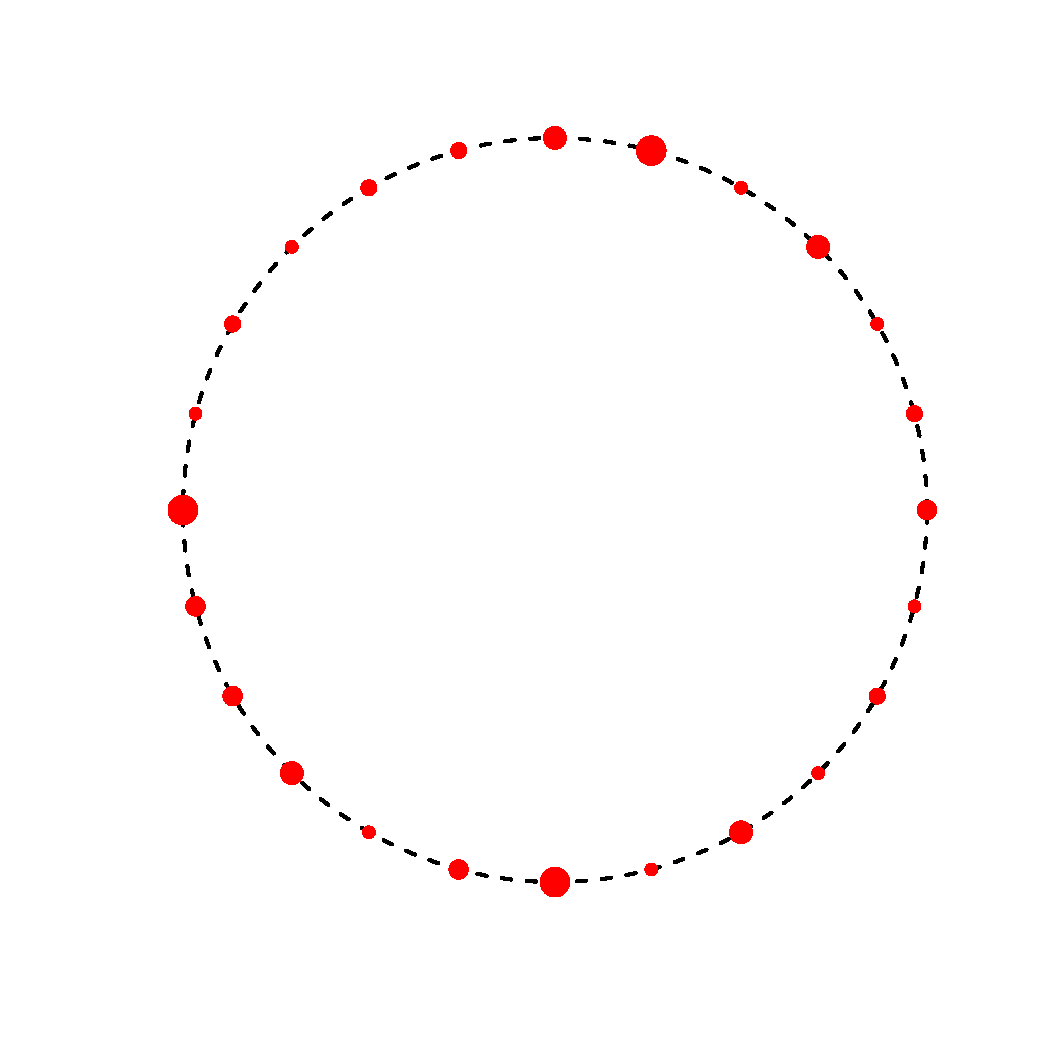
\includegraphics[width=0.5\textwidth]{graphs/process_circle}
	\caption {Random process on a circle at 24 points ($\Delta\lambda = 15^0$), the red dots represent the  observed values at a given time and each point is associated with a random process of it's own.}
\end{figure}

Clearly, each location is correlated with other $n-1$ locations and $C(\theta) = C(-\theta)$ the variance-covariance matrix $\Sigma$ is circulant and will be in the following form,   


\begin{eqnarray*}
	\Sigma &=& circ(C(0),C(\delta), C(2\delta), \cdots, C((N-1)\delta), C(\pi),  C((N-1)\delta), \cdots, C(\delta)) \\
	&=& \left(\begin{array}{ccccccc}
	C(0)      & \cdots & C((N-1)\delta ) & C(\pi) &  C((N-1)\delta ) & \cdots & C(\delta) \\
	C(\delta) & \cdots & C((N-2)\delta) & C((N-1)\delta) &  C(\pi)  & \cdots & C(2\delta) \\
	C(2\delta) & \cdots & C((N-3)\delta) & C((N-2)\delta) &  C((N-1)\delta) & \cdots & C(3\delta)\\
	\vdots    & \vdots  & \vdots  & \vdots  & \vdots  & \vdots  & \vdots  \\
	C(\delta) & \cdots & C(\pi) &  C((N-1)\delta) & C((N-2)\delta)  & \cdots & C(0) 
	\end{array} \right) \\
	&=& Q\Lambda Q^T,
\end{eqnarray*}

where $\delta = 2\pi/n,\ \Lambda=\{\lambda_1, \lambda_2,\cdots,\lambda_n\}$ and $Q=\{\psi_1, \psi_2,\cdots,\psi_n\}$ are the respective eigen values and eigen vectors of the above circulant matrix. Now using singular value decomposition (SVD) we can obtain the correlated data $\utilde{X}$ on a circle as follows,

\[
	\utilde{X} = \Sigma^{1/2}*Z = Q\Lambda^{1/2}Q^T*Z 
\]

where $Z\sim N(\utilde{0},1_{n})$.

%-------------------------------------%
\subsection{Compare covariance estimator} 
%-------------------------------------%

% \beq\label{cov:circle1}
% C(\theta) = \frac{1}{n_L} \sum_{i=1}^{n_L} (X(a_i+\theta)\cdot X(a_i))-(\overline{X(a)})^2
% \eeq

	      In section \ref{est_covariance} we proved that, in general the covarince estimator (\ref{covarince_estimator}) on a circle is biased, with a bias of $var(\bar{X})$. In order to make things simple we set $C_1, a = 1$ when $\alpha = 0.5$ $c_0 \ge \int_0^\pi(\theta)^{0.5} \sin \theta d \theta$, from Fresnel intergal it can be shown that $c_0 \ge 2.4353$. Now we compare the covariance estimator to it's theoretical covarince given by equations \ref{exp_cov} and \ref{power_cov}. We computed the MOM estimator $\hat{C}(\theta)$ with 48 gridded observations on the circle from 500 simulations.
	      	      
	      \begin{figure}[H]
	      	\label{covarince_circle}
	      	\centering
	       	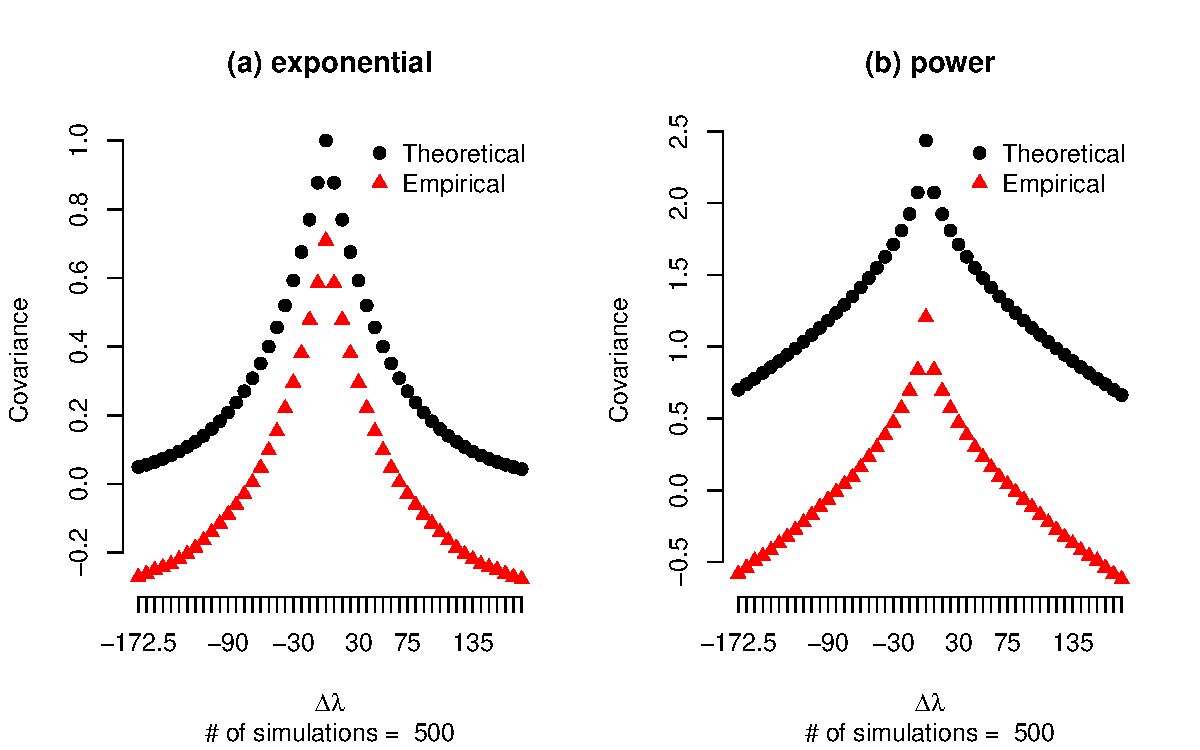
\includegraphics[width=0.9\textwidth]{graphs/covarince_circle}
	      	\caption {Theoretical and empirical covariance (with bias) comparison on a circle}
	      \end{figure}

	      {\bf Remark 1:} We noticed that the shift between theoretical and empirical values were approximately equal to $a_0$ and we can obtain $a_0$ for the above covarince as follows,
	      \[
	    \mbox{exponential : }  	a_0 = \frac{C_1}{a\pi}(1 - e^{-a\pi})
	      \]

	      \[
	    \mbox{power : }  	a_0 = c_0 - \left(\frac{\pi}{a}\right)^{\alpha}\frac{1}{\alpha + 1}
	      \]

	      Now we consider the following covariance function, after subtracting $a_0$ from $C(\theta)$.
	      \[
	      	D(\theta) = C(\theta) - a_0.
	      \]
      
        If the new covariance function $D(\theta)$ was used to generate the data on a circle then the theoretical and empirical values will match perfectly.
        
	      % \beq \label{cov:circle1}  
	      % C(\theta) = \frac{1}{n_L} \sum_{i=1}^{n_L} (X(a_i+\theta) \cdot X(a_i)) 
	      % \eeq
	      	      
	      \begin{figure}[H]
	      	\centering
	      	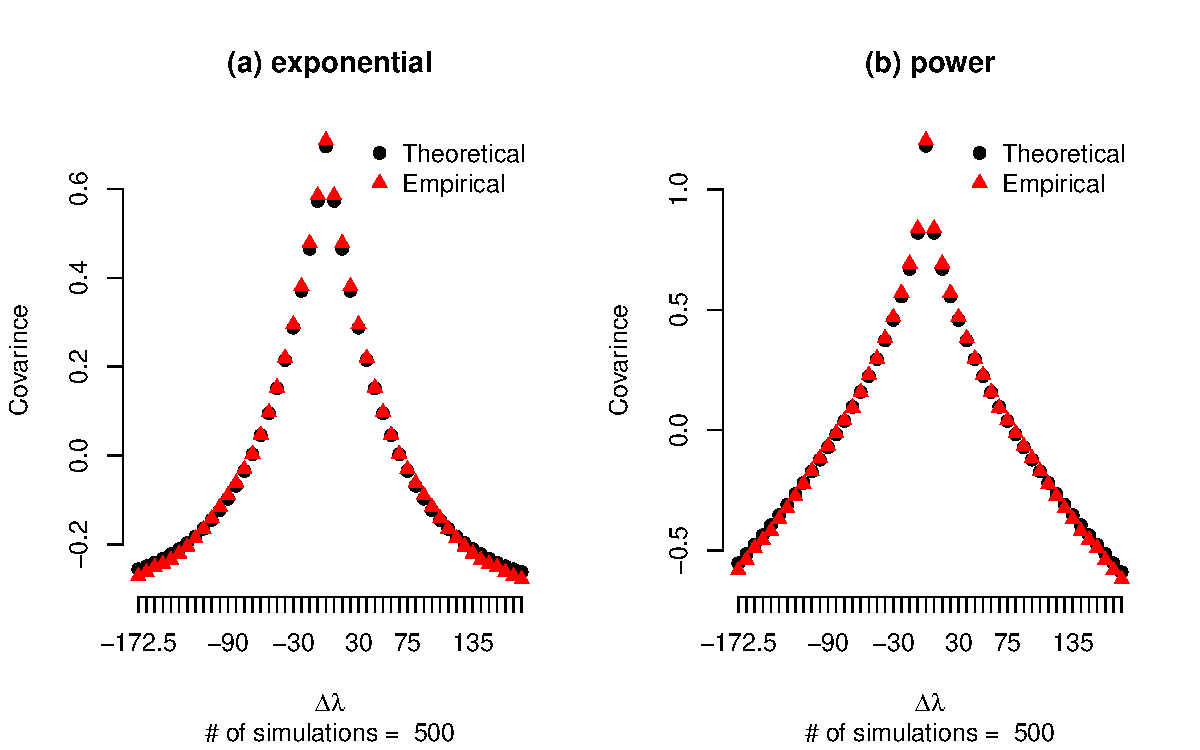
\includegraphics[width=0.9\textwidth]{graphs/covarince_circle_remove_a0}
	      	%graph from data genaration summary doc line 194 
	      	\caption {Theoretical and empirical covariance comparison on a circle}
	      \end{figure}
	      	      
{\bf Remark 2:} If the process is a zero mean process the covariance estimator will be unbiased ($i.e. Var(\bar{X}) = 0$) hence we will get a perfect match between theoretical and empirical values.\\

{\bf Remark 3:} We have shown that covariance estiamtor is biased and the biasness will approach to $a_0$. When covariance function is unknown the biaseness $a_0$ is also known and the biasness cannnot to estimated (cannot find the variance of $\bar{X}$) from one circle, however in both exponential and power covariance models it can be estimated if multiple copies of data (on a circle) were generated {\em i.e.} $\hat{a} = var(\bar{X})$. 

	      \begin{figure}[H]
	      	\centering
	      	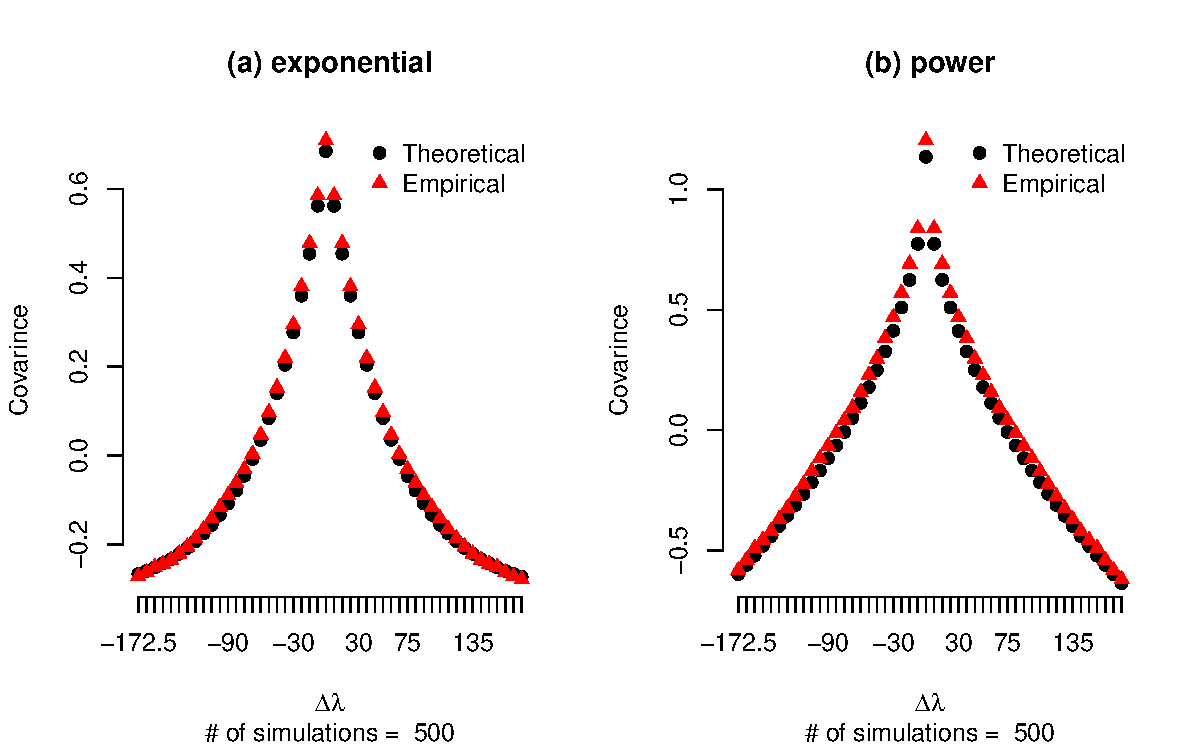
\includegraphics[width=0.9\textwidth]{graphs/covarince_circle_estimate_a0}
	      	%graph from data genaration summary doc line 194 
	      	\caption {Theoretical and empirical covariance comparison on a circle, after removing biasness}
	      \end{figure}
	      

	      	      
%-------------------------------------%
\subsection{Compare variogram estimator} 
%-------------------------------------%

We proved that in general the variogram estimator is unbiased \blue{and consistent}. Since the semi variogram $\gamma(\theta) = C(0) - C(\theta)$,  the theoretical variogram based on exponential and power covariance functions can be given in the following form,   

\[
	\mbox{exponential : }\gamma(\theta) = C(0) - C(\theta) = C_1(1-e^{-a|\theta|})
\]

\[
	\mbox{power : } \gamma(\theta) = C(0) - C(\theta) = C_1(1-e^{-a|\theta|})
\]

We computed the variogram estimator $\hat{\gamma}(\theta)$ with 48 gridded observations on the circle from 500 simulations and there is a better fit between theoretical and empirical values compared to covariance models.


\begin{figure}[H]
	\centering
	%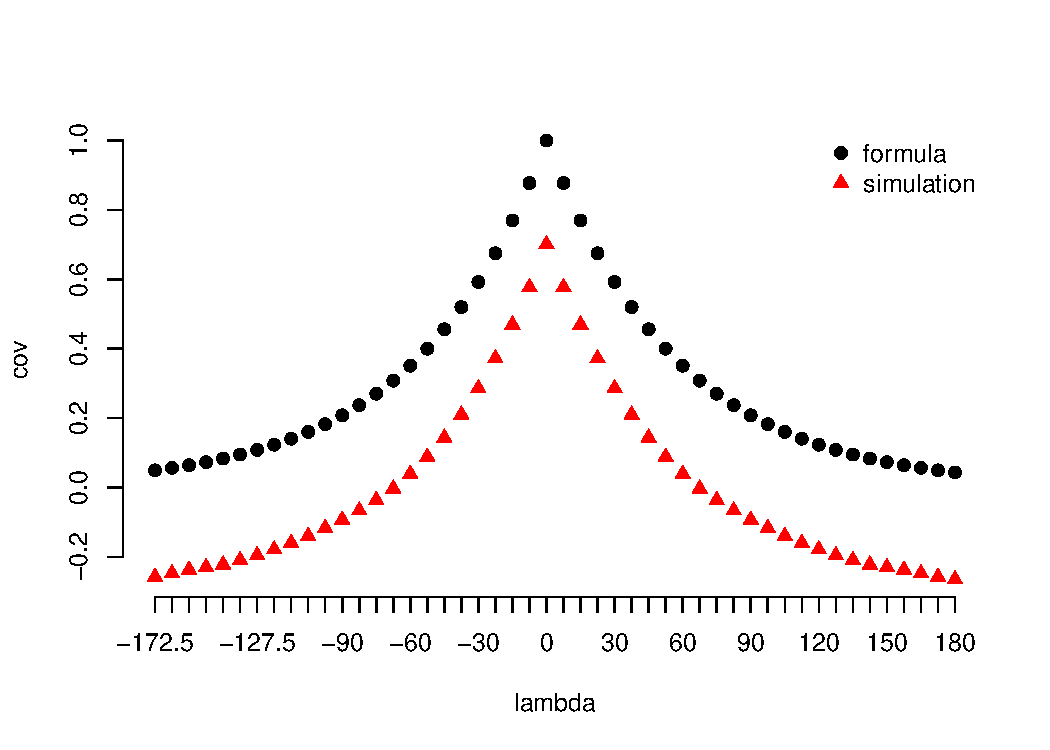
\includegraphics[width=0.65\textwidth]{graphs/Summary-covarince_circle_1}
	%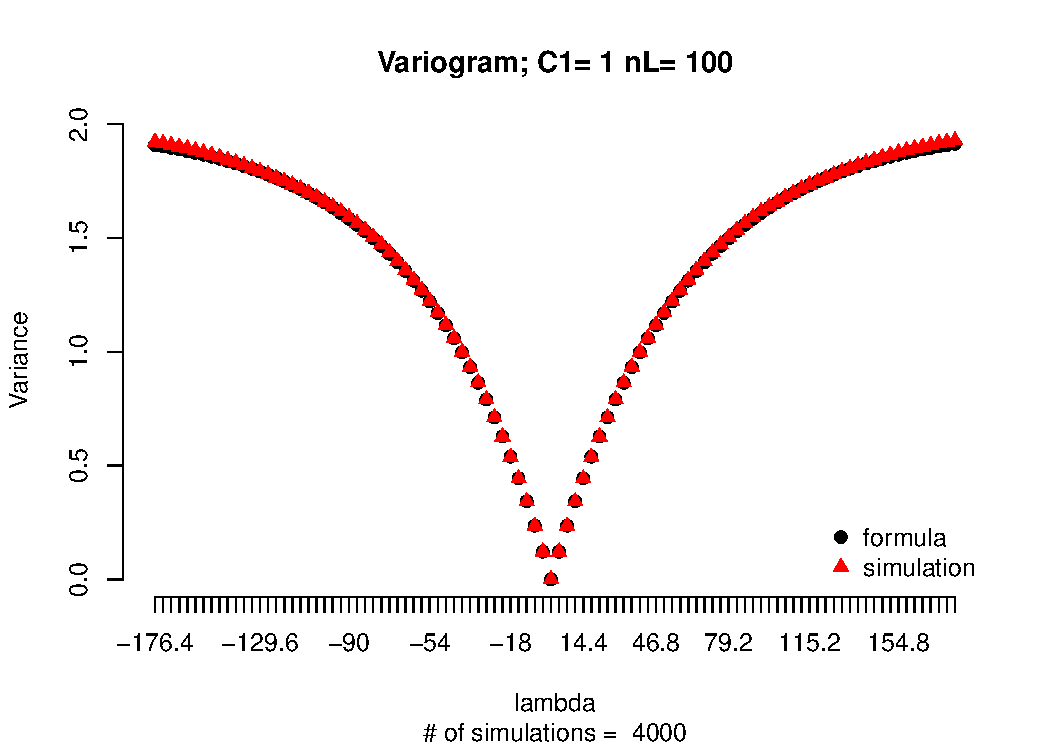
\includegraphics[width=0.65\textwidth]{graphs/variogram_plot_4000}
	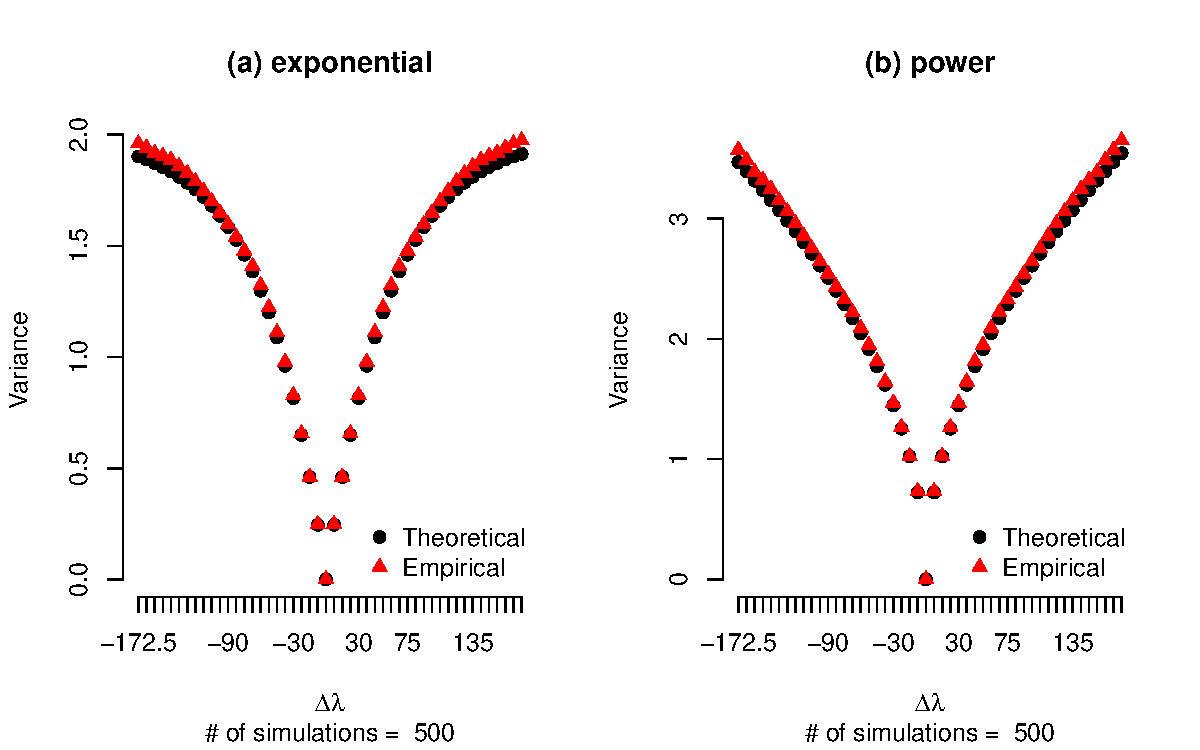
\includegraphics[width=0.9\textwidth]{graphs/variogram_plot_500}
	%graph from data genaration summary doc line 177 
	\caption {Theoretical and empirical comparison for variogram on a circle}
\end{figure}

{\bf Remark 4} \blue{should we talk about how $n_L$ is related with number of simulations }



%%------------------------------------------------------------------%%
\chapter{Random Process on a Sphere (due August 21)}
%%-------------------------Random process on sphere---------------------------------------%%


Suppose $X \in \{X(s): s\in D\}$, defined in a common probability space $s \in S^2$: $X(s)$ is a random process or a spatial processes on the sphere $S^2$ with radius $r$ and $s$ represents any location on sphere by latitude $L$ and longitude $l$, where $0 \ge L \ge \pi$ and $-\pi \ge l \ge \pi$.\\


%%------------------------------------------------------------------%%
\section{Covariance on sphere} 
%%------------------------------------------------------------------%%

The random process $X(\cdot)$ is said to be homogeneous (or isotropy) on $S^2$ if second moment is finite and invariant under the rotations on the sphere with constant mean. Similarly, we can define an isoropic random process on a sphere as, 

\begin{eqnarray*}
	E(X(s) &=& \mu \quad \mbox{for any } s\in S^2 \\
	Cov(X(s_1),X(s_2)) &=& C(\theta_{s_1s_2}) 
\end{eqnarray*}

where $\theta_{s_1s_2}$ is the spherical angle between two locations $s_1,s_2$. For a unit sphere, the distance between the two locations can be defined as great circle distance ($\gcd_{s_1s_2}$) or chordal distance ($ch_{s_1s_2}$) as follows,

\begin{eqnarray*}
	\theta_{s_1s_2}  &=& \arccos\left(\sin(L_1)\sin(L_2) + \cos(L_1)\cos(L_2)\cos(l_1-l_2)\right)\\
	% gcd_{s_1s_2}    &=&  1\cdot\theta_{s_1s_2}\\
	% ch_{s_1s_2}     &=& 2\sin (\theta_{s_1s_2}/2)
\end{eqnarray*}

In the case of $\R^d$, non-negative definite is a necessary and sufficient condition for a valid covariance function defined on $\R^d$ (\ref{cov_pd}). Similarly, a real continuous function $C(\cdot)$ defined on the sphere is a valid covariance function if and only if it is non-negative definite,

\beq
\sum_{i,j=1}^{N} a_i a_j C(\theta_{s_1s_2}) \ge 0,
\eeq
for any integer $N$, any constants $a_1, a_2, \ldots, a_N$, and any locations $s_1, s_2, \ldots, s_N \in S^2$.

Let $P_{k}^{\nu}(\cos\theta)$ be the ultraspherical polynomials defined by the following infinite summation,

\beq
  \frac{1}{(1 - 2c\cos\theta + c^2)^{\nu}} = \sum_{k=0}^{\infty}c^{k} P_{k}^{\nu}(\cos\theta) \quad \nu>0
\eeq


\[
\mbox{When $\nu = 0$, } P_{k}^{0}(\cos\theta) = \cos (k\theta)
\]

Accoriding to \cite{schoenberg1942}, a real continous function $C(\theta)$ is a valid covariance function on $S^d$, where $d=1,2,\ldots$, if and only if it can be written in the following form

\beq
C(\theta) = \sum_{k = 0}^\infty c_kP_k^{(\nu)}(\cos\theta), \quad \nu=\frac{1}{2}(d-1)
\eeq

where $\forall c_k\ge 0$ and $\sum c_k < \infty$. \\

Suppose $C(\cdot)$ is a covariance functions that is valid in $S^d$ then it is valid on $S^m$ where $d\le m$. In general we have the following property,

\[
S^1 \subset S^2 \subset \cdots S^{d} \subset \cdots S^{\infty}
\]


\[
C(S^1) \supset C(S^2) \supset \cdots C(S^d) \supset \cdots C(S^{\infty})
\]

and covariance functions that are valid on $S^m$ may not be valid on $S^d$ where $m>d$ \blue{example?}.\\

In chapter 3 we discussed about random processes on a circle and the covariance on a circle ($d=1$) was expressed as follows,

\beq
C(\theta) = \sum_{k = 0}^\infty c_k\cos (k\theta)
\eeq

Since $\cos\theta \in S^1$ clearly $\cos\theta \in S^2$ and from the properties of covariance discussed in chapter 1, $P_k\cos\theta \in S^2$ where $P_k$ is a Legender ploynomial. Therefore, when $d=2$ the covarince on a sphere ($S^2$) can be expressed as follows,

\beq \label{covs2_sum}
C(\theta) = \sum_{k = 0}^\infty c_kP_k(\cos\theta)
\eeq

% \blue{?if a covariance function is not valid on $S^r$ it is not valid on $S^d \quad d > r$ (example).}\\

Since the Legendre polynomials are orthogonal we have

\[
	\int_{-1}^{1} P_{n}(x)P_{m}(x)dx = \frac{2}{2n+1}\delta_{nm}
\]

and on a sphere the coefficients $c_k$ can be obtained by

\beq \label{covs2_coef}
c_{\nu} = \frac{2\nu+1}{2}\int_0^{\pi} C(\theta)P_{\nu}(\cos\theta)d\theta. \quad \nu = 0,1,2,\ldots
\eeq

One can directly use the above integral to evalute the validity of a covariance function on the sphere by checking if $c_k$ is non-negative and $\sum c_k < \infty$ .\\ 

All covariance models that are valid on $\R^d$ are not valid on the sphere ($S^2$), \cite{HuangZhangRobeson2011} evaluated the validity of commonly used covariance on a sphere that are valid on $\R^d$, they showed that some models are not valid on the sphere and some models are valid only for certain parameter values.  
 

\begin{table}[H]
	\label{valid_cov_models}
	\centering
	\begin{tabular}[htb]{lll} \hline \hline
		Model & Covariance function & Validity  $S^2$           \\   \hline Spherical  &
		$\left(1-\frac{3\theta}{2a} + \frac{1}{2}
		\frac{\theta^3}{a^3}\right){\bf 1}_{(\theta \le a)}$ & Yes   \\
		[2ex]
		Stable     & $\exp\left\{-\left(\frac{\theta}{a}\right)^\alpha\right\}$ & Yes for $\alpha \in (0,1]$  \\
		      &                     & No for $\alpha \in (1,2]$ \\ [2ex] \hspace{0.2in} Exponential &
		$\exp \{-\left(\frac{\theta}{a}\right) \}$ & Yes \\ [2ex]
		\hspace{0.2in} Gaussian & $\exp\left\{-\left(\frac{\theta}{a} \right)^2
		\right\}$  & No \\ [2ex]
		Power$^*$   & $c_0 - (\theta/a)^\alpha$ & Yes for  $\alpha \in (0,1] $  \\
		& & No for $\alpha \in (1,2]$ \\ [2ex]
		Radon transform of order 2         & $e^{-\theta/a}(1+\theta/a)$ &
		No        \\ [2ex] Radon transform of order 4         &
		$e^{-\theta/a} (1+\theta/a+\theta^2/3a^2)$  & No  \\ [2ex] Cauchy &
		$(1+\theta^2/a^2)^{-1}$ &  No      \\ [2ex] Hole - effect & $\sin
		a\theta / \theta$ & No    \\ \hline \hline
	\end{tabular}
	\caption{Validity of covariance functions on the sphere, $a >
		0,\theta \in [0,\pi]$. $^*$When $\alpha \in (0,1]$, power model is
			valid on the sphere  for some $c_0 \ge \int_0^\pi
			(\theta/a)^{\alpha} \sin \theta d \theta$.} \label{tab:t1}
				
	\end{table}
	
	Furthermore, \cite{Gneiting2013} argued that Mat$\acute{e}$rn covariance function is valid on the sphere when the smoothness parameter $\nu\in(0,1/2)$ and it is not valid if $\nu>1/2$. \cite{Yadrenko1983} showed that if $K(\cdot)$ is valid isotropic covariance function on $\R^3$ then
	
	\[
		C(\theta) = K(2\sin(\theta/2))
	\]
	
	is a valid isotropic covariance function on the unit sphere (where $\theta$ is $gcd$).
	
	%%------------------------------------------------------------------%%
	\section{Variogram on a sphere}
	%%------------------------------------------------------------------%%
	
	
	A random process $X(\cdot)$ on a sphere, \cite{HuangZhangRobeson2011} defined, if $E(X(s))=\mu$ for all $s\in S^2$ and $Var(X(s_1)-X(s_2)) = 2\gamma(\theta_{s_1s_2})$ and for all $s_1, s_2 \in S^2$ then $X(\cdot)$ is intrinsically statioinary on $S^2$ where $2\gamma(\cdot)$ is the variogram. The variogram is conditionally negative definite
	
	\beq
	\sum_{i,j=1}^{N} a_i a_j 2\gamma(\theta_{s_1s_2}) \le 0,
	\eeq
	
	for any integer $N$, any constants $a_1, a_2, \ldots, a_N$ with $\sum a_i = 0$, and any locations $s_1, s_2, \ldots, s_N \in S^2$. Immeditely from \ref{covs2_sum} for a continuous $2\gamma(\cdot)$ with $\gamma(0)=0$ the variogram is negative definite if and only if 
	
	\beq \label{covs2_sum}
	\gamma(\theta) = \sum_{k = 0}^\infty c_k(1-P_k(\cos\theta))
	\eeq
	where $P_{k}(\cdot)$ are Legendre polynomials with $\forall c_k\ge 0$ and $\sum c_k < \infty$. \\
	
	In the introduction we pointed out in $\R^d$ one can always construct the variogram if the covariance function is given but not the converse. However, in $S^2$ \cite{Yaglom1961} argued that for a valid $\gamma(\theta) \quad \theta \in [0,\pi]$ one can always construct covariance function $C(\theta)=c_0-\gamma(\theta)$ for some $c_0 \ge \int_0^{\pi} \gamma(\theta)\sin(\theta)d\theta$. 
	
	%%------------------------------------------------------------------%%
	\section{Random process on a sphere}
	%%------------------------------------------------------------------%%
	
	\cite{Jones1963} showed that a random process on a sphere, can be written as a summation of spherical harmonics $Y_{\nu}^m(P)$. 
	
	% 	\beq
	% 		X(P) = X(\lambda,\phi) = \sum_{\nu=0}^\infty \sum_{m=-\nu}^{\nu} Z_{\nu,m} Y_{\nu}^m (P),
	% 	\eeq
	% where the squared integral of $Y_{\nu}^m(P)$ over $S^2$ is 1. The process is isoropic if the covariance solely depends on the distance between two locations and $E(X(P)$ is a constant.
	
	A random process $X(P)$ on a unit sphere $S^2$, where $P=(\lambda, \phi) \in S^2$ where $P=(\lambda, \phi) \in S^2$ with longitude $\lambda \in [-\pi, \pi)$ and latitude $\phi \in [0, \pi]$.. Suppose the porcess is isotropy and continuous in quadratic mean with respect to the location $P$ then the process can be represented by spherical harmonics, $P_{\nu}^m(\cdot)$ normalized associated Legendre polynomials, with the sum converges in mean square (\cite{LiNorth1997, Huang2012}).   
		
		\beq
		X(P) = \sum_{\nu=0}^\infty \sum_{m=-\nu}^{\nu} Z_{\nu,m} e^{i m \lambda} P_{\nu}^m (\cos \phi),
		\eeq
		
		Since $\cos(\phi)\in[-1,1]$ we have $\int_{-1}^{1}[P_{\nu}^m(cos(\phi))]^2dcos(\phi) = 1$, and $Z_{\nu,m}$ are complex-valued coefficients satisfying.
		
		\beq
		Z_{\nu,m} = \int_{S^2} X(P) e^{-im \lambda} P_{\nu}^m (\cos \phi) d P.
		\eeq
			
		Suppose the process $X(P)$ is isotropy with 0 mean (without loss of generality) which implies $E(Z_{\nu,m}) = 0$. Let $P = (\lambda_P, \phi_P)$ and $Q=(\lambda_Q, \phi_Q)$ be two arbitary locations on the sphere, if the covariance function $R(P,Q)$ on $S^2$ solely depends on the spherical distance between $(P,Q)$ and from \ref{covs2_sum}, \ref{covs2_coef} we can derive the covariance function as follows,
			
		\begin{eqnarray} \label{rpq_1}
			R(P, Q) &=& \mbox{E}(X(P) \overline{X(Q)}) \nonumber \\
			&=& \sum_{\nu=0}^\infty \sum_{\mu=0}^\infty \sum_{m=-\nu}^{\nu} \sum_{n=-\mu}^{\mu} \mbox{E}(Z_{\nu,m} \overline{Z}_{\mu,n}) e^{im \lambda_P} P_{\nu}^m(\cos \phi_P) e^{-i n \lambda_Q} P_{\mu}^n (\cos \phi_Q) \nonumber \\
			&=& \sum_{\nu=0}^\infty \frac{(2\nu+1)f_{\nu}}{2} P_{\nu}(\cos \theta_{PQ}).
		\end{eqnarray}
			
		where $\bar{Z}$ denotes the complex conjugate of $Z$, $\theta_{PQ}$ is the spherical distance, $P_{\nu}(\cdot)$ is the Legendre polynomial, and $\sum_{\nu = 0}^{\infty} (2\nu+1)f_{\nu} < \infty$. Here, the random variable $Z_{\nu,m}$ satisfies
		\[
			\mbox{E} (Z_{\nu,m} \overline{Z}_{\mu,n}) = \delta_{\nu,\mu} \delta_{n,m} f_\nu,
		\]
		where $\delta_{a, b} = 1$ if $a = b$, and $0$ otherwise.
		
		% Note that the continuity of $X(P)$ on every point $P$ implies that $R(P, Q)$ is continuous on all pairs $(P, Q)$ \cite[page 83]{Leadbetter1967}.
		
		%%------------------------------------------------------------------%%
		\section{Axially symmetry}
		%%------------------------------------------------------------------%%
			
		In the previous sections we discssed why it is necessary to use $S^2$ instead of $R^3$ when studying about random processes on Earth and isotropy is often assumed (\cite{Yadrenko1983, Yaglom1987}). However, many studies have pointed out this assumption is not resonable (\cite{Stein2007, JunStein2008, BolinLindgren2011}) for random processes on the sphere primarly on Earth. \cite{Stein2007} argued that Total Ozone Mapping Spectrometer (TOMS) data varies strongly with latitudes and homogeneous models are not suitable. Moreover, aerosol depth (AOD) from Multi-angle Imaging Spectrometer (MISR), Sea Surface Temprature (SST) from RRMM MIcrowave Imager (TMI) are some other example for anisotropy global data on a sphere (on Earth). In order to study non homogenous processes on the sphere \cite{Jones1963} introduces the concept of axially symmetry, where the covarince between two spatial points depend on the longitudes only through their difference  between two points.
			
		A rondom process $X(P): P\in S^2$ on the sphere and let $R(P,Q)$ be a valid covarince finction on the sphere where $P=(L_P, l_P), Q(L_Q,l_Q)$ then $X(P)$ is axially symmetric if and only if
		
		\[
			R(L_P, L_Q, l_P, l_Q) = R(L_P, L_Q, l_P-l_Q).
		\]
		
		Currently, to our knowledge there are no methods to test axially symmetry in real data. However, this assumption is more plausible and reasonable when modeling spatial data. For example, temperature, moisture, etc. most likely symmetric on longitudes rather than latitudes. \cite{Stein2007} propose a method to model axially symmetric process on a sphere (the fitted model is not the best, but this was a good start). When modeling spatial data stationary models are less useful; but using the concept of axially symmetry \cite{JunStein2008} proposed a flexible class of parametric covariance models to capture the non-stationarity of global data. \cite{HitczenkoStein2012} discussed about the properties of an existing class of models for axially symmetric Gaussian processes on the sphere. They applied first-order differential operators to an isotropic process. \cite{Huang2012} developed a new representation of axially symmetric process on the sphere and futher introduced some parametric covariance models that are valid on $S^2$.  \\
		
		if the process is axially symmetric $E(Z_{\nu,m} \overline{Z}_{\mu,n})$ can be expressed as,
		
		\[
			\mbox{E} (Z_{\nu,m} \overline{Z}_{\mu,n}) = \delta_{n,m} f_{\nu,\mu,m}.
		\]
			
		Hence, for an axially symmetric process the covariance function \ref{rpq_1} will be the following form (\cite{Huang2012}) 
			
		\begin{eqnarray} \label{axially-symmetry-cov}
			R(P,Q)  & = & R(\phi_P, \phi_Q, \lambda_P-\lambda_Q) \nonumber \\
			& = & \sum_{m=-\infty}^{\infty} \sum_{\nu=|m|}^\infty \sum_{\mu=|m|}^\infty f_{\nu,\mu,m} e^{im (\lambda_P-\lambda_Q)} P_{\nu}^m(\cos \phi_P) P_{\mu}^m (\cos \phi_Q) .
		\end{eqnarray}
			
		Inorder to have a valid covariance function, $f_{\nu,\mu, m} = \overline{f}_{\mu, \nu, m}$ and for each fixed integer $m$, the matrix $F_m(N) = \{ f_{\nu,\mu,m} \}_{\nu,\mu=|m|,|m|+1, \ldots, N }$ must be positive definite for all $N \ge |m|$. 
		
		\beq \label{R(PQ)-01}
		R(P,Q) = R(\phi_P,\phi_Q,\Delta\lambda) = \sum_{m = -\infty}^{\infty}e^{im\Delta\lambda}C_m(\phi_P,\phi_Q) \quad m=0, \pm 1, \pm 2,...
		\eeq
		
		where $\Delta\lambda \in [-\pi, \pi]$ and $\phi_P, \phi_Q \in [0,\pi]$
		%-------------------------------------%
		\subsection{Properties of \Cm}
		%-------------------------------------%
			
		The covariance function $R(P,Q)$ based on the concept of axially symmetry is clearly defined by both latitudes and longitudes (difference). The following conditions for \Cm are very important to have a valid covaraince function defined by \ref{R(PQ)-01}.  
			
		\begin{itemize}
			\item Hermitian and positive definite.
			\item $\sum_{m = -\infty}^{\infty}|C_m(\phi_P,\phi_Q)|<\infty$ for $m=0,\pm 1, \pm  2$, ...
			\item Is a continuous function. 
		\end{itemize}
		
		% %-------------------------------------% 
		% \begin{thm}[Mercer's theorem (simplified version) ] \hfill \\
		% 	%-------------------------------------% 
		% 	
		% 	A kernal $K:[a,b]\times [a,b] \to \R$ be a symmetric continuous function that is non-negative definite,
		% 	
		% 	\[
		% 		\sum_{i=1}^{n}\sum_{j=1}^{n} a_i a_j K(s, t) \ge 0 \quad \mbox{and} \quad K(s,t) = K(t,s)
		% 	\]
		% 	
		% 	for all $(s,t)\in [a,b]$ and $a_i>0$. Let $T_K:L_2 \to L_2$ be an intergral operator defined by
		% 	
		% 	\[
		% 		[T_Kf](\cdot) = \int_{a}^{b} K(\cdot,s)f(s)ds
		% 	\]
		% 	
		% 	is positive, for all $f\in L_2$
		% 	
		% 	\[
		% 		\int_{a}^{b} K(s, t)f(s)f(t)dsdt \ge 0.
		% 	\]
		% 	
		% 	The corresponding orthonormal eigen functions $\psi_i\in L_2$ and non negative eigen values $\lambda_i \ge 0$ of the operator $T_k$ is defined as
		% 	
		% 	\[
		% 		T_K(\psi_i(\cdot)) = \int K(\cdot, s)\psi(s)ds = \lambda_i\psi_i(\cdot), \quad \int \psi_i(\cdot)\psi_j(\cdot) = \delta_{ij}
		% 	\]
		% 	
		% 	
		% 	then the kernal $K(\cdot)$ is a uniformly convergent series in terms of eigen functions and associated eigen values of $T_k$ as follows,
		% 	
		% 	\[
		% 		K(s,t) = \sum_{j=1}^{\infty} \lambda_i \psi_i(s)\psi_i(t) 
		% 	\]
		% 	
		% \end{thm}
		
		One can use inverse Fourier transformation to derive $C_m$ based on an axially symmetric covariance function $R(P,Q)$ defined on a sphere, as we have
		
	\[ 
	C_m(\phi_P, \phi_Q) = \frac{1}{2\pi}\int_{-\pi}^{\pi} R(\phi_P, \phi_Q)e^{-im\Delta\lambda} d\Delta\lambda \]
	
	Since \Cm is continuous and both Hermitian and positive definite, Mercer's theorem (\ref{mercer}) can be directly applied to \Cm such that there exists an orthonormal basis $\{\psi_{m,\nu}, \nu = 0,1,\ldots \}$ in $L^2$ (\cite{Huang2012}) and \Cm can be given by, 
	
	\[ 
	C_m(\phi_P,\phi_Q) = \sum_{\nu=0}^{\infty} \eta_{m,\nu}\psi_{m,\nu}(\phi_P)\overline{\psi_{m,\nu}(\phi_Q)},  \]
	
	% Where $\eta_{m,\nu}\ge 0$ and $\psi_{m,\nu}(\cdot)$ are the corresponding eigen values and eigen functions for \Cm.\\

Now the covariance function on a sphere is given by,
		\beq \label{RPQ_orthonormal}
			R(P,Q) = \sum_{m=-\infty}^{\infty}\sum_{\nu=0}^{\infty} \eta_{m,\nu}e^{im\Delta\lambda}\psi_{m,\nu}(\phi_P)\overline{\psi_{m,\nu}(\phi_Q)},
		\eeq
		
		Where $\Delta\lambda \in [0, \pi]$, $\eta_{m,\nu}\ge 0$ and $\psi_{m,\nu}(\cdot)$ are the eigen values eigen functions of $C_m(\phi_P, \phi_Q)$ respectively.
		
		In general for covariance function defined on a sphere (\cite{Stein2007}) requires triple summation and required to estimate $O(n^3)$ parameters. In contrast, the covariance function \ref{R(PQ)-01} defined by \cite{Huang2012} requires to estimate $O(n^2)$ parameters which is a huge reduction of comoputational compelextity and we will continue to use this covariance model in our approach on global data generation which is discussed in the next chapter.
		
Let's consider a real-valued process with a complex valued \Cm as given below,

\begin{eqnarray*}
C_m(\phi_P,\phi_Q) &=& c_m f(\phi_P,\phi_Q)e^{i\omega_m(\phi_P-\phi_Q)}, \quad c_m \ge 0,\omega_m\in R \\
 &=& c_mC_m^{R}(\phi_P,\phi_Q) + i c_mC_m^{I}(\phi_P,\phi_Q).
\end{eqnarray*}

		\cite{Huang2012} states that if a process is real-valued then the corresponding covariance function $R(P,Q)$ is also real-valued and \Cm $= \overline{C_{-m}(\phi_P,\phi_Q)}$, The covarince function $R(P,Q)$ on the sphere given by \ref{R(PQ)-01} can be simplified to the following form,
		

\begin{eqnarray*}
R(P,Q) &=& C_0(\phi_P,\phi_Q) + \sum_{m=1}^{\infty} e^{-im\Delta\lambda}C_{-m}(\phi_P,\phi_Q) +  \sum_{m=1}^{\infty} e^{im\Delta\lambda}C_m(\phi_P,\phi_Q) \\ 
 &=& C_0(\phi_P,\phi_Q) + \sum_{m=1}^{\infty} c_m e^{-im\Delta\lambda}( C_m^{R}(\phi_P,\phi_Q) - i C_m^{I}(\phi_P,\phi_Q)) \\
 & &  + \sum_{m=1}^{\infty}c_m e^{im\Delta\lambda}( C_m^{R}(\phi_P,\phi_Q) + iC_m^{I}(\phi_P,\phi_Q)) \\ 
 &=& c_oC_{0}^{R}(\phi_P,\phi_Q)+2 \sum_{m=1}^{\infty}c_m[\cos(m\Delta\lambda)C_{m}^{R}(\phi_P,\phi_Q)-\sin(m\Delta\lambda)C_{m}^{I}(\phi_P,\phi_Q)].
\end{eqnarray*}


		There are several covariance models, $R(P,Q)$, valid on a sphere were suggested by \cite{Huang2012} by carefully choosing values for $c_m$.
		
		
		\begin{table}[H]
			\centering
			\begin{tabular}{l|l|l}
				\hline
				Model   & $c_m$                                            & paramters                                \\ 
				\hline \hline
				model 1 & : $c_m = Cp^m$                                & $m=0, \pm 1, \pm 2,... \quad p\in (0,1)$ \\
				model 2 & : $c_m = \frac{Cp^m}{m} \mbox{ and } c_0 = 0$ & $m=\pm 1, \pm 2,... \quad p\in (0,1)$    \\
				model 3 & : $c_m = \frac{C}{m^4} \mbox{ and } c_0 = 0$  & $m=\pm 1, \pm 2,...$                     \\
				\hline
			\end{tabular}
			\caption{some proposed $c_m$ models}
		\end{table}
			
		%%------------------------------------------------------------------%%
		\section{Longitudinally reversibile process}
		%%------------------------------------------------------------------%%
			
		The idea was first introduced by \cite{Stein2007}. Suppose $K(\cdot)$ is a valid covariance function defined on a sphere where,
		\beq
		K(L_1, L_2, l_1-l_2 = K(L_1, L_2, l_2-l_1)
		\eeq
then underline process is said to be logitudinally reversible. For example the covariance model proposed by \cite{Huang2012} clearly yileds a longitudinally reveresible process as $R(\phi_P, \phi_Q, \Delta\lambda) = R(\phi_P, \phi_Q, -\Delta\lambda)$ and the reversibility holds when $C_{-m}(\phi_P,\phi_Q)=C_m(\phi_P,\phi_Q)$. Now the covariance function reduces to the following,  

\[
R(P,Q) = \sum_{m=0}^{\infty} C_m(\phi_P,\phi_Q)\cos(m\Delta\lambda)
\]

If a random process on the sphere is real valued and longitudinally reversible so is the covariance function, $R(P,Q),$ is real valued then \Cm is real since $C_{-m}(\phi_P,\phi_Q)=C_m(\phi_P,\phi_Q)$  and \Cm $= \overline{C_{-m}(\phi_P,\phi_Q)}$.

			
			
			
			


%%------------------------------------------------------------------%%
\chapter{Global Data Generation on the Sphere (due August 21)}
%%-------------------------Data generation---------------------------------------%%

%%------------------------------------------------------------------%%
\section{Circularly-symmetry Gaussian random vectors}
%%------------------------------------------------------------------%%

In general, a normal family has two parameters, location parameter $\mu$ and scale parameter $\Sigma$. But when we are dealing with complex normal family there is one additional parameter, the relation matrix also referred as pseudo-covariance matrix (for real normal family pseudo-covariance matrix is equivalent to the covariance matrix).

Following the notes provided by \cite{Gallager2008}, a complex random variable $Z = Z^{Re} + iZ^{Im}$ is Gaussian, if $Z^{Re}, Z^{Im}$ both are real and jointly Gaussian. Then $Z$ is circularly-symmetric if both $ Z$ and $e^{i\phi} Z$ has the same probability distribution for all real $\phi$.  Since $E[e^{i\phi}Z] = e^{i\phi}E[Z]$, any circularly-symmetric complex random vector must have $E[Z]=0$, in other words its mean must be zero.

Let the covariance matrix $K_Z$ and the pseudo-covariance matrix $M_Z$ of a zero mean $2n$ complex random vector $\utilde{Z} = (Z_1, Z_2, \ldots, Z_n)^T$, where $Z_j = (Z_j^{Re}, Z_j^{Im})^T$ and $j=1,2,\ldots, n$ can be defined as follows,

\[ K_{\utilde{Z}} = E[\utilde{Z}\utilde{Z}^*]\quad M_{\utilde{Z}} = E[\utilde{Z}\utilde{Z}^T],\]
where $\utilde{Z}^*$ is the conjugate transpose of $\utilde{Z}$.

The covariance matrix of real $2n$ random vector $\utilde{Z}=(\utilde{Z}^{Re}, \utilde{Z}^{Im})^T$ is determined by both $K_{\utilde{Z}}$ and $M_{\utilde{Z}}$ as follows,

\begin{eqnarray}
	E[\utilde{Z}^{Re}\utilde{Z}^{Re}] &=& \frac{1}{2}Re(K_{\utilde{Z}} + M_{\utilde{Z}}), \nonumber\\
	E[\utilde{Z}^{Im}\utilde{Z}^{Im}] &=& \frac{1}{2}Re(K_{\utilde{Z}} - M_{\utilde{Z}}), \nonumber\\
	E[\utilde{Z}^{Re}\utilde{Z}^{Im}] &=& \frac{1}{2}Im(-K_{\utilde{Z}} + M_{\utilde{Z}}), \nonumber\\
	E[\utilde{Z}^{Im}\utilde{Z}^{Re}] &=& \frac{1}{2}Im(K_{\utilde{Z}} + M_{\utilde{Z}}) \label{comlex_cov}
\end{eqnarray}

We can get the covariance of $\utilde{Z}=(\utilde{Z}^{Re}, \utilde{Z}^{Im})^T$ as follows,

\begin{eqnarray*}
	Cov(\utilde{Z}) &=& E(\utilde{Z}\utilde{Z}^T) \\
	&=& \left( \begin{array}{ll}
	E[\utilde{Z}^{Re}\utilde{Z}^{Re}] &  E[\utilde{Z}^{Re}\utilde{Z}^{Im}] \\
	E[\utilde{Z}^{Im}\utilde{Z}^{Re}] &  E[\utilde{Z}^{Im}\utilde{Z}^{Im}]
	\end{array}
	\right) \\
\end{eqnarray*}

\begin{thm}[Gallager, 2008] \label{circular_theory} \hfill \\
	Let $\utilde{Z}$ be a zero mean Gaussian random vector then $M_{\utilde{Z}}=0$ if and only if $\utilde{Z}$ is circularly-symmetric.
\end{thm}


%-------------------------------------% 
\subsection{Theoretical development}
%-------------------------------------% 

Let $X(P)$ be a complex-valued random process on a unit sphere $S^2$, where $P = (\lambda, \phi) \in S^2$ with longitude $\lambda \in [-\pi, \pi)$ and latitude $\phi \in [0, \pi]$.
	
	A covariance function for continuous axially symmetric processes on a sphere given by \cite[proposition 1]{Huang2012}:
	
	\beq \label{R(PQ)-01}
	R(P,Q) = R(\phi_P,\phi_Q,\Delta\lambda) = \sum_{m = -\infty}^{\infty}e^{im\Delta\lambda}C_m(\phi_P,\phi_Q)
	\eeq
	
	where $\Delta\lambda \in [-\pi,\pi]$, and $C_m(\phi_P,\phi_Q)$ is Hermitian and $p.d.$ with $\sum_{-\infty}^{\infty}|C_m(\phi_P,\phi_Q)|<\infty$.
	
	One can derive $C_m$ based on an axially symmetric covariance function $R(P,Q)$ defined on a sphere, as we have
	\[ C_m(\phi_P, \phi_Q) = \frac{1}{2\pi}\int_{-\pi}^{\pi} R(\phi_P, \phi_Q)e^{-im\Delta\lambda} d\Delta\lambda \]
	
	since \Cm is continuous and both Hermitian and positive definite, by Mercer's theorem, there exists an orthonormal basis $\{\psi_{m,\nu}, \nu = 0,1,\ldots \}$ in $L^2$, a complex-valued functional Hilbert space on $[o,\pi ]$, such that
	
	\[ C_m(\phi_P,\phi_Q) = \sum_{\nu=0}^{\infty} \eta_{m,\nu}\psi_{m,\nu}(\phi_P)\overline{\psi_{m,\nu}(\phi_Q)},  \]
	Where $\eta_{m,\nu}\ge 0$ are the eigen values and $\psi_{m,\nu}(\cdot)$ are the eigen functions.\\
	
	Further, according to \cite{Huang2012}[remark 2.5] a continuous axially symmetric process, $X(P)$, is given as:
	
	\beq
	X(P) = X(\phi, \lambda) = \sum_{m=-\infty}^{\infty} W_{m, \nu}(\phi) e^{i m \lambda}\psi_{m,\nu} (\phi),
	\eeq
	where $\lambda$ is the longitude, $\phi$ is the latitude and $\psi_{m,\nu}(\cdot)$ is a orthonormal basis. When the process is real and Gaussian, $W_{m,\nu}$ are independent normal random variables. In addition, this process can be viewed as a homogeneous random process on the circle with angular distance given by $\Delta \lambda$. That is, for each $\phi$, one can expand $X(P)$ in a Fourier series that is convergent in quadratic mean \cite{Roy1972}:
	
	\beq
	\label{eq:sym_process} X(\phi, \lambda) = \sum_{m=-\infty}^{\infty} W_m(\phi) e^{i m \lambda}
	\eeq,
	
	where
	\[
		W_m(\phi) = \frac{1}{2\pi} \int_0^{2\pi} X(\phi, \lambda) e^{-i m \lambda} d \lambda,
	\]
	with $\mbox{E}(W_m(\phi_P) \overline{W_n(\phi_Q)}) = \delta_{m,n} C_m(\phi_P, \phi_Q)$. \\
	
	%-------------------------------------% 
	\subsection{Generalization of parametric models}
	%-------------------------------------% 
	
	The $R(P,Q)$ given in equation \ref{R(PQ)-01}, is clearly a function of both longitude and latitude. The simplest model is the separable model where,
	
	\[
		R(P,Q) = \tilde{C}(\Delta\lambda)C_m(\phi_P,\phi_Q)
	\]
	
	In order to make things easier one could assume that $C_m(\phi_P, \phi_Q) = \tilde{C}_m(\phi_P - \phi_Q)$ only depends on the difference of $\phi_P$ and $\phi_Q$, \cite{HuangZhangRobeson2011} proposed a simple separable covariance function when both covariance components are exponential
	\[
		R(P, Q) = c_0e^{-a|\Delta \lambda|}e^{-b|\phi_P - \phi_Q|}.
	\]
	
	Lets assume,
	\[
		C_m(\phi_P,\phi_Q)=c_m e^{-a_m|\phi_P-\phi_Q|}(\cos\omega_m(\phi_P-\phi_Q)+i\sin\omega_m(\phi_P-\phi_Q)), \quad C_m \ge 0,a_m\ge0,\omega_m\in R.
	\]
	
	
	\cite[Remark 2.4]{Huang2012}states that for real-valued process, the covariance function $R(P,Q)$ is also real-valued, and
	\[
		R(P,Q)=C_{0,R}(\phi_P,\phi_Q)+2 \sum_{m=1}^{\infty}cos(m\Delta\lambda)C_{m,R}(\phi_P,\phi_Q)-sin(m\Delta\lambda)C_{m,I}(\phi_P,\phi_Q),
	\]
	
	where $C_m(\phi_P,\phi_Q)$=$C_{m,R}(\phi_P,\phi_Q)$+$iC_{m.I}(\phi_P,\phi_Q)$.\\
	$C_{0,R}(\phi_P,\phi_Q)$=$c_0e^{-a_0|\phi_P-\phi_Q|}\cos\omega_0(\phi_P-\phi_Q)$, $C_{m,R}(\phi_P,\phi_Q)$=$c_me^{-a_m|\phi_P-\phi_Q|}\cos\omega_m(\phi_P-\phi_Q)$,\\
	$C_{m,I}(\phi_P,\phi_Q)$=$c_me^{-a_m|\phi_P-\phi_Q|}\sin\omega_m(\phi_P-\phi_Q)$\\
	
	If one takes $a_m=a$, $\omega_m=mu$ we can get the following form for $R(P,Q)$,
	\[
		R(P,Q)=c_0e^{-a|\phi_P-\phi_Q|}+2e^{-a|\phi_P-\phi_Q|} \sum_{m=1}^{\infty}c_m\cos[m\theta(P,Q,u)],
	\]
	where $\theta(P,Q,u)=\Delta\lambda+u(\phi_P-\phi_Q)-2k\pi$, and $k$ is chosen such that $\theta(P,Q,u)\in[0,2\pi]$.\\
	
	
	
	Moreover, by carefully choosing functions for $C_m(\phi_P, \phi_Q)$ \cite{Huang2012} proposed some nonseparable covariance models ($R(P,Q)$) models valid on the sphere,
	
	\begin{eqnarray}
		R(P,Q) &=& Ce^{-a|\phi_P-\phi_Q|} \frac{1-p^2}{1-2p \cos\theta(P,Q,u)+p^2}  \\
		R(P,Q) &=& Ce^{-a|\phi_P-\phi_Q|} \log\frac{1}{(1-2p\cos\theta(P,Q,u) + p^2)} \\
		R(P,Q) &=& 2Ce^{-a|\phi_P-\phi_Q|}\left(\frac{\pi^4}{90}-\frac{\pi^2\theta^2(P,Q,u)}{12}+\frac{\pi\theta^3(P,Q,u)}{12}-\frac{\theta^4(P,Q,u)}{48}\right).
	\end{eqnarray}
	
	There is one big disadvantage for all of them. They are assumed not only stationarity on longitudes, but stationarity on latitudes as well. \\
	
	Modifying the covariance models to include non-stationarity
	
	\begin{enumerate}
		\item We have noticed that when $\phi_P = \phi_Q$, the first model reduces to
		      \begin{eqnarray*}
		      	R(P, Q) = C\frac{1-p^2}{1 - 2p\cos(\Delta\lambda)+p^2},
		      \end{eqnarray*}
		      and if $\Delta \lambda = 0$, the variance over all latitudes would be constant. This is not supposed to be the case, since both MSU data and TOMS data in figures \ref{MSU_data_var_lat} and \ref{TOMS_data_var_lat} shows that variance is highly depending on the latitude.
		\item A modification of the above approach is to replace the function
		      \[
		      	C(\phi_P, \phi_Q) = Ce^{-a|\phi_P - \phi_Q|}
		      \]
		      by a non-stationary covariance function, which depends on the latitudes, even when $\phi_P = \phi_Q$. Here are the two functions that have been used in our analysis.
		      \begin{eqnarray*}
		      	\tilde{C}(\phi_P, \phi_Q) &=& C_1(C_2 - e^{-a|\phi_P|} - e^{-a|\phi_Q|} + e^{-a|\phi_P - \phi_Q|}), \\
		      	\tilde{C}(\phi_P, \phi_Q) &=& C_1\left(C_2 - \frac{1}{\sqrt{a^2+\phi_P^2}} - \frac{1}{\sqrt{a^2+\phi_Q^2}} + \frac{1}{\sqrt{a^2+(\phi_P-\phi_Q)^2}}\right).
		      \end{eqnarray*}
		      Here $C_1, a > 0,$ and $C_2 \ge 1$ to ensure the positive definiteness of the above function. When $\phi_P = \phi_Q$, both functions are actually the function of $\phi_P$.
		      \begin{eqnarray*}
		      	\tilde{C}(\phi_P, \phi_P) &=& C_1(C_2 - 2e^{-a|\phi_P|} + 1), \\
		      	\tilde{C}(\phi_P, \phi_P) &=& C_1\left(C_2 - \frac{2}{\sqrt{a^2+\phi_P^2}} + \frac{1}{a}\right).
		      \end{eqnarray*}
		      
		\item A more general non-stationary covariance function is given as following. If $C(\cdot) = C(x-y)$ is the stationary covariance function and $f(\omega) \ge 0$ is the corresponding spectral density, then
		      
		      \begin{prop}
		      	%\prop\hfill\\
		      	A more general non stationary covariance function is given as following. If $C(\cdot) = C(x-y)$ is the stationary covariance function and $f(\omega) \ge 0$ is the corresponding spectral density, then
		      	\[
		      		\tilde{C}(x, y) = C_2 - C(x) - C(y) + C(x-y), \quad \quad C_2 \ge \int_{-\infty}^\infty dF(\omega) = \int_{-\infty}^\infty f(\omega)d\omega > 0
		      	\]
		      	is the non stationary covariance function. Note that the covariance function $C(\cdot)$ implies that, by Bochner's theorem, there exists a bounded measure $F$ such that
		      	\[
		      		C(x) = \int_{-\infty}^\infty e^{-ix\omega}dF(\omega).
		      	\]
		      	When $F(\cdot)$ is absolutely continuous, there exists a spectral density $f(\cdot) \ge 0$ such that
		      	\[
		      		C(x) = \int_{-\infty}^\infty e^{-ix\omega}f(\omega)d\omega.
		      	\]
		      	Now we choose a sequence of complex numbers $a_i, i = 1, 2, \cdots, n$, and any sequence of real numbers $t_i, i = 1, 2, \cdots, n$, taking $C_2 = \int_{-\infty}^\infty f(\omega)d\omega$,
		      	\begin{eqnarray*}
		      		\sum_{i=1}^n \sum_{j=1}^n a_i \overline{a}_j \tilde{C}(t_i, t_j) &=& \sum_i \sum_j a_i \overline{a}_j (C_2 - C(t_i) - C(-t_j) + C(t_i-t_j)) \\
		      		&=& \sum_{i=1}^n \sum_{j=1}^n a_i \overline{a}_j \int_{-\infty}^\infty(1-  e^{-it_i\omega} - e^{it_j\omega} + e^{-i(t_i-t_j)\omega})f(\omega)d\omega \\
		      		&=&\int_{-\infty}^\infty f(\omega)d\omega \left|\sum_{i=1}^n a_i(e^{-it_i\omega} - 1)\right|^2 \ge 0.
		      	\end{eqnarray*}
		      \end{prop}
		      
		      
	\end{enumerate}
	So we propose a five-parameter model for the covariance on a sphere
	\[
		R(P,Q) = \tilde{C}(\phi_P, \phi_Q) C(\theta(P,Q,u)),
	\]
	where $C_1 > 0, C_2 > 0, a, u, p$ can be estimated from the data.
	
	% Possible ways to obtain the estimates:
	% \begin{enumerate}
	% \item MLE, this can be done, but may be computational intensive
	% \item Weighted least squares or simply least squares, this may be simpler, may not be as good as MLE, but it can be done without the assumption of Gaussian.
	% \end{enumerate}
	
	%-------------------------------------% 
	\subsection{Method development}
	%-------------------------------------% 
	
	
	We can construct normal independent (complex) random variate $W_m(\phi)$ associated with the variance-covariance matrix $C_m(\phi_P, \phi_Q)$ to construct an axially symmetric process. Then finite summation can be used to approximate above (\ref{eq:sym_process}) infinite summation as given below,
	\beq
	X(P) = X(\phi, \lambda) = \sum_{m=-N}^{N} W_m(\phi) e^{i m \lambda}
	\eeq
	where this would provide  the gridded data.
	Since $W_m$'s are independent for $m = 1, 2, \cdots$, we have
	
	\begin{eqnarray*}
		Cov(X(P), {X(Q)}) &=& Cov\left(\sum_{m = -N}^{N} W_m(\phi_P) e^{i m \lambda_P}, \sum_{j=-N}^{N} {W_j(\phi_Q)} e^{i j \lambda_Q}\right) \\
		&=& \sum_{m, j} e^{i m \lambda_P} e^{-i j \lambda_Q} Cov(W_m(\phi_P), {W_j(\phi_Q)}) \\
		&=& \sum_{m} e^{im (\lambda_P - \lambda_Q)} C_m(\phi_P, \phi_Q)
	\end{eqnarray*}
	
	The above generated data will be complex random variates. Therefore to have the real-valued data observations or to obtain a real process, we need to have
	\beq \label{eq:for_real}
	C_{-m} (\phi_P, \phi_Q) = \overline{C_m(\phi_P, \phi_Q)}, \quad \mbox{for $m = 1, 2, \cdots, N$}
	\eeq
	Lets write $W_m(\phi) = W_{m}^{r}(\phi) + i W_{m}^i(\phi)$ in terms of a real component and an imaginary component. We also write $C_m(\phi_P, \phi_Q) = C_m^r(\phi_P, \phi_Q) + i C_m^i(\phi_P, \phi_Q)$
	and with the relationship \ref{eq:for_real} above, we have
	\[
		C_{-m}^r(\phi_P, \phi_Q) = C_{-m}^r(\phi_P, \phi_Q), \quad C_{-m}^i(\phi_P, \phi_Q) = - C_{-m}^i(\phi_P, \phi_Q).
	\]
	Now,
	\begin{eqnarray*}
		Cov(W_m(\phi_P), {W_m(\phi_Q)}) &=& Cov(W_m^r(\phi_P) + iW_m^i(\phi_P), W_m^r(\phi_Q) + i W_m^i(\phi_Q)) \\
		&=& \left[Cov(W_m^r(\phi_P), W_m^r(\phi_Q)) + Cov(W_m^i(\phi_P), W_m^i(\phi_Q))\right] \\
		& & + i\left[- Cov(W_m^r(\phi_P), W_m^i(\phi_Q)) + Cov(W_m^i(\phi_P), W_m^r(\phi_Q))\right] \\
		&=& C_m^r(\phi_P, \phi_Q) + i C_m^i(\phi_P, \phi_Q).
	\end{eqnarray*}
	If we let $W_{-m}(\phi) = \overline{W_m(\phi)}$, then the covariance function would satisfy the above relationship \ref{eq:for_real}. In addition, we will set the following,
	
	\begin{eqnarray} \label{real_cov}
		& & Cov(W_m^r(\phi_P), W_m^r(\phi_Q)) = Cov(W_m^i(\phi_P), W_m^i(\phi_Q)) = \frac{1}{2}C_m^r(\phi_P, \phi_Q) \label{real_cov},
	\end{eqnarray}
	\begin{eqnarray} \label{im_cov}
		& & Cov(W_m^i(\phi_P), W_m^r(\phi_Q)) = - Cov(W_m^r(\phi_P), W_m^i(\phi_Q)) = \frac{1}{2}C_m^i(\phi_P, \phi_Q).
	\end{eqnarray}
	
	Therefore, if we denote $\utilde{W}_m(\phi) = (W_m^r(\phi), W_m^i(\phi))^T$, then the variance-covariance matrix for $\utilde{W}_m(\phi)$ is given by
	
	\[
		\frac{1}{2}\left(\begin{array}{ll}
		C_m^r(\phi_P, \phi_Q)& -C_m^i(\phi_P, \phi_Q) \\
		C_m^i(\phi_P, \phi_Q) & C_m^r(\phi_P, \phi_Q)
		\end{array}
		\right).
	\]
	
	However, we cannot have a vector of random variables $\utilde{W}_m(\phi)$ with a non-symmetric variance-covariance matrix unless $C_m^i(\phi_P, \phi_Q) = 0$. In the next section we will demonstrate how to generate $\utilde{W}_m(\phi)$ with a symmetric variance-covariance\\
	
	The process given by (\ref{eq:sym_process}) is now simplified as the following (real) process,
	
	\begin{eqnarray} \label{eq:finite_process}
		X(P) &=& \sum_{m = -N}^N W_m(\phi) e^{im \lambda} =  W_0(\phi) + \sum_{m =1}^N W_m(\phi) e^{im \lambda} + \sum_{m =-1}^{-N} W_m(\phi) e^{im \lambda} \nonumber \\
		&=& W_0(\phi) + \sum_{m =1}^N W_m(\phi) e^{im \lambda} + \sum_{m =1}^{N} \overline{W_m(\phi)} e^{-im \lambda} \nonumber \\
		&=& W_0(\phi) + \sum_{m =1}^N \left[  (W_m^r(\phi)+iW_m^i(\phi))(\cos(m \lambda) + i \sin(m \lambda)) \right. \nonumber \\
		& & \left. +\ (W_m^r(\phi)-iW_m^i(\phi))(\cos(m \lambda) - i \sin(m \lambda))  \right]  \nonumber \\
		&=& W_0(\phi) + 2 \sum_{m =1}^N \left[W_m^r(\phi)\cos(m\lambda) - W_m^i(\phi)\sin(m \lambda)\right].
	\end{eqnarray}
	
	
	
	%-------------------------------------% 
	\subsection{Data generation}
	%-------------------------------------% 
	
	Now for each fixed $m = 0, 1, 2, \cdots, N$, we consider  $W_m(\phi) = W_m^r(\phi) + i W_m^i(\phi)$ then $W_m^*(\phi) = W_m^r(\phi) - i W_m^i(\phi)$ (where $W_m^*(\phi)$ is the conjugate of $W_m(\phi)$). We may assume that $W_m^r(\phi)$ and $W_m^i(\phi)$ are independent, each following a (normal) distribution with mean zero and the same variance $\sigma_m^2(\phi) = \frac{1}{2}C_m^r(\phi, \phi)$, ($C_m^i(\phi, \phi) = 0$ implies $W_m^r(\phi)$ and $W_m^i(\phi)$ are uncorrelated, or independent for Gaussian). From \ref{circular_theory}, $W_m(\phi)$ is the circularly-symmetric complex random variable (\cite{Gallager2008}).  \\
	
	Now for a set of distinct latitudes $\Phi = \{\phi_1, \phi_2, \cdots, \phi_{n_l}\}$, we consider a sequence of complex random variables $\{W_m(\phi): \phi \in \Phi\}$, which forms a multivariate complex random vector $\utilde{W}_m = (W_m(\phi_1), W_m(\phi_2), \cdots, W_m(\phi_n))^T$ where $W_m(\phi_i) = W_m^r(\phi_i) + iW_m^r(\phi_i)$ with associated $2\times n_l$-dimensional real random vector
	$$\utilde{V}_m = (W_m^r(\phi_1), W_m^i(\phi_1),W_m^r(\phi_2), W_m^i(\phi_2),\cdots, W_m^r(\phi_{n_l}), W_m^i(\phi_{n_l}))^T.$$
	Now we calculate the covariance matrix $K_W = E(\utilde{W}_m\utilde{W}_m^*)$ (where $\utilde{W}_m^*$ is the conjugated transpose) and pseudo-covariance $M_W = E(\utilde{W}_m\utilde{W}_m^T)$. Further, from \ref{circular_theory} a complex random vector is circularly-symmetric if and only if $M_W$ is zero.
	
	\begin{eqnarray*}
		M_W & = & \left(\begin{array}{cccc}
		E[W_m(\phi_1) W_m(\phi_1) ] & E[W_m(\phi_1) W_m(\phi_2) ]  & \cdots & E[W_m(\phi_1) W_m(\phi_{n_l}) ]\\
		E[W_m(\phi_2) W_m(\phi_1) ] & E[W_m(\phi_2) W_m(\phi_2) ]  & \cdots & E[W_m(\phi_2) W_m(\phi_{n_l}) ]\\
		\vdots & \vdots  & \ddots & \vdots \\
		E[W_m(\phi_{n_l}) W_m(\phi_1) ] & E[W_m(\phi_{n_l}) W_m(\phi_2) ]  & \cdots & E[W_m(\phi_{n_l}) W_m(\phi_{n_l})]
		\end{array}
		\right)\\
		&=& {\bf 0}
	\end{eqnarray*}
	
	We can easily show the above for $\forall\ i,j$,
	
	\begin{eqnarray*}
		& & E[W_m(\phi_i) W_m(\phi_j) ]\\
		&=& E[(W_m^r(\phi_i) + i W_m^i(\phi_i))(W_m^r(\phi_j) + i W_m^i(\phi_j))] \\
		&=& E(W_m^r(\phi_i)W_m^r(\phi_j)) - E(W_m^i(\phi_i)W_m^i(\phi_j)) + i[E(W_m^r(\phi_i)W_m^i(\phi_j)) + E(W_m^i(\phi_i)W_m^r(\phi_j))] \\
		& & for\ i \ne j \\
		&=& \frac{1}{2}(C_m^r(\phi_i, \phi_j) - C_m^r(\phi_i, \phi_j)) + i [-\frac{1}{2} C_m^i(\phi_i, \phi_j) + \frac{1}{2}C_m^i(\phi_i, \phi_j)] = 0 \\
		& & for\ i = j \\
		&=& \frac{1}{2}(C_m^r(\phi_i, \phi_i) - C_m^r(\phi_i, \phi_i)) + i [0 + 0] = 0 \quad ;W_m^r(\phi_i),W_m^i(\phi_i) \text{ are independent}  \\
	\end{eqnarray*}
	
	
	Therefore, $\utilde{W}_m$ is circularly-symmetric. In addition,
	
	\begin{eqnarray*}
		K_W & = & E(\utilde{W}_m\utilde{W}_m^*) \\
		& = &\left(\begin{array}{cccc}
		E[W_m(\phi_1) W_m^*(\phi_1) ] & E[W_m(\phi_1) W_m^*(\phi_2) ]  & \cdots & E[W_m(\phi_1) W_m^*(\phi_{n_l}) ]\\
		E[W_m(\phi_2) W_m^*(\phi_1) ] & E[W_m(\phi_2) W_m^*(\phi_2) ]  & \cdots & E[W_m(\phi_2) W_m^*(\phi_{n_l}) ]\\
		\vdots & \vdots  & \ddots & \vdots \\
		E[W_m(\phi_{n_l}) W_m^*(\phi_1) ] & E[W_m(\phi_{n_l}) W_m^*(\phi_2) ]  & \cdots & E[W_m(\phi_{n_l}) W_m^*(\phi_{n_l})]
		\end{array}
		\right)\\
		& = &\left(\begin{array}{cccc}
		C_m^r(\phi_1, \phi_1) & C_m^r(\phi_1, \phi_2)+iC_m^i(\phi_1, \phi_2) & \cdots & C_m^r(\phi_1, \phi_{n_l})+iC_m^i(\phi_1, \phi_{n_l})\\
		C_m^r(\phi_2, \phi_1)-iC_m^i(\phi_2, \phi_1) & C_m^r(\phi_2, \phi_2) & \cdots & C_m^r(\phi_2, \phi_{n_l})+iC_m^r(\phi_2, \phi_{n_l})\\
		\vdots & \vdots  & \ddots & \vdots \\
		C_m^r(\phi_{n_l}, \phi_1)-iC_m^i(\phi_{n_l}, \phi_1) & C_m^r(\phi_{n_l}, \phi_2)-iC_m^r(\phi_{n_l}, \phi_2) & \cdots & C_m^r(\phi_{n_l}, \phi_{n_l})\\
		\end{array}
		\right) \\
		& = &\left(\begin{array}{cccc}
		C_m^r(\phi_1, \phi_1) & C_m^r(\phi_1, \phi_2) & \cdots & C_m^r(\phi_1, \phi_{n_l})\\
		C_m^r(\phi_2, \phi_1) & C_m^r(\phi_2, \phi_2) & \cdots & C_m^r(\phi_2, \phi_{n_l})\\
		\vdots & \vdots  & \ddots & \vdots \\
		C_m^r(\phi_{n_l}, \phi_1) & C_m^r(\phi_{n_l}, \phi_2) & \cdots & C_m^r(\phi_{n_l}, \phi_{n_l})\\
		\end{array}
		\right) \\
		& & + i
		\left(\begin{array}{cccc}
		0 & C_m^i(\phi_1, \phi_2) & \cdots & C_m^i(\phi_1, \phi_{n_l})\\
		-C_m^i(\phi_2, \phi_1) & 0 & \cdots & C_m^i(\phi_2, \phi_{n_l})\\
		\vdots & \vdots  & \ddots & \vdots \\
		-C_m^i(\phi_{n_l}, \phi_1) & -C_m^i(\phi_{n_l}, \phi_2) & \cdots & 0\\
		\end{array}
		\right)\\
		&=& Re(K_W) + iIm(K_W) \\
	\end{eqnarray*}
	
	Now,
	\begin{eqnarray*}
		K_V & = & E(\utilde{V}_m\utilde{V}_m^*) = E(\utilde{V}_m\utilde{V}_m^T) \\
	\end{eqnarray*}
	
	In order to generate $K_V$ for $n_l$-tuple case, we reorganize the vector $\utilde{V}_m$ into the following form.
	\[
		\utilde{V}_m = (W_m^r(\phi_1), W_m^r(\phi_2),\cdots,W_m^r(\phi_{n_l}), W_m^i(\phi_1), W_m^i(\phi_2), \cdots, W_m^r(\phi_{n_l}))^T = (Re(\utilde{W}_m), Im(\utilde{W}_m))^T
	\]
	that is, we grouped all real components and imaginary components together. Hence,
	\begin{eqnarray*}
		K_V &=& E(\utilde{V}_m\utilde{V}_m^T) \\
		&=& \left(\begin{array}{ll}
		E[Re(\utilde{W}_m)Re(\utilde{W}_m)^T] &  E[Re(\utilde{W}_m)Im(\utilde{W}_m)^T] \\
		E[Im(\utilde{W}_m)Re(\utilde{W}_m)^T] &  E[Im(\utilde{W}_m)Im(\utilde{W}_m)^T]
		\end{array}
		\right)_{2n_{l}\times 2n_{l} } \\
	\end{eqnarray*}
	%from \ref{real_cov}, \ref{im_cov}, and
	
	Since $\utilde{W}_m$ is circularly-symmetric from \ref{comlex_cov} we can get the following results,
	
	\[ E[Re(\utilde{W}_m)Re(\utilde{W}_m)^T] = E[Im(\utilde{W}_m)Im(\utilde{W}_m)^T] = \frac{1}{2}(Re(K_W))_{n_{l}\times n_{l}} \]
	\[ E[Re(\utilde{W}_m)Im(\utilde{W}_m)^T] = -E[Im(\utilde{W}_m)Re(\utilde{W}_m)^T] = \frac{1}{2}(Im(K_W))_{n_{l}\times n_{l}}\]
	
	\begin{eqnarray*}
		K_V&=& \frac{1}{2}\left( \begin{array}{ll}
		Re(K_W) & Im(K_W)^T \\
		Im(K_W) & Re(K_W)
		\end{array}
		\right) = \frac{1}{2}\left( \begin{array}{ll}
		Re(K_W) & -Im(K_W) \\
		Im(K_W) & Re(K_W)
		\end{array}
		\right)
	\end{eqnarray*}
	
	Since $K_V$ is a non-negative definite and matrix, it can be represented as follows,
	\[ K_V = Q\Lambda Q^T, \]
	where $\Lambda$ is a diagonal matrix with eigen values (real-positive) of $K_V$ and $Q$ are the corresponding orthonormal eigenvectors. We can choose $A = Q\Lambda^{1/2} Q^T$ to obtain,
	\[\utilde{V}_m=A_{2n_{l}\times 2n_{l}}Z_{2n_{l}\times 1},\]
	where $Z =\{z_1, z_2, \ldots, z_{n_l}, z_1^*, z_2^*, \ldots, z_{n_l}^*\}$ and each $z_i\sim N(0,1)$ hence we can get $\utilde{W}_m$.
	Now  for each latitude $\phi_l, l = 1, 2, \cdots, n_l$ and $\lambda_k, k = 1, 2, \cdots, n_L$ ($N = n_L/2$), we denote the axially symmetric data (real) as $X(\phi_l, \lambda_k)$. These random variates can be obtained from the equation (\ref{eq:finite_process}), let's rewrite the equation as follows,
	
	\begin{eqnarray} \label{eq:finite_process_2}
		X(\phi_l,\lambda_k) &=& W_0(\phi_l) + 2 \sum_{m =1}^N \left[W_m^r(\phi_l)\cos(m\lambda_k) - W_m^i(\phi_l)\sin(m \lambda_k)\right]
	\end{eqnarray}
	
	%-------------------------------------% 
	\subsubsection{Pseudo-code}
	%-------------------------------------% 
	
	\begin{itemize}
		\item Choose a cross covariance function, $R(P,Q)$
		\item Initialize the parameters ($C_1, C_2, a, u, p$) and choose a resolution $\phi_1,\ldots,\phi_{n_l}, \lambda_1, \ldots, \lambda_{n_L}$ (or $n_l\times n_L$),
		\item Derive \Cm based on $R(P,Q)$ where $m=0,1,\ldots,n_L/2$,
		      \begin{enumerate}
		      	\item for each $m$ get $Re(K_W)$ and $Im(K_W)$ hence obtain $K_V$
		      	\item use SVD to get $\utilde{V}_m$ ($n_l-tuples$)
		      	\item get $\utilde{W}_m$'s from $\utilde{V}_m$
		      \end{enumerate}
		      
		\item apply the equation (\ref{eq:finite_process_2}) to generate grid data.
	\end{itemize}
	
	
	%-------------------------------------% 
	\subsection{Property of MOM}
	%-------------------------------------% 
	
	% We would like to test if the generated data follows the proposed covariance structure $i.e$ if
	% 
	%     \[ H_o: \Sigma = \Sigma_o \ vs\ H_a:\Sigma\ne \Sigma_o,\]
	%     where $\Sigma_0$ is the theoretical covariance in other terms it is $R(P,Q)$, there are methods test the above hypothesis but our covariance structure is a 3-dimensional covariance matrix and we still do not have a better approach to test this hypothesis.
	
	\blue{we might have to omit this section }
	
	We should conform the validity of proposed covariance functions $R(P,Q)$. Since $R(P,Q)$ functions are cross covariance functions, we can compute the empirical covariance, by method of moments and compare.
	
	We can estimate the cross covariance between any two arbitrary latitudes at each longitudinal difference (empirical covariance) based on method of moments and compare it with the theoretical $R(P,Q)$ values. According to \cite{Wackernagel2013} a cross covariance function is not an even function so does the proposed $R(P,Q)$ functions, $i.e.$ $R(P,Q, \Delta\lambda) \ne R(P,Q,-\Delta\lambda)$. The empirical (cross) covariance between any two latitudes $\phi_P$ and $\phi_Q$ with a zero mean processes can be given as follows,
	
	\beq \label{emprical_var}
	\hat{R}(\phi_P, \phi_Q, \theta) = \frac{1}{n_L}\sum_{k=1}^{n_L}(X(\phi_P, \theta+\lambda_k)\cdot X(\phi_l, \lambda_k)),
	\eeq
	where $\theta = m\Delta\lambda$.
	
	In general, the spatial processes are stationary at a given latitude but not within latitudes. If the processes are not zero mean once could simply substract the product of means from the above MOM estimator. The above estimate is clearly unbiased as we have, for fixed two locations $P, Q \in S^2$,
	\[
		E[\hat{R}(\phi_P, \phi_Q, \theta)] = R(P,Q).
	\]
	
	Later we will prove this estimator is consistent, {\em i.e.,} for any $\varepsilon > 0$,
	\[
		\lim_{n \to \infty} P(|\hat{R}(\phi_P, \phi_Q, \theta) - R(P,Q)| > \varepsilon) = 0.
	\]
	
	
	%-------------------------------------% 
	\subsection{Results}
	%-------------------------------------% 
	%%%%%%%% this is our results and comparison

%\documentclass[12pt, amstex, letterpaper] {report} %{article}


\usepackage[margin=1in]{geometry}
\topmargin -0.5in \textwidth 6.5in \textheight 9in
\footskip .5in
\headheight 0.3in


\usepackage{Sweave}

\DefineVerbatimEnvironment{Sinput}{Verbatim} {xleftmargin=0em,frame=single}
\DefineVerbatimEnvironment{Soutput}{Verbatim} {xleftmargin=0em,frame=single}

\usepackage{amssymb, mathrsfs, amsmath, amsfonts}
\usepackage{enumerate, comment}
\usepackage{hyperref, natbib,apalike, float} %cite
\usepackage{color, multirow, setspace, fancyhdr,graphicx}
\usepackage{undertilde}
\usepackage[bottom]{footmisc}
\usepackage{graphicx}
\usepackage{framed}
\usepackage{subcaption}
\usepackage{amsthm}

%\doublespacing
\pagestyle{empty}
\pagestyle{fancy}
\lhead{ }
%\rhead{May 2016}
\fancyfoot{ }
\rfoot{Dissertation $|$ \thepage}
\lfoot{Chris Vanlangenberg}
\date{}

\includecomment{comment}

\newtheorem{theorem}{Theorem}[section]
\newtheorem{defn}{Definition}[section]
\newtheorem{prop}{Proposition}
\newcommand{\pro}[1]{\begin{prop}{#1}\end{prop}}

%\newtheorem{proof}{proof}
\newtheorem{rmk}{Remark}
\newcommand{\rmark}[1]{\begin{rmk}{#1}\end{rmk}}

\numberwithin{equation}{section}
\renewcommand{\footrulewidth}{0.1pt}
\renewcommand{\headrulewidth}{0.1pt}


\newcommand{\eqn}[1]{\begin{equation}{#1}\end{equation}}

\newcommand{\beq}{\begin{equation}}
\newcommand{\eeq}{\end{equation}}
%\renewcommand\refname{Literature}
\newcommand{\blue}[1]{\textcolor{blue}{\emph{#1}}}
\newcommand{\red}[1]{\textcolor{red}{\emph{#1}}}
\newcommand{\twoc}[2]{{\textcolor{blue}{#1}} and {\textcolor{red}{#2}}}


\newcommand{\xn}{x_1,\ldots, x_n}
\newcommand{\Xn}{X_1,\ldots, X_n}
\newcommand\floor[1]{\lfloor{#1}\rfloor}
\newcommand\ceil[1]{\lceil{#1}\rceil}

\newcommand{\X}{\mathcal{X}}
\newcommand{\Sp}{\mathbb{S}}
\newcommand{\R}{\mathbb{R}}
\newcommand{\C}{\mathbb{C}}
\newcommand{\pd}{positive definite }



\newcommand{\code}[1]{{\small\texttt{#1}}}
\newcommand{\pkg}[1]{{\normalfont\textsf{#1}}}
\newcommand{\var}[1] {{\normalfont\textbf{#1}}}
\newcommand{\Cm}{$C_m(\phi_P, \phi_Q)\ $}

\newcommand{\jun}{\cite{JunStein2008}}
%\begin{document}

Currently to our knowledge currently there are no methods developed totest axially symmetry in  global data. Therefore, to validate the compatibility of generated axially symmetry global data we compared the MOM estimates to its theoretical values. It is somewhat difficult to model the covariance structure in other terms to generate data when it is closer to Earth's pole (the complexity can be observed in MSU and TOMS data). Therefore, to demonstrate some snapshots of the generated the latitudes were trimmed above $60^0$N and below $60^0$S yet we provide a very high resolution $120\times 180\ (n_l\times n_L)$ for simulate data. The parameters were fixed, $C_1 = 1, C_2 = 1, a = 1, u = 1$ and $p=0.5$, to generate data on a sphere. In the proposed model 1 $c_0 = C_0(\phi_P, \phi_Q)$ which provides a non zero mean random process on a sphere, if the process is non-zero mean we showed that (in chapter 4) cross covariance is biased with a bias of $c_0$. However,  model 2 and 3 yields a zero mean process on a sphere. Regardless of the mean the cross variogram is unbiased. Four snapshots of the gridded data generated based on model 2 is given below (refer appendix A \ref{appendixA} for data snapshots on other models). 

\begin{figure}[H]
	\label{grid_plot_model2}
	\begin{center}
		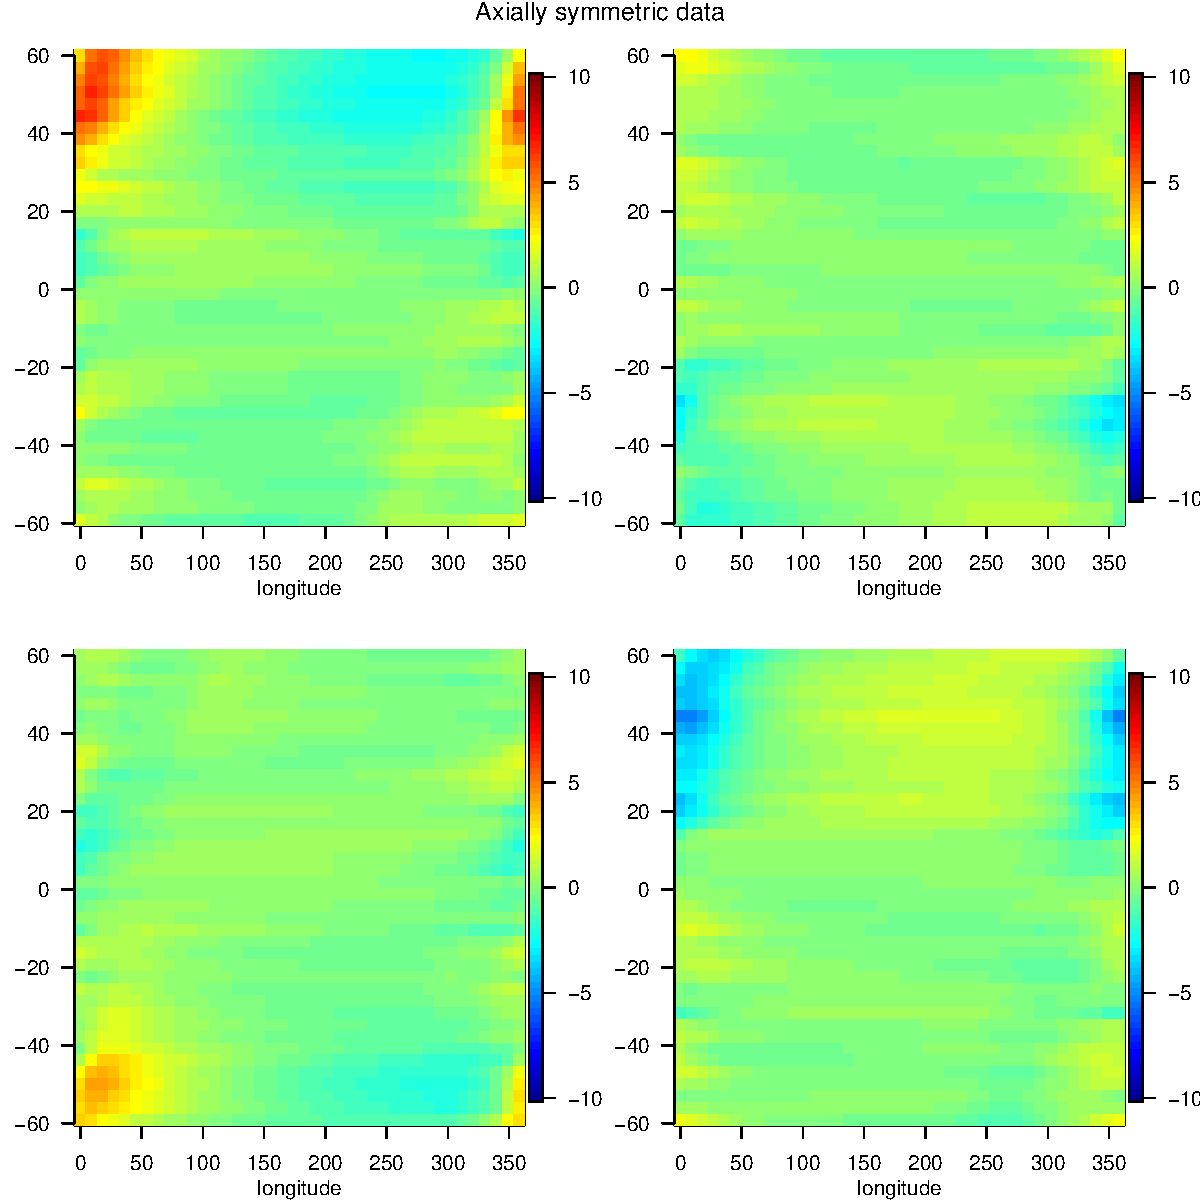
\includegraphics [width=0.9\textwidth ]{graphs/Data_sample_120_model2.pdf}
		\caption{Four consecutive axially symmetric data snapshots based on model 2, grid resolution $2^0\times 1^0$ (data scale -10 and 10).}
	\end{center}
\end{figure}

The above snapshots are some what compliance with geo-spatial data (MSU and TOMS), clearly there is a spatial trend within each latitude but not within longitudes. We observed some inconsistencies (strong spots) closer to the boundary points of longitudes ($\lambda \rightarrow 0,\lambda \rightarrow 2\pi$) and we have ignored the tilt (approximately $23^0$) of Earth axis, both of these are left out as future studies. The figure \ref{grid_plot_model2_sim2} refers to the second snapshot (top right) of the generated data and it is clearly evident that trends are within latitudes.     

\begin{figure}[H]
	\label{grid_plot_model2_sim2}
	\begin{center}
		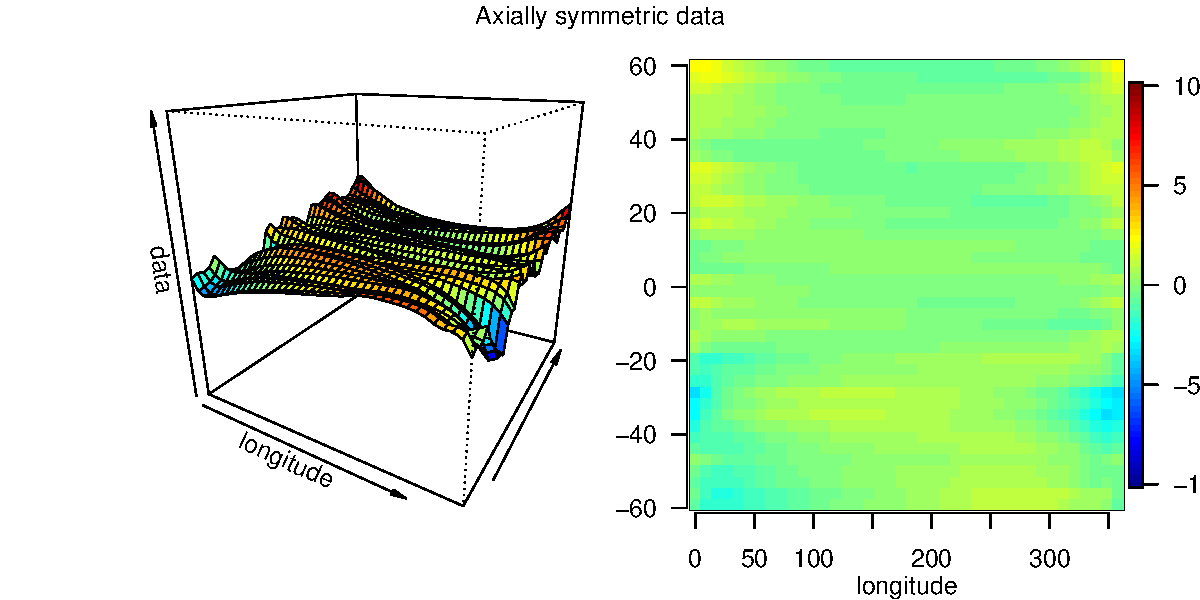
\includegraphics [width=0.9\textwidth ]{graphs/Data_sample_120_model2_density.pdf}
		\caption{One snapshot of the axially symmetric data generated based on model 2, grid resolution $2^0\times 1^0$ (data scale -10 and 10)Data distribution over the grid.}
	\end{center}
\end{figure}

%-------------------------------------% 
\subsection{Comparison of the proposed models with MOM estimates}
%-------------------------------------%

We consider two latitudes with larger latitude difference in order to capture the largest possible errors $70^0S$ and $60^0N$ ($\phi = 10, 150$) with 100 longitudes and compared the MOM estimators.

\begin{figure}[H]
	\begin{subfigure}{.5\textwidth}
		\centering
		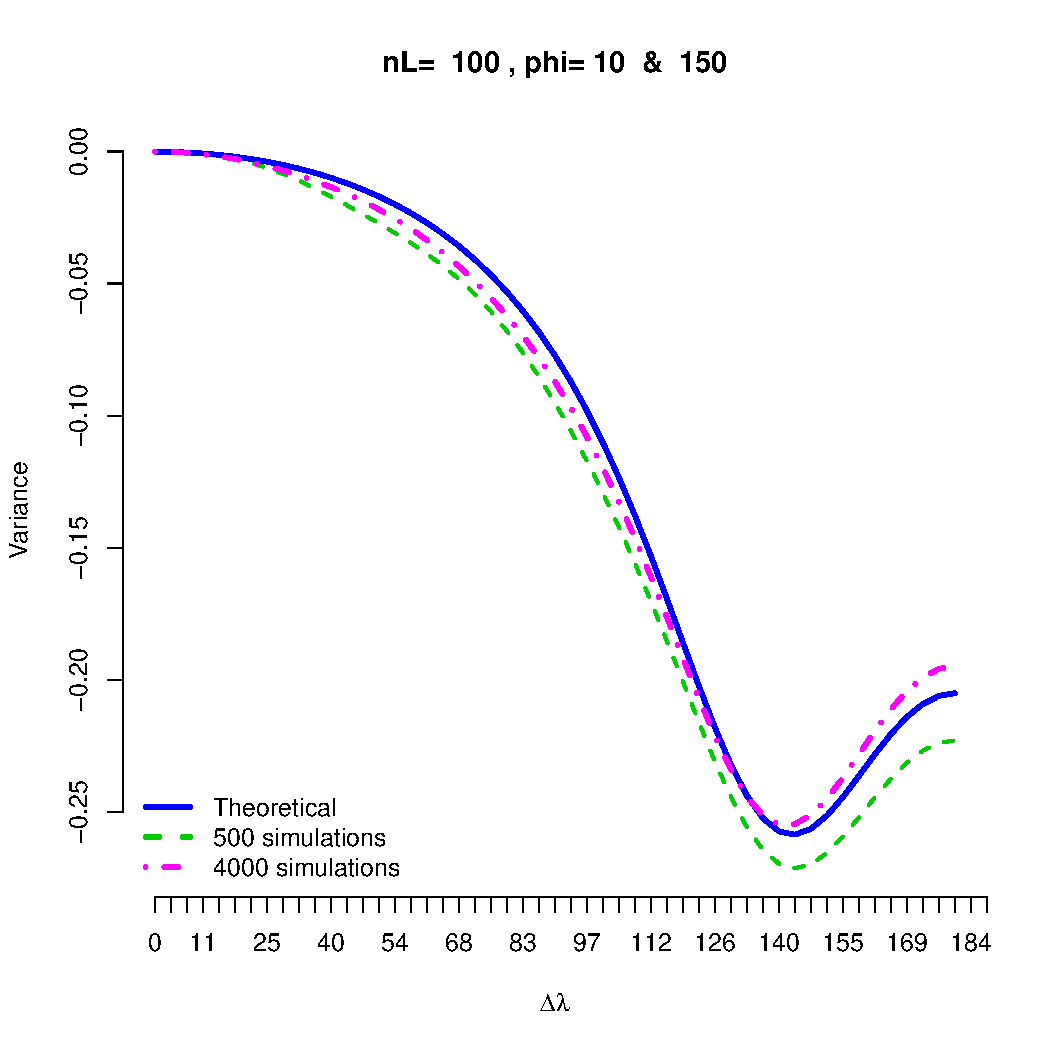
\includegraphics[width=1\linewidth]{graphs/results_variogram_model1}
		\caption{parameter set 1}
		\label{fig:sfig1}
	\end{subfigure}
	\begin{subfigure}{.5\textwidth}
		\centering
		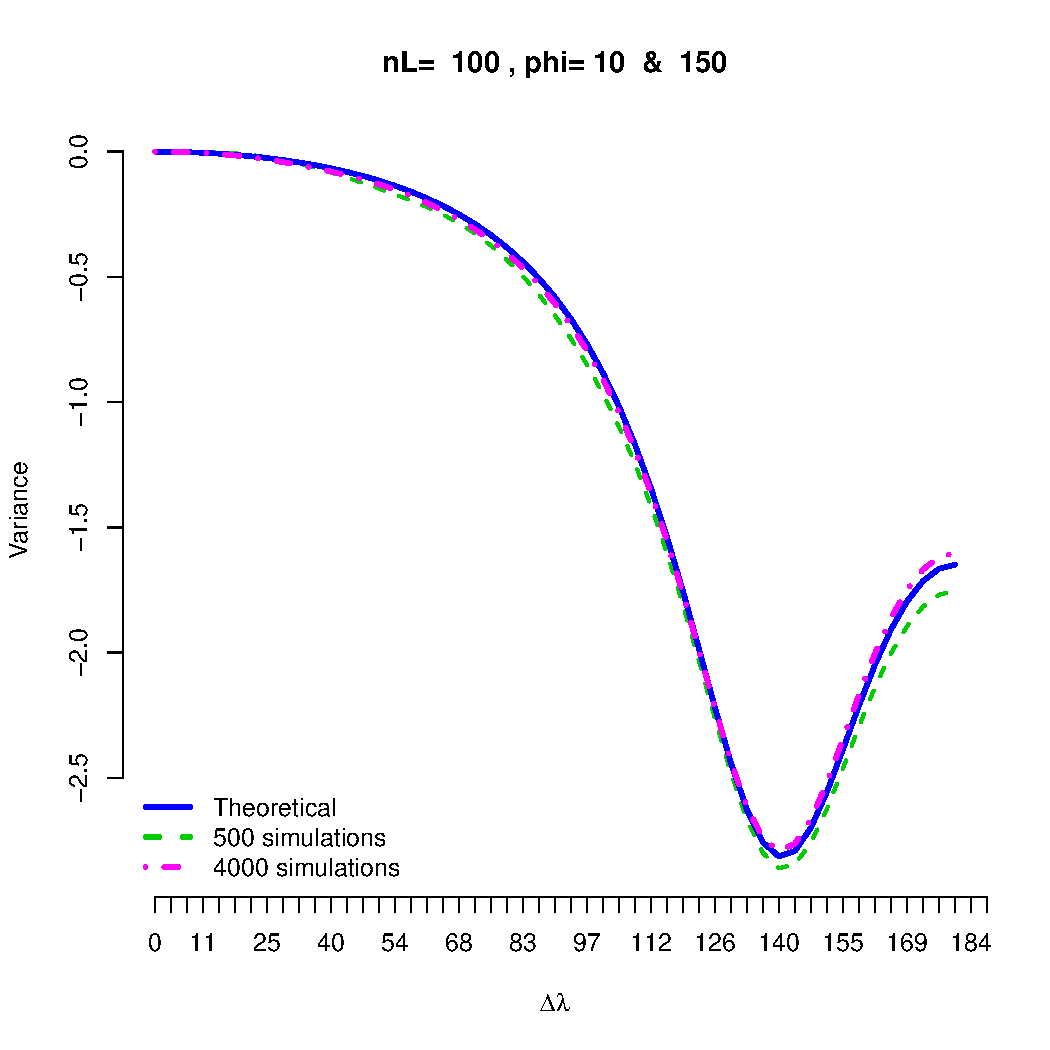
\includegraphics[width=1\linewidth]{graphs/results_variogram_model1_2}
		\caption{parameter set 2}
		\label{fig:sfig2}
	\end{subfigure}
	\caption[Cross variogram estimator comparison]{Cross variogram estimator comparison for covariance model1 }
	\label{compare_varigram_sim}
\end{figure}

The cross variogram estimator (\ref{cross_variogram}) is unbiased and in case of circle we showed that the variogram estimator is inconsistent and we expect a similar result in the case of sphere (the proof is left out as future work). Since model 1 is a non zero mean process we use the cross variogram estimator () to compare the generated data. We used two different sets of parameters to compare the cross variogram for model 1, set 1 $C_1 = 1, C_2 = 1, a = 1, u = 1$ and $p=0.5$ and set 2 $C_1 = C_2 = 2, a = =3, u = 1$ and $p=0.6$. The rate of convergence (\blue{should we talk about any theoretical properties of convergence since we don't have a proof for consistency}) is very slow as one can see that when number of simulations were increased from 500 to 4000 the cross variogram estimator is much closer to its theoretical value. However, the cross variogram estimator for model 2 and 3 converges much faster compared to model 1.  

%-------------------------------------% 
\subsubsection{Results for longitudinally reversible processes}
%-------------------------------------%

The parameter $u = 0$ yields a longitudinally reversible processes on a sphere (see Figure \ref{fig_parameter_comp} 1(d) ) regardless of the model. Now the cross variogram estimator converges ({\em a.s.}) to its theoretical value much faster (< 500 simulations).          

\begin{figure}[H]
	\centering
	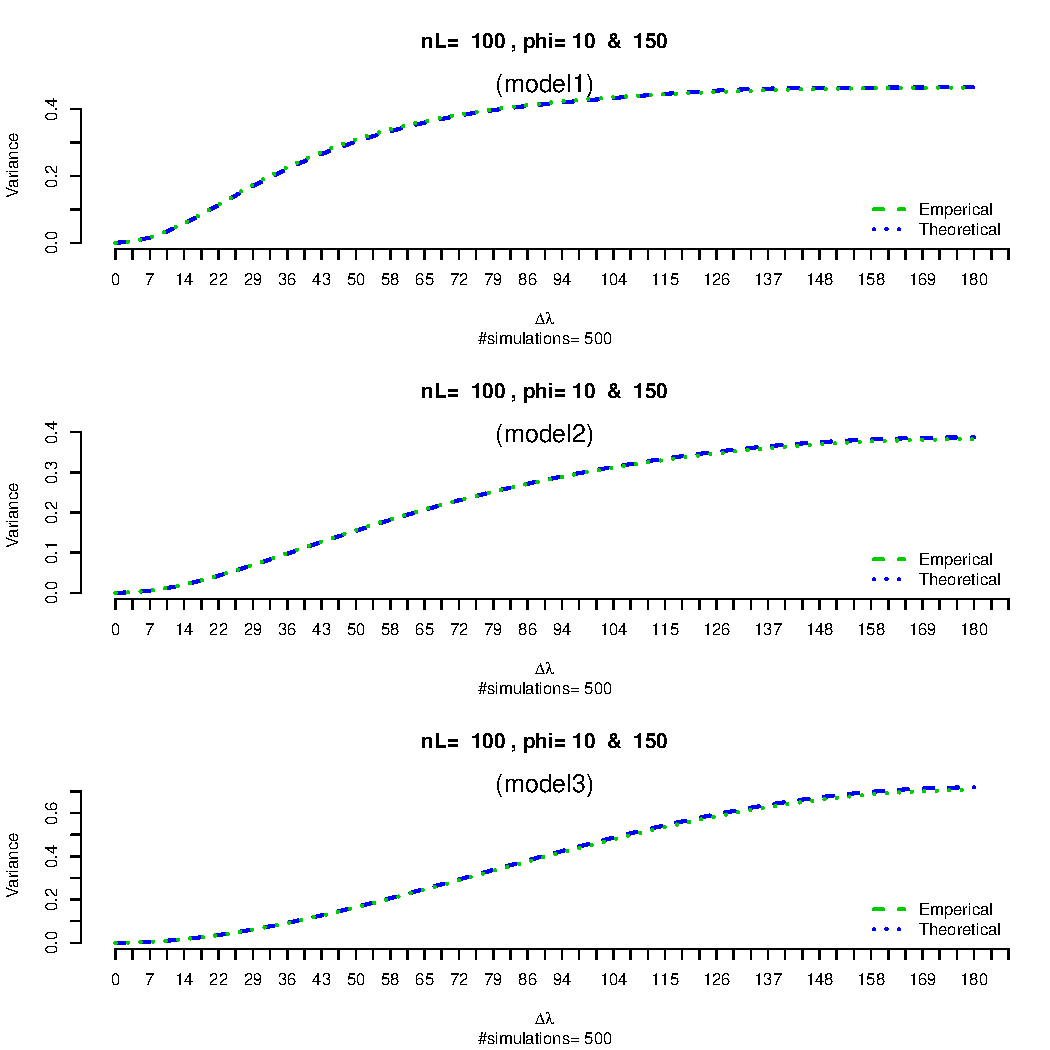
\includegraphics [width=0.9\textwidth ]{graphs/results_variogram_comparison}
	% width=12cm,height=12cm
	\caption[Variogram comparison]{Cross variogram estimator comparison over model 1, model 2, model 3 when $u=0$ }
\end{figure}

Next, we compared the cross covariance estimator on zero mean processes (model 2, model 3) on a sphere. In order to compare the cross covariance we used two pairs of latitudes $20^0S$ with $10^0S$ ($\phi = 70, 80$) and $30^0S$ with $40^0N$ ($\phi = 60, 120$). In a zero mean process, the rate of convergence depends on the distance between the latitudes.    

% \begin{figure}[H]
% \begin{center}
% 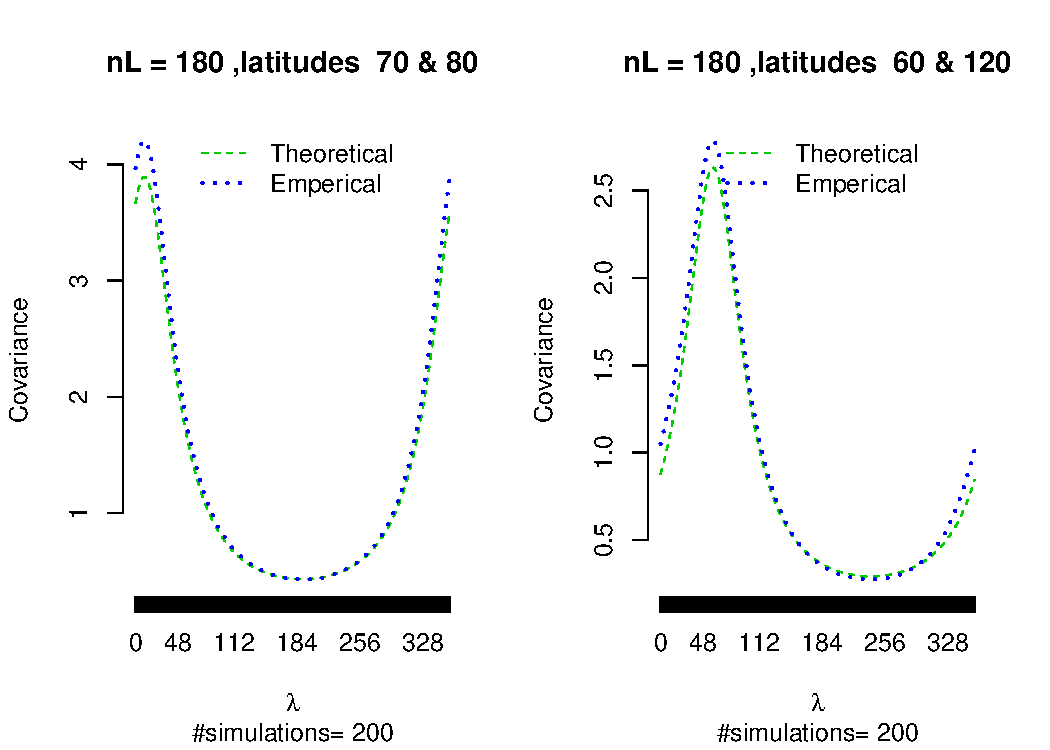
\includegraphics [width=0.75\textwidth ]{graphs/Model1.pdf}
% \caption{Cross covariance comparison of model1}
% \end{center}
% \end{figure}



\begin{figure}[H]
	\begin{center}
		\includegraphics [width=0.75\textwidth ]{graphs/Model2.pdf}
		%\includegraphics [width=6in, height=3in]{Model2.pdf}
		\caption{Cross covariance comparison of model 2}
	\end{center}
\end{figure}


\begin{figure}[H]
	\begin{center}
		%\includegraphics [scale=.6]{Model3.pdf}
		\includegraphics [width=0.75\textwidth ]{graphs/Model3.pdf}
		\caption{Cross covariance comparison of model 3}
	\end{center}
\end{figure}




%\end{document}

	


%%------------------------------------------------------------------%%
\chapter{Future Research (due August 28)}
%\documentclass[12pt, amstex, letterpaper] {report} %{article}


\usepackage[margin=1in]{geometry}
\topmargin -0.5in \textwidth 6.5in \textheight 9in
\footskip .5in
\headheight 0.3in


\usepackage{Sweave}

\DefineVerbatimEnvironment{Sinput}{Verbatim} {xleftmargin=0em,frame=single}
\DefineVerbatimEnvironment{Soutput}{Verbatim} {xleftmargin=0em,frame=single}

\usepackage{amssymb, mathrsfs, amsmath, amsfonts}
\usepackage{enumerate, comment}
\usepackage{hyperref, natbib,apalike, float} %cite
\usepackage{color, multirow, setspace, fancyhdr,graphicx}
\usepackage{undertilde}
\usepackage[bottom]{footmisc}
\usepackage{graphicx}
\usepackage{framed}
\usepackage{subcaption}
\usepackage{amsthm}

%\doublespacing
\pagestyle{empty}
\pagestyle{fancy}
\lhead{ }
%\rhead{May 2016}
\fancyfoot{ }
\rfoot{Dissertation $|$ \thepage}
\lfoot{Chris Vanlangenberg}
\date{}

\includecomment{comment}

\newtheorem{theorem}{Theorem}[section]
\newtheorem{defn}{Definition}[section]
\newtheorem{prop}{Proposition}
\newcommand{\pro}[1]{\begin{prop}{#1}\end{prop}}

%\newtheorem{proof}{proof}
\newtheorem{rmk}{Remark}
\newcommand{\rmark}[1]{\begin{rmk}{#1}\end{rmk}}

\numberwithin{equation}{section}
\renewcommand{\footrulewidth}{0.1pt}
\renewcommand{\headrulewidth}{0.1pt}


\newcommand{\eqn}[1]{\begin{equation}{#1}\end{equation}}

\newcommand{\beq}{\begin{equation}}
\newcommand{\eeq}{\end{equation}}
%\renewcommand\refname{Literature}
\newcommand{\blue}[1]{\textcolor{blue}{\emph{#1}}}
\newcommand{\red}[1]{\textcolor{red}{\emph{#1}}}
\newcommand{\twoc}[2]{{\textcolor{blue}{#1}} and {\textcolor{red}{#2}}}


\newcommand{\xn}{x_1,\ldots, x_n}
\newcommand{\Xn}{X_1,\ldots, X_n}
\newcommand\floor[1]{\lfloor{#1}\rfloor}
\newcommand\ceil[1]{\lceil{#1}\rceil}

\newcommand{\X}{\mathcal{X}}
\newcommand{\Sp}{\mathbb{S}}
\newcommand{\R}{\mathbb{R}}
\newcommand{\C}{\mathbb{C}}
\newcommand{\pd}{positive definite }



\newcommand{\code}[1]{{\small\texttt{#1}}}
\newcommand{\pkg}[1]{{\normalfont\textsf{#1}}}
\newcommand{\var}[1] {{\normalfont\textbf{#1}}}
\newcommand{\Cm}{$C_m(\phi_P, \phi_Q)\ $}

\newcommand{\jun}{\cite{JunStein2008}}
%\begin{document}

In this dissertation research, we focus on data generation and estimation for axially symmetric processes on the sphere. We first show that for the stationary random process on the circle, the commonly used covariance function estimator based on Method of Moments (MOM) is biased with non-estimable bias, while the unbiased MOM variogram estimator is inconsistent. Our second project emphasizes on data generation, in which the axially symmetric random process can be decomposed as Fourier series on circles, where the Fourier random coefficients can be expressed as circularly-symmetric complex random vectors. We develop an algorithm that generates axially symmetric data with the given covariance model. All of the above results and theories have been supplemented via simulations. 

We can extend this dissertation work to a number of future research areas. We will first explore the unbiasedness and consistency of the MOM covariance and variogram estimators for homogeneous and axially symmetric random processes on the sphere. In particular, we expect a similar result holds for axially symmetric random processes. On the other hand, we will also explore the ergodic condition (if exists) that ensures the consistency of these estimators.

We have noticed that our proposed data generation algorithm assumes the closed form of $C_m(\phi_P, \phi_Q)$, which sometimes may not be available. This might restrict the applicability of our data generation algorithm. Note that in order to implement the algorithm, we only need the $C_m(\phi_P, \phi_Q)$ over the gridded locations. Therefore, given the covariance structure $R(P, Q)$, we may use the Discrete Fourier Transform to obtain those gridded $C_m(\phi_P, \phi_Q)$ values. This would definitely complement our dissertation research.

Kriging, or making predictions at unobserved locations, has always been one of the important applications of data modeling and analysis in spatial statistics. With the complexity and dimensionality of global data, it is highly demanded that practically useful parametric models with interpretable parameters would be available for geography and environmental scientists. As the continuation of this dissertation research, we wish to enhance the kriging techniques and make use of proposed global data generation methods to make global predictions with less dimensionality.

%\end{document}

%%------------------------------------------------------------------%%
%%------------------------ Bibliography ----------------------------%%
%%------------------------------------------------------------------%%
%% Replace the myreferences with the name of your bib file.  Then you
%% can run bibtex as usual.  See tips for details.
%%------------------------------------------------------------------%%

\bibliography{biblography}
\bibliographystyle{amsalpha}

%%------------------------------------------------------------------%%
%%------------------------- Appendices -----------------------------%%
%%------------------------------------------------------------------%%
%% If you choose not to have appendices, comment out the \appendix
%% line and the chapters below.
%%------------------------------------------------------------------%%
%\appendix
%\chapter{Appendix Title Goes Here}
%Appendix material goes here.

%%------------------------------------------------------------------%%
\backmatter % required
%%------------------------------------------------------------------%%
%%----------------------- YOU ARE FINISHED ! -----------------------%%
%%------------------------------------------------------------------%%

\end{document}
